\documentclass[12pt,]{report}
\usepackage{lmodern}
\usepackage{amssymb,amsmath}
\usepackage{ifxetex,ifluatex}
\usepackage{fixltx2e} % provides \textsubscript
\ifnum 0\ifxetex 1\fi\ifluatex 1\fi=0 % if pdftex
  \usepackage[T1]{fontenc}
  \usepackage[utf8]{inputenc}
\else % if luatex or xelatex
  \ifxetex
    \usepackage{mathspec}
    \usepackage{xltxtra,xunicode}
  \else
    \usepackage{fontspec}
  \fi
  \defaultfontfeatures{Mapping=tex-text,Scale=MatchLowercase}
  \newcommand{\euro}{€}
    \setmainfont{Times New Roman}
\fi
% use upquote if available, for straight quotes in verbatim environments
\IfFileExists{upquote.sty}{\usepackage{upquote}}{}
% use microtype if available
\IfFileExists{microtype.sty}{%
\usepackage{microtype}
\UseMicrotypeSet[protrusion]{basicmath} % disable protrusion for tt fonts
}{}
\ifxetex
  \usepackage[setpagesize=false, % page size defined by xetex
              unicode=false, % unicode breaks when used with xetex
              xetex]{hyperref}
\else
  \usepackage[unicode=true]{hyperref}
\fi
\hypersetup{breaklinks=true,
            bookmarks=true,
            pdfauthor={},
            pdftitle={},
            colorlinks=true,
            citecolor=blue,
            urlcolor=blue,
            linkcolor=magenta,
            pdfborder={0 0 0}}
\urlstyle{same}  % don't use monospace font for urls
\setlength{\parindent}{0pt}
\setlength{\parskip}{6pt plus 2pt minus 1pt}
\setlength{\emergencystretch}{3em}  % prevent overfull lines
\setcounter{secnumdepth}{0}

\date{}
%set margin specifics
\usepackage[a4paper,left=2.6cm,right=2.4cm,top=2.54cm,bottom=2.54cm]{geometry}
%set unicode
\usepackage[utf8]{inputenc}
\usepackage{fontspec}
%set chinese language support
\usepackage{xeCJK}
%\usepackage[english,russian,greek,ngerman,french]{babel}
%set font
%Chinese bold font specified by other font, using BoldFont=...
\setCJKmainfont[BoldFont=SimHei]{SimSun}
%\setCJKmainfont{FangSong}
%set indent for paragraph
\setlength{\parindent}{2.8em}
%set graphics support
\usepackage{graphicx}
%setting line spaceing
%%\linespread{1.3}
\renewcommand{\baselinestretch}{1.5}
%set fontsize
%\usepackage{anyfontsize}
%\fontsize{15pt}{1.5}

%number equation in section
%\numberwithin{equation}{section}

%use boldface in latex equation
\usepackage{bm}

%change chapter caption to Chinese
\usepackage{titlesec}
\titleformat{\chapter}[display]{\vspace{-4.5ex} \normalfont\centering\huge\bfseries}{第 \thechapter 章}{20pt}{\Huge}
%\titleformat{\chapter}[display]{\normalfont\centering\huge\bfseries}{第 \thechapter 章}{20pt}{\Huge}
%\titleformat{\chapter}[display]
%  {\normalfont\huge\bfseries}{\filcenter\underline{\MakeUppercase{\textls[400]{\chaptertitlename}}\
%  \thechapter}}{20pt}{\Huge}

% use the script English letter 
%\mathcal{Z} 
\usepackage{amssymb}
%\usepackage{mathrsfs}
%\mathscr{L}

\renewcommand{\contentsname}{目录}
\renewcommand{\figurename}{图}

%biblatex bibliography indent
\usepackage{biblatex}
\setlength{\bibhang}{11pt}

% header and footer
\usepackage{fancyhdr}
\pagestyle{fancy}
%\fancyhead[LE,RO]{\leftmark}
%\fancyhead[RE,LO]{硕士毕业论文}
%\lhead{}
%\chead{第\thechapter 章 }
%\rhead{}
%\renewcommand{\chaptermark}[1]{\markboth{第\thechapter 章\ #1}{}}

% toc header and footer setting
\usepackage{tocloft}
\tocloftpagestyle{plain}

%add content line to "toc" as a "chapter" entry with name "reference"
%\addcontentsline{toc}{chapter}{reference}

\begin{document}

\pagenumbering{Roman} \vspace*{0.0cm}

\begin{center}
\Large \textbf{光激发下共轭聚合物中激子形成与载流子输运的动力学机制的研究}
\end{center}\vspace{0.54cm}\begin{center}
\Large \textbf{摘要}
\end{center}

\pagestyle{plain}
%\pagestyle{fancy}

\vspace{1.5cm}

\addcontentsline{toc}{chapter}{摘要}

共轭聚合物在半导体行业中有着诸多应用:聚合物发光二极管,聚合物场效应管和
聚合物太阳能电池。聚合物太阳能的研究随着人们对环境保护以及新能源意识的加强而得
到了诸多的关注。本文的讨论也针对Alan
Heeger对聚合物太阳能电池研究中的两个结果展开:
(1)激子的形成过程;(2)带电载流子的输运。

运用分子动力学方法可以用来揭示激子形成的过程,其可以被分解为两个部分 :
电子空穴对的局域和弛豫。在光激发的作用下,电子的跃迁促使电子空穴对迅速形成与局域,
并引起了聚合物体系的能量发生剧烈的变化。40飞秒后,在这种变化下使得光激发过程进入第二个
阶段:弛豫。体系的总能量,晶格的能量和电子的能量在弛豫过程进行到850飞秒的时候达到稳定
值,此时的晶格位型和电子空穴对依然保持局域状态,这个能量保持稳定的局域状态称为激子态
。因为电子空穴的局域早于激子的形成,所以在聚合物太阳能电池中电子空穴对极有可能在激子
形成之前就发生了分离。全文以第一作者发表于 \emph{Journal of Physical
Chemistry B}。

在体异质结聚合物太阳能电池,激子在异质结中分离后,一个带有负电荷的极化子沿着聚
合物链输运到受体处,这个过程对在聚合物太阳能电池中载流子的输运性质有重要影响。在负极
化子输运的过程中,由于外界光激发的作用,极化子会被激发而形成局域,并伴随键长的改变。
激发后的极化子的输运速度对比处于基态的极化子而言变慢了。此外,极化子在聚合物链
上输运的速率极大的受到光激发作用的影响,光强的增大会导致被激发的极化子的局域化更深
,从而降低了极化子输运的速率。总之,聚合物太阳能电池中深度自陷的载流子给了纳米尺度下
的储存和成像设备提供了启示。全文以第一作者发表于 \emph{Nanoscale}。

\vspace{1.5cm}

\noindent
\large 
\textbf{关键词: 激子,局域,半导体聚合物,太阳能电池,极化子,输运,光激发}

\clearpage

\vspace*{0.0cm}

\begin{center}
\Large \textbf{DYNAMICS OF EXCITON FORMATION AND CHARGE CARRIER TRANSPORT IN CONJUGATED POLYMER UNDER PHOTOEXCITATION}
\end{center}\vspace{0.54cm}\begin{center}
\Large \textbf{Abstract}
\end{center}

\pagestyle{plain}

\vspace{1.5cm}

\addcontentsline{toc}{chapter}{Abstract}

Conjugated polymer has many applications in the semiconductor industry:
Polymer Light-Emitting Diodes, Polymer Field-Effect Transistor and
Polymer Solar Cell. There are tremendous attention paid to the research
on polymer solar cell as people are getting more aware of environment
protection as well as the comprehension of developing new kind of
energy. This thesis focues on two highly discussed aspects based on the
research of Alan Heeger's group: (1) Charge generation, or excition
formation process; (2) Charge transport, or dynamics of charge carrier
motion in conjuatged polymer system.

Molecule dynamics is empolyed to uncover the time profile of exciton
formation, which can be divided into two stages: the localization of
electron-hole pairs and the relaxation process. Under photoexcitation,
the electron transition rapidly forms the electron-hole pair which also
leads to its localization, which triggers the total energy to shift
violently and oscillate. The oscillation during the first 40 fs induces
the excitation to step into the second stage, i.e., relaxation. After
the relaxation process of about 850 fs, the total energy , lattice
energy and electron energy reach certain values while the lattice
configuration and electron eremain localized, and indicating the
formation of a singlet exciton. Because electron-hole pair is localized
before exciton is formed, it is highly likely that the electron-hole
pair will be separated before the formation of exciton in the process of
conducting polymeric solar cell. The corresponding result has been
published on \emph{Journal of Physical Chemistry B}.

In a real bulk heterojunction polymer solar cell, after exciton
separation in the heterojunction,the resulting negatively-charged
carrier, a polaron, moves along the chain of the acceptor, which is
believed to be of significance for the charged carrier transport
properties in a polymer solar cell. During the negative polaron
transport, due to the external light field, the polaron is re-excited
and induces deep localization, also forming a new local distortion of
the alternating bonds. It is revealed that the excited polaron moves
more slowly than the ground-state polaron. Furthermore, the velocity of
the polaron moving along the polymer chain is crucially dependent on the
photoexcitation. With an increase in the instensity of the optical
filed, the localization of the excited polaron has been deepning, with a
slowing down of the polaron's velocity. Mostly, the deep trapping effect
of charged carrier in composite conjugated polymer solar cell presents
an opportunity for the future application in nanoscale memory and
imaging devices. The corresponding result has been published on
\emph{Nanoscale}.

\vspace{1.5cm}

\noindent
\large 
\textbf{KEY WORDS: localization, exciton, semiconducting polymer, solar cell,
polaron, transport, photoexcitation.
}

\clearpage
 \cleardoublepage
\pagenumbering{gobble} \tableofcontents
\cleardoublepage
\pagenumbering{arabic}

\pagestyle{fancy}

\chapter{半导体聚合物太阳能电池材料介绍}\label{ux534aux5bfcux4f53ux805aux5408ux7269ux592aux9633ux80fdux7535ux6c60ux6750ux6599ux4ecbux7ecd}

\lhead{} \chead{第一章\quad 半导体聚合物太阳能电池材料介绍} \rhead{}

\section{1.1
半导体聚合物的研究进展}\label{ux534aux5bfcux4f53ux805aux5408ux7269ux7684ux7814ux7a76ux8fdbux5c55}

半导体聚合物在通过掺杂等手段处理后,会使其导电性能介于半导体与导体之间。它既有传统
的聚合物所具备的柔韧性、机械性和功能结构易于控制等特性,同时拥有不逊于金属的导电性。\textsuperscript{{[}1{]}}半导体聚合物可以分为两大类,共轭聚合物与复合型聚合物。如果聚合物本身拥有或经过
掺杂处理后具有导电性,这类聚合物称为共轭聚合物;如果聚合物本身无法通过简单的掺杂等
手段使其具有导电性,这类聚合物称为复合型聚合物。复合型聚合物在一定方式下通过加入导
电材料复合而成。\textsuperscript{{[}2{]},{[}3{]},{[}4{]}}

半导体聚合物链一般由单双键交替组成了一种共轭体系,这种共轭体系称为\(\pi\)体系。这种
体系下的电子可以在聚合物链上运动而使得该聚合物具备了导电性。虽然\(\pi\)电子的存在为聚
合物的导电性提供了基础,但正如前文提到过的一样,并非所有聚合物都拥有易导电的特性。
这还需要从能带结构来给予解释:如果在聚合物链中,派尔斯不稳定性会使得导带与价带之间
的能隙比较大,导致\(\pi\)电子通过简单的激发并达到导带的几率非常低。因此,在室温常压等
条件下,导带中的电子占据就会很少,所以电导率会变得非常低,没有表现出可观的导电性。
如果通过氧化反应使得聚合物链失去电子(或者通过还原反应使得聚合物链得到电子),聚合
物链的能隙中间就会出现新的载流子:激子,极化子或者双极化子;从而使得聚合物链产生导
电性。\textsuperscript{{[}5{]},{[}6{]}}
除了对聚合物进行氧化还原反应激发新的载流子使其导电以外,Heeger,
MacDiarmid和Shirakawa等在1977年发现,聚乙炔中掺杂碘后其导电性提高了几个
甚至几十个数量级。这一发现不仅让这三位科学奖共同获得了2000年诺贝尔化学奖
,\textsuperscript{{[}7{]},{[}8{]},{[}9{]}}而且使得半导体聚合物得到了空前的关注,并逐渐使
其发展为一个新型的交叉学科领域。
在随后的研究中发现,除了聚乙炔具备掺杂后的强导电性,还有非常多的具有共轭\(\pi\)体系的
有机聚合物在掺杂后获得了良好的导电性,例如聚对苯,聚对苯撑乙烯,聚噻吩等。

半导体聚合物优良的导电性以及特殊的光学特性使其本身在自然科学领域中成为理想的应用材
料。半导体聚合物的常见应用有: 聚合物发光二极管 (Polymer Light-Emitting
Diodes), 聚合物场效应管 (Polymer Field-Effect Transistor),
和聚合物太阳能电池 (Polymer Solar Cell)。

聚合物发光二极管的研究可以追溯到20世纪50年代。Bernanose以及其合作
者通过对吖啶橙类物质加电压后发现了电致发光现象。\textsuperscript{{[}10{]},{[}11{]},{[}12{]},{[}13{]}}
1960到1963年,Pope 等人发现了空穴被注入到了有机晶体蒽 (Anthracene
Crystal)
的现象,并对电子与空穴的注入接触做了解释。\textsuperscript{{[}14{]},{[}15{]},{[}16{]}}在此期间
,他们还首次从有机
晶体蒽中观察到了通电引起的发光现象。\textsuperscript{{[}17{]}} 1965年,
加拿 大科学家 Helfrich 和 Schneider
第一次实现了有机单晶蒽中的双注入重合的电致发光。\textsuperscript{{[}18{]}}
最早的聚合物薄膜电致 发光器件是由英国科学家 Partridge
在1975年制成的,其结果发表于1983年。\textsuperscript{{[}19{]},{[}20{]},{[}21{]},{[}22{]}}
就在不久后的1987年,Eastman Kodak 公司的 Tang 与 Slyke 共同制备
了首个聚合物发光二极管。\textsuperscript{{[}23{]}}
这标志了现代聚合物发光二极管研究领域的 开始。在随后的
1990年,剑桥大学卡文迪许实验室 (Cavendish Laboratory) 的 Burroughes
等人报道了 首个较高效率的有机发光二极管,
他们的材料是基于聚对亚苯基亚乙烯基 -- poly(p-phenylene
vinylene)。\textsuperscript{{[}24{]}} 他们制备的器件在直流驱 动偏压小于
14V 的时候有蓝绿色光输出,其量子效率达到了0.05\%。
为了提高有机物发光的量子效率,1988年 Baldo等人让单重态激子 (singlet
exciton) 激子与三重态激子 (triplet exciton) 同时参与
能量的传递,从而使得其内部能量的传输效率提高到90\%。\textsuperscript{{[}25{]}}
1999年, Cao 等人通过在
共轭聚合物中掺杂改善电子传输材料的基团,使得量子效率增加到50\%。\textsuperscript{{[}26{]}}

\begin{figure}[h!]
    \centering
    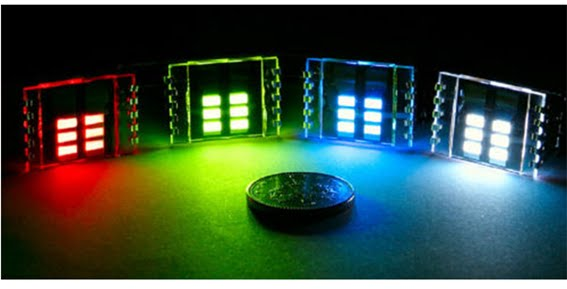
\includegraphics[scale=0.6]{./figures/pled.jpeg}
    \caption{半导体聚合物发光二极管}
    \label{fig:pled}
\end{figure}

半导体聚合物场效应管的研究起源于1954年。研究者在
芳香族碳水化合物薄膜中掺入氯后,发现该薄膜具有导电性,其电导率大致为 0.1
S/cm。\textsuperscript{{[}27{]}}
1986年,Tsumura等人用聚噻吩为材料研制出了世界上第一个有机场效应管。\textsuperscript{{[}28{]}}
因为有机聚合
物场效应管的载流子迁移率低的原因,人们把有机场效应管的研究方向转移到了有机小分子上面
。其中, Garnier 用 \(\alpha-6T\)
为工作原料制备出的场效应管,其载流子迁移率比之前高出了10\textsuperscript{3}个数量级。\textsuperscript{{[}29{]}}
有机小分子高性
能场效应管与无极材料硅为基础的场效应管在载流子迁移率已以及开关电流方面非常接近。但有
机场效应管的制作成本更低,制作工艺简单,使得其应用前进非常被看好。

\begin{figure}[h!]
    \centering
    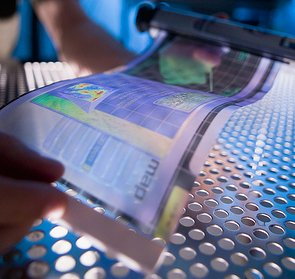
\includegraphics[scale=0.6]{./figures/ofet.jpg}
    \caption{半导体聚合物场效应管为基础的发光设备}
    \label{fig:ofet}
\end{figure}

聚合物太阳能电池的研究也可以追溯到上世纪50年代,已经有巨大的努力投入到了制备更高效的
有机太阳能电池的研究中去。
Kearns等利用有机小分子材料镁酞菁制成最早的有机太阳能电
池。\textsuperscript{{[}30{]},{[}31{]}} 到了上世纪 70
年代,随着多种共轭聚合物薄膜材料的成功合成,如聚乙炔薄膜,
为制备高分子太阳能电池的提供了新型候选材料
,\textsuperscript{{[}32{]},{[}33{]},{[}34{]}}
从而制成了最早的共轭聚合物光电转换材料的聚乙炔薄膜太阳能电池
。\textsuperscript{{[}35{]}}早期有机太阳能电
池被设计成三明治结构,即两个金属电极中间夹着一层有机活性层
。\textsuperscript{{[}36{]}}通过不同功函数的两个
金属电极形成的内电场,拆分光致激子。然而,仅仅依靠利用上述的器件中两个电极上不同功函
数形成的内电场拆分激子极为不易
。\textsuperscript{{[}37{]},{[}38{]},{[}39{]},{[}40{]}}
为了克服上述困难,Tang 等在
1986年率先使用共轭聚合物材料PV和铜酞菁制成聚合物异质结,通过异质结拆分光致激子,将光
电转换效率提高到1\%左右。\textsuperscript{{[}41{]}}这类材料也被称为共轭聚合物异质结光电转
换材料。1992年, Sariciftci
等人在共轭聚合物与富勒烯的连接处观察到了一种极度高效的电荷超快转移现象。\textsuperscript{{[}42{]}}
在这一现象的启发下,人们研制出了聚合物与富勒烯为材料的双层体异质结太阳能电池。\textsuperscript{{[}43{]},{[}44{]},{[}45{]},{[}46{]}}

\begin{figure}[h!]
    \centering
    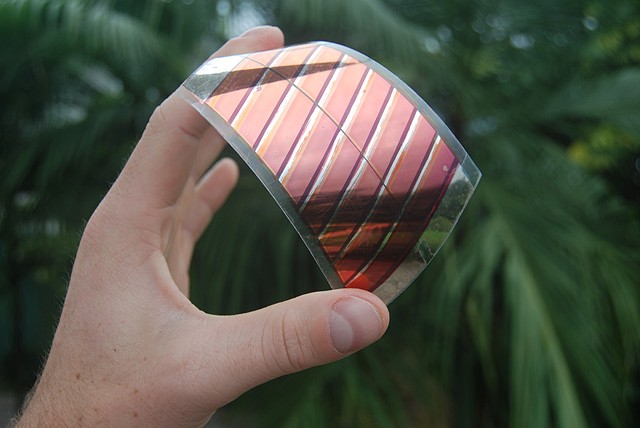
\includegraphics[scale=0.5]{./figures/solarcell.jpg}
    \caption{半导体聚合物太阳能电池}
    \label{fig:solarcell}
\end{figure}

可以看到,有机材料为基础的各种设备在业界的应用会越来越广。而半导体聚合物材料的研究
更是其中最为重要的课题之一。本文将主要关注点放在了共轭聚合物材料导电性质的探究上,对
有机太阳能电池中\textbf{激子的形成过程},\textbf{弛豫过程},以及以极化子为代表的\textbf{载流子输运过
程}进行细致的计算,分析,对有机聚合物太阳能电池的研究中出现的一些问题做出的解释。

\section{1.2
体异质结有机太阳能电池的工作原理}\label{ux4f53ux5f02ux8d28ux7ed3ux6709ux673aux592aux9633ux80fdux7535ux6c60ux7684ux5de5ux4f5cux539fux7406}

有机太阳能电池究竟是如何将光能转化成了电能? 这个过程通常分为四个步骤:
\textbf{(1)}在外界光场的作用下,处于基态的电子吸收光子的能量而被激发到能
带中的导带 ,
同时在价带中会留出一个空位,这个空位成为空穴,空穴带有正电荷。正是由于
光场与库仑相互作用,使得电子空穴对可以一直保持存在并有可能因为弛豫现象而
形成一个能量稳定的电子空穴对状态,这个状态称为激子态。\textsuperscript{{[}47{]}}
\textbf{(2)}
聚合物链中的激子会扩散到电子给体与电子受体的接触层。\textbf{(3)}
在接触层,激子会被解离成为独立的电子与空穴。电子进入受体,空穴保留在给体。电子在聚
合物中会形成一种称为极化子的准粒子。极化子受到外电场的作用下发生运动,形成载流
子。\textbf{(4)}
载流子在经过输运后会到达电极而为电池完成一个充电的过程。此过程中,载流子
本身是一个带有负电荷的极化子,称之为负极化子。
因此,半导体聚合物太阳能电池的与
原理可以概括为四个步骤:激子的形成,激子的扩散,激子的分离,和载流子的输运。

\begin{figure}[h!]
    \centering
    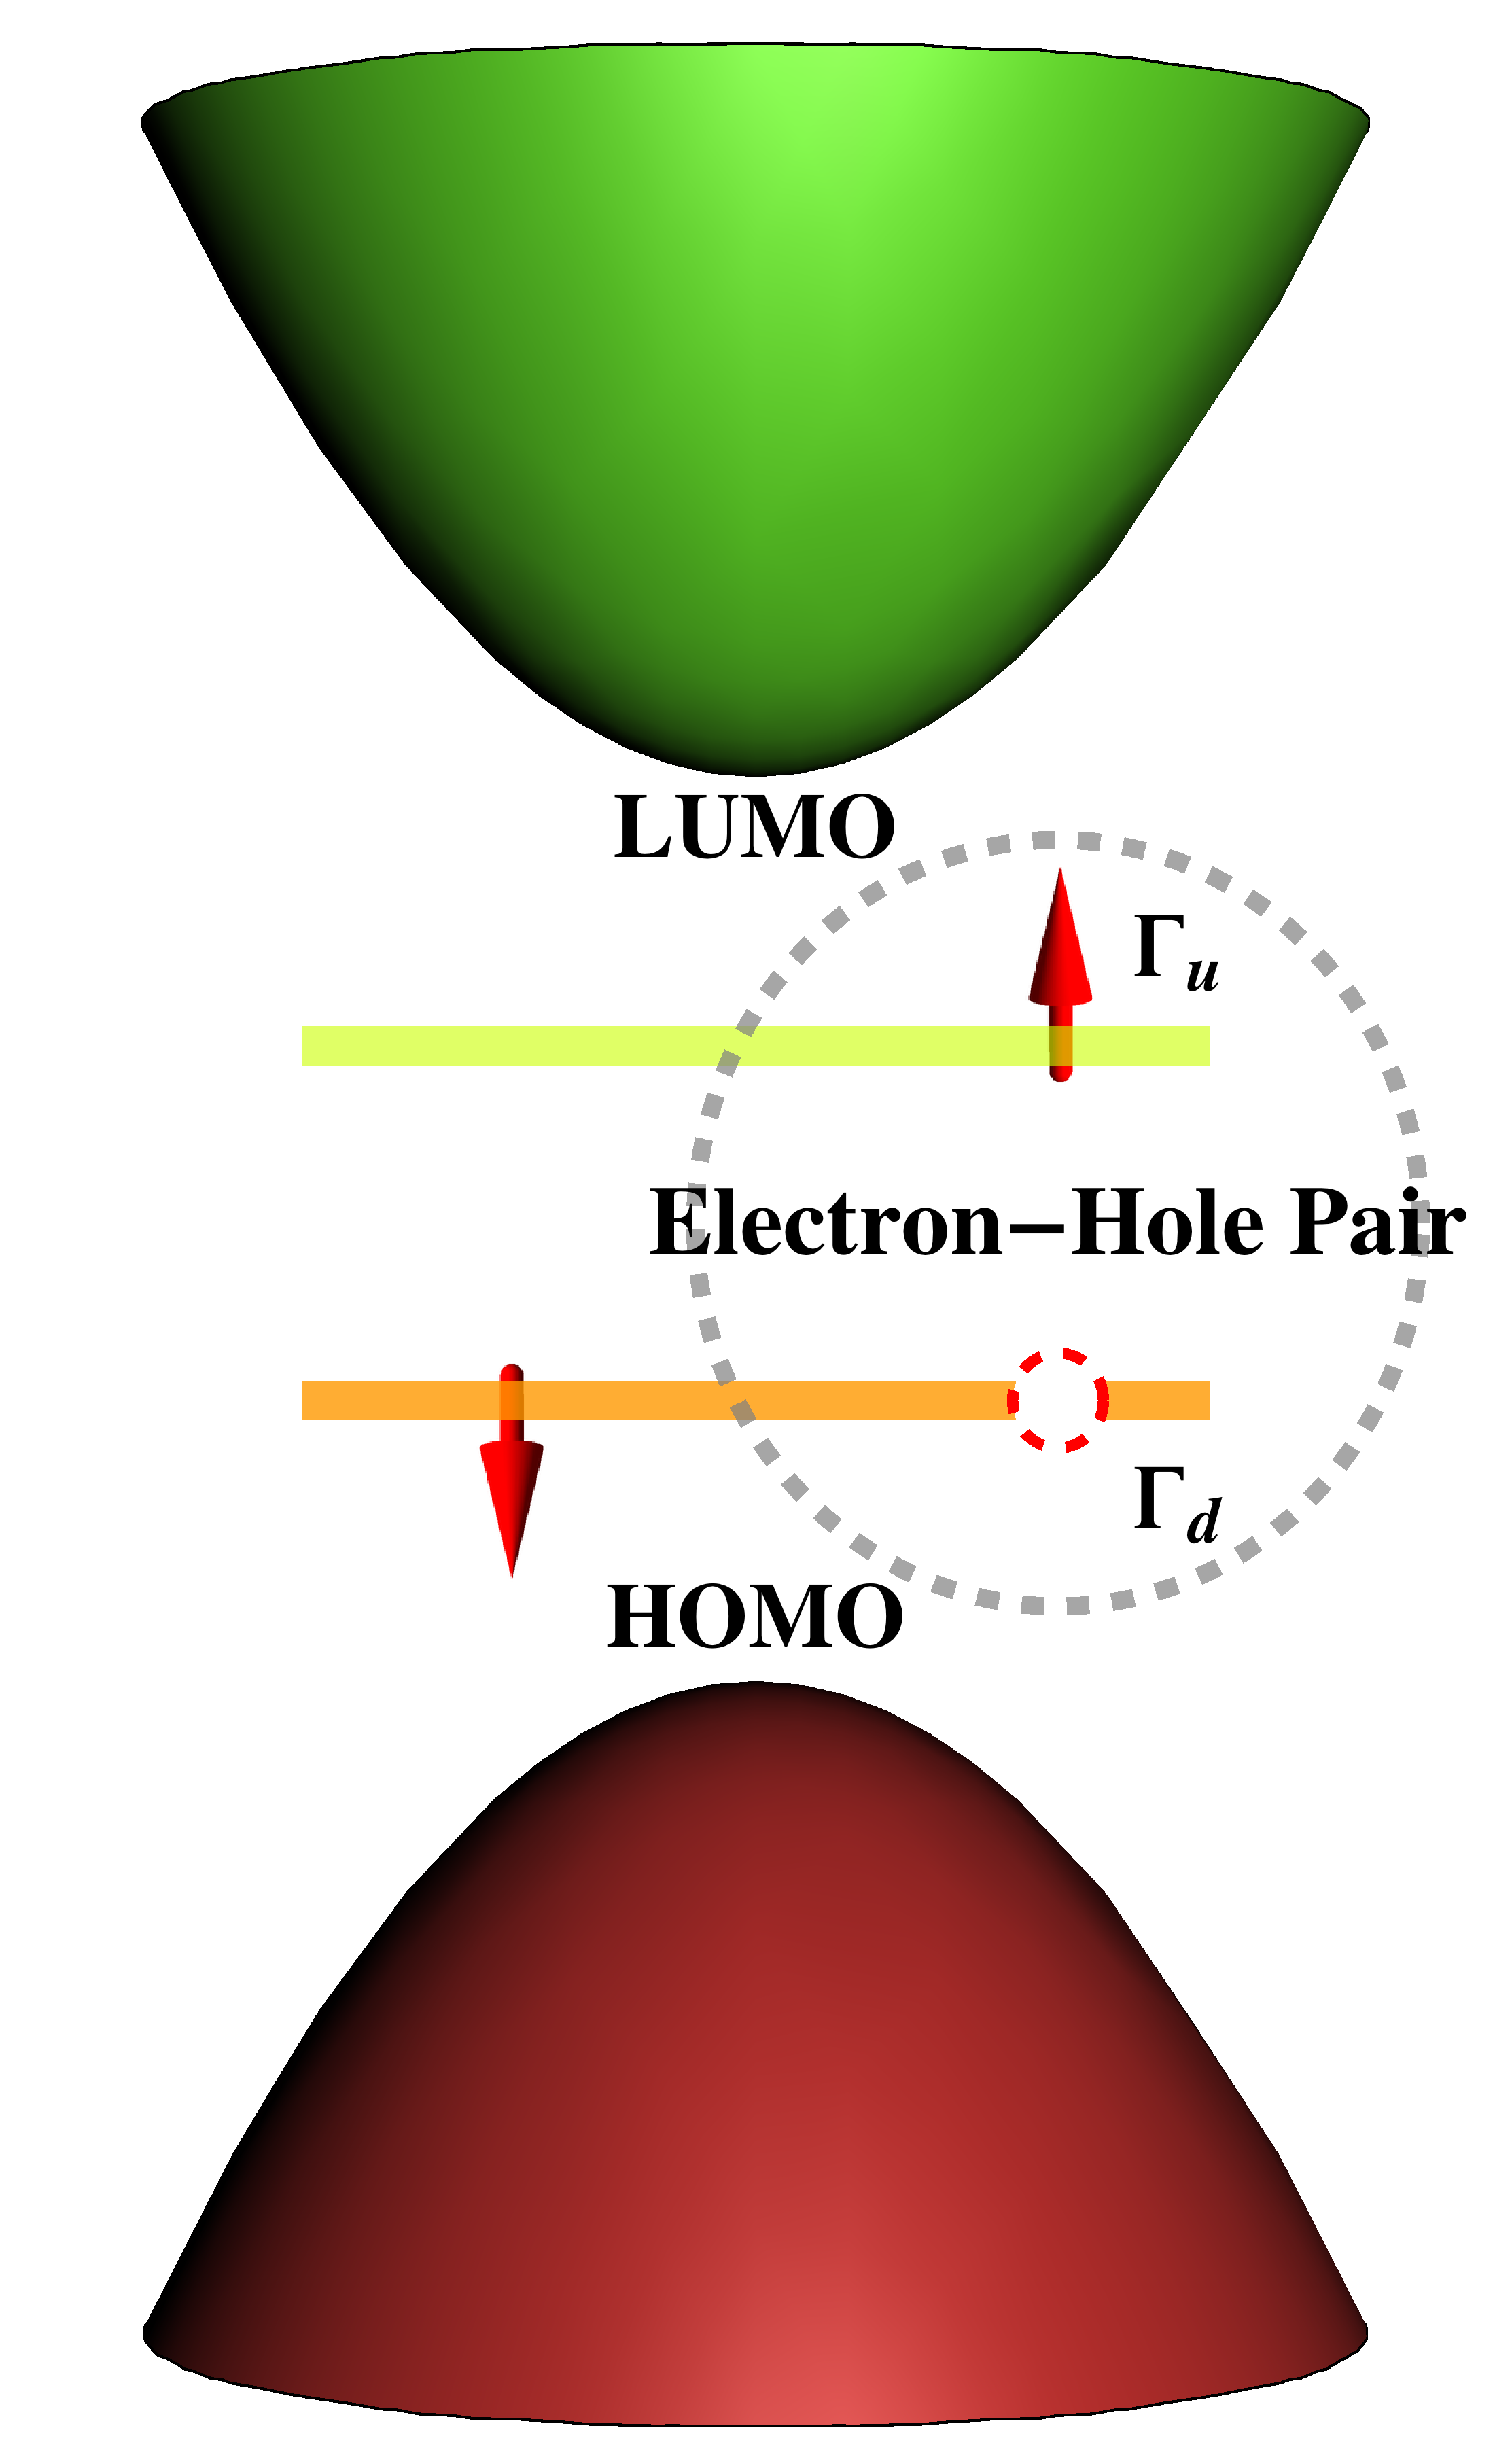
\includegraphics[scale=0.6]{./figures/exciton.png}
    \caption{在能带结构中,光激发下电子受激跃迁形成的激子态}
\end{figure}

\begin{figure}[h!]
    \centering
    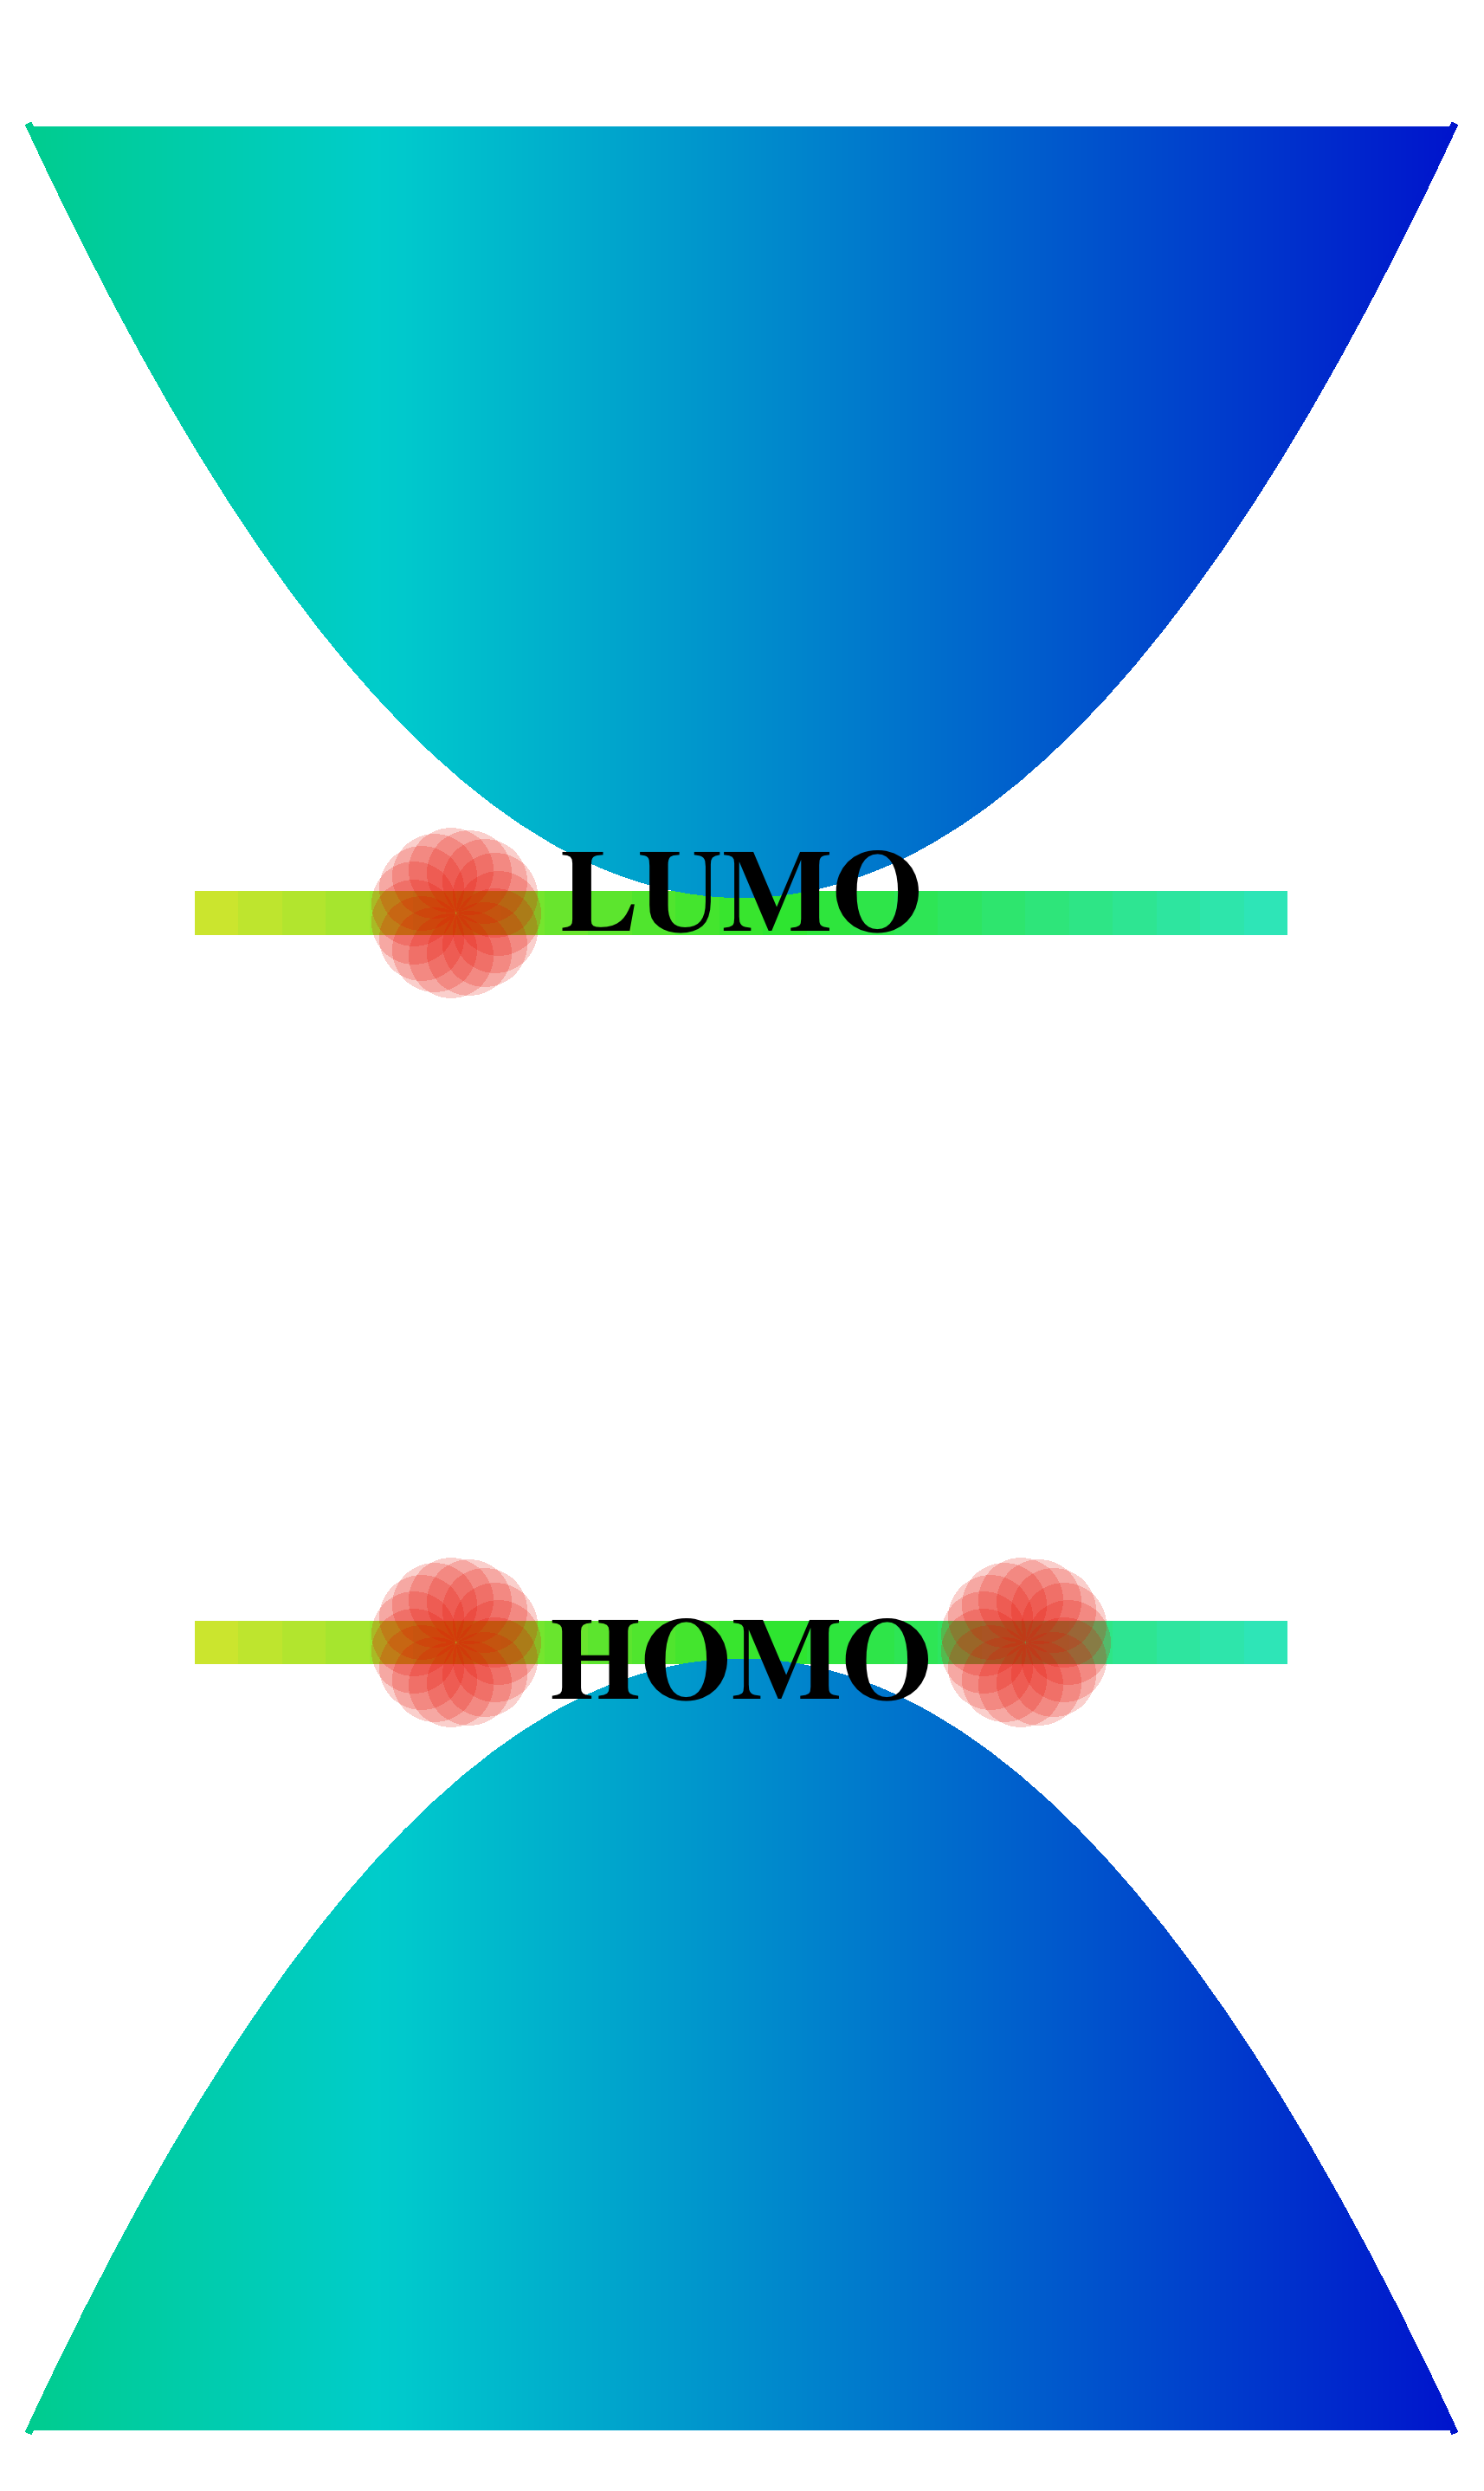
\includegraphics[scale=0.09]{./figures/polaron0.png}
    \caption{在能带结构中,电子注入聚合物引起的能带变化并形成的负极化子}
    \label{fig:npolaron}
\end{figure}

为了得到更高效率的有机太阳能电池,以上的四个步骤中的每一个都值得去研究。在自发辐射
以及非辐射跃迁的条件下,激子会衰变。因此,为了减弱激子的衰变,现在科学家们采用了
缩短子扩散距离的方法。体异质结太阳能电池的结构是有效缩短
激子扩散距离的方法。如图(\ref{fig:solar})所示的是理想情况下的有机体异质结太阳能电池的结构。\textsuperscript{{[}48{]},{[}49{]}}
可见,给体与受体之间有非常理想的充分融合,但是这种理想的体异质结结构在纳米尺度下却很难
制成。因此,工艺上一般将近一维形态的聚合物受体材料溶解在给体材料中,现实工艺中
的体异质结太阳能电池的结构如图(\ref{fig:solar3d})。正是由于这种结构,体异质结随
机的填充了太阳能电池的整个空间,这样的形态使得被外界光激发的激
子容易在全空间与受体与给体的异质结相接触,激子分离前的扩散距离非常短,
降低了激子在扩 散中途湮灭的可能性。实验中,在P3HT (RR-P3HT) 与 PCBM
相分离混合薄膜中可以发现
,大部分激子如前文所述一般被分解成为自由运动的极化子。\textsuperscript{{[}50{]}}在混合薄膜的界面处除了产生带有电荷的极化子
,超快光谱测量还发现一种极化子对的产生。\textsuperscript{{[}51{]}}
导致对于共轭聚合物中的载流子而言,似乎存在着一种带有双倍电荷的载流子,例如双极化子。
在2011年,通过拉曼光谱,人们在寡聚噻吩二价阳离子中观察到了双极化子转换成为极化子对的
现象。\textsuperscript{{[}52{]}}
因此,在激子分离后产生的准粒子中,扮演着载流子角色 的实际上是极化子。

\begin{figure}[h!]
    \centering
    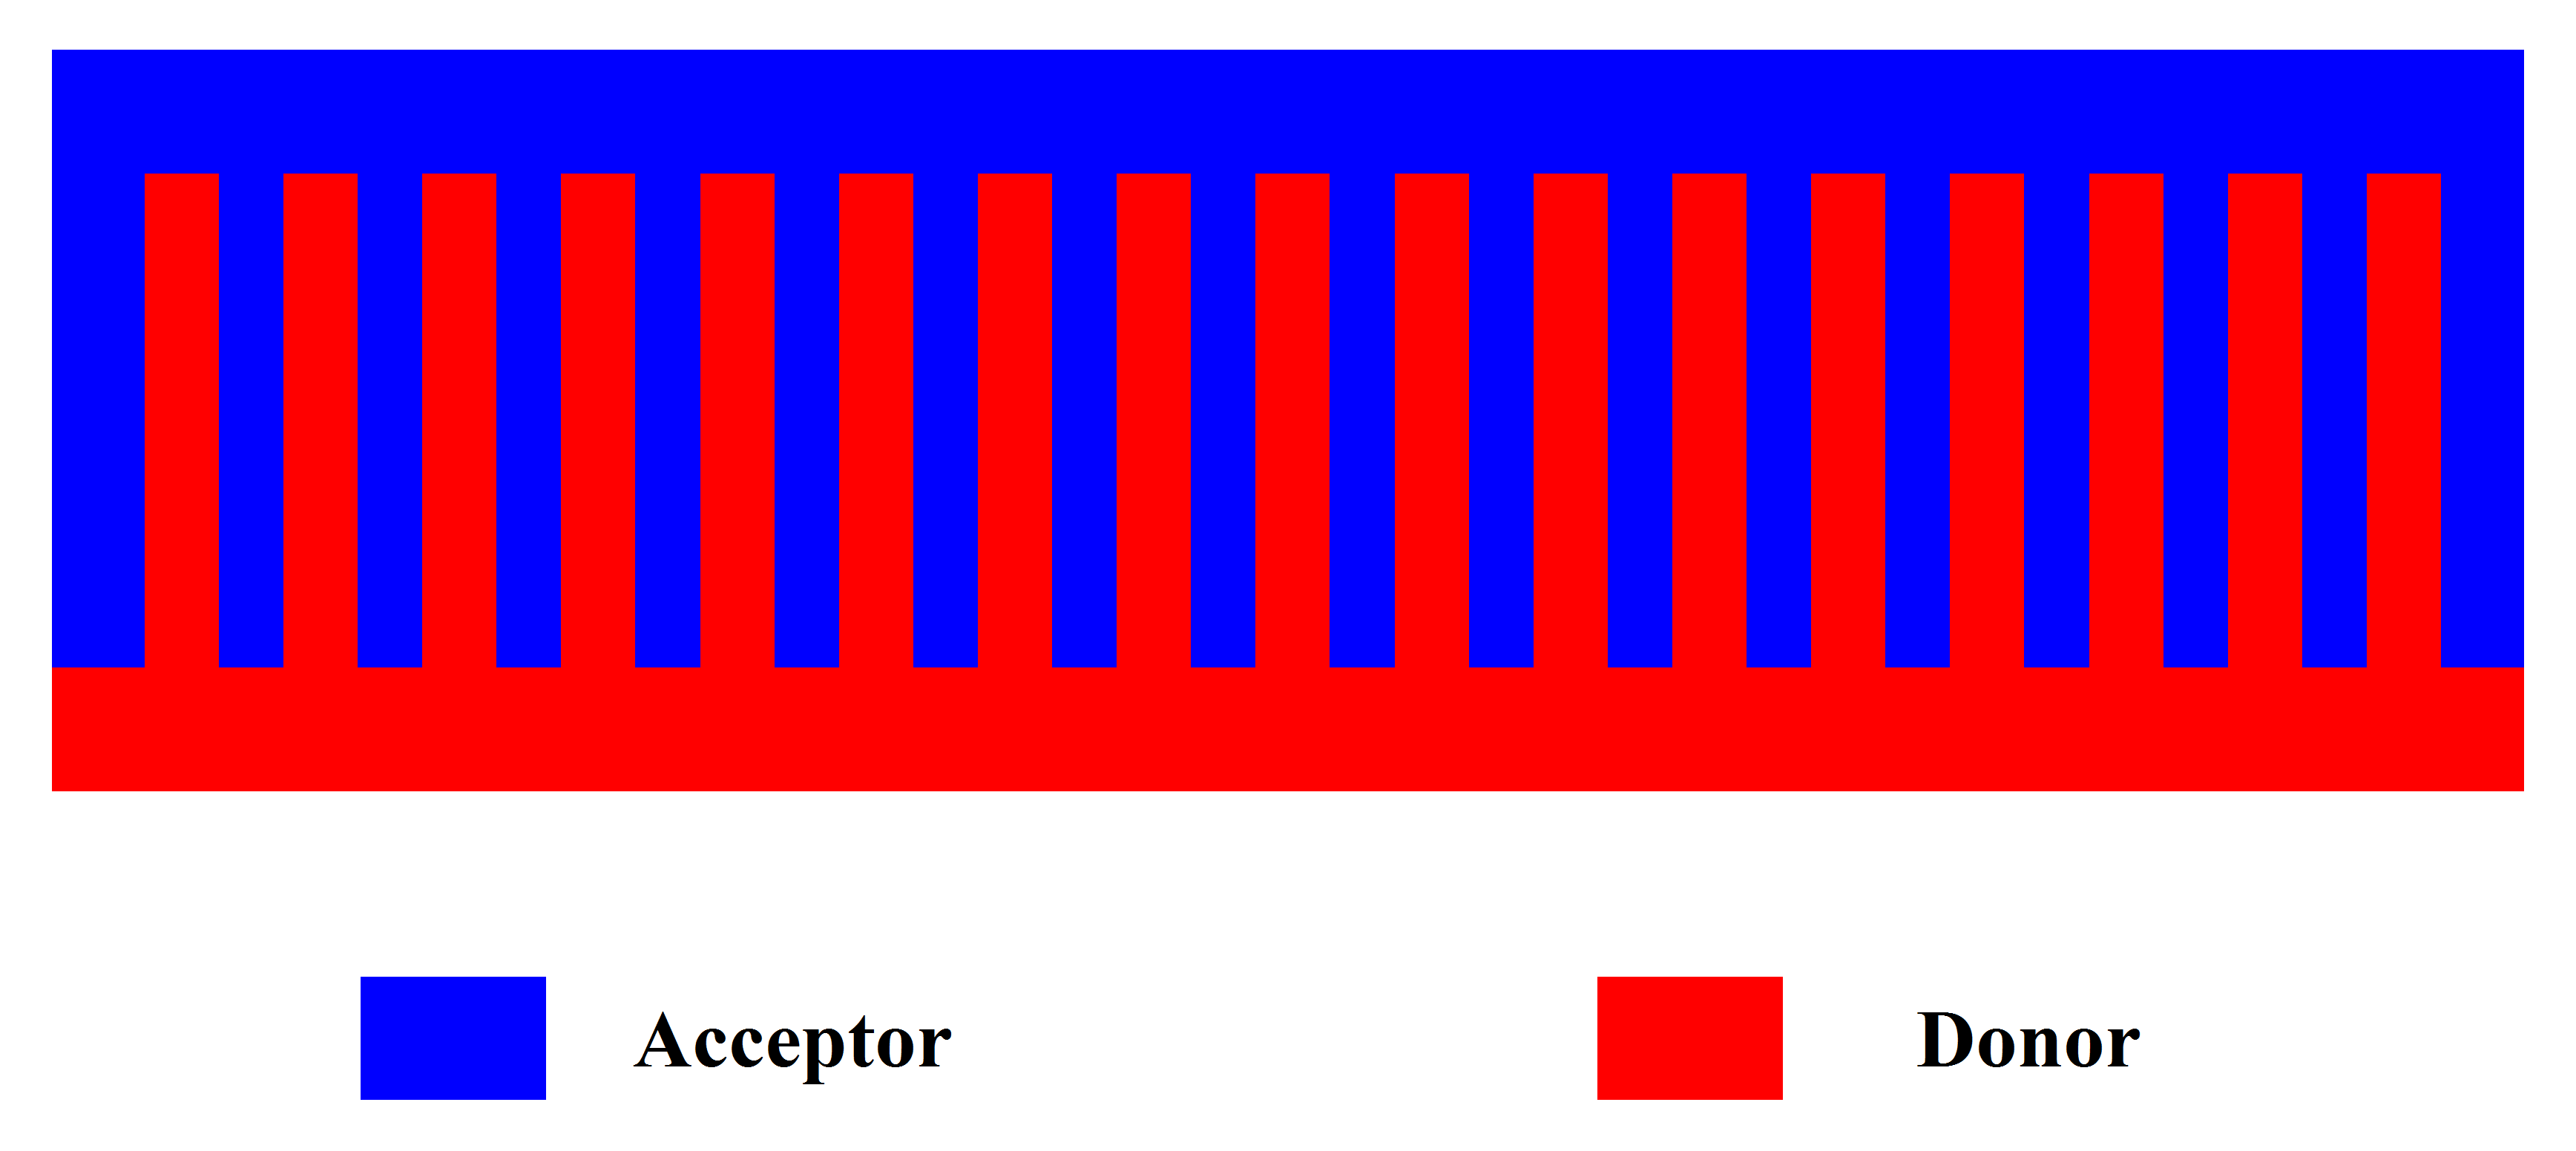
\includegraphics[scale=0.8]{./figures/solar2d.png}
    \caption{理想情况下的有机体异质结太阳能电池的结构}
    \label{fig:solar}
\end{figure}

\begin{figure}[h!]
    \centering
    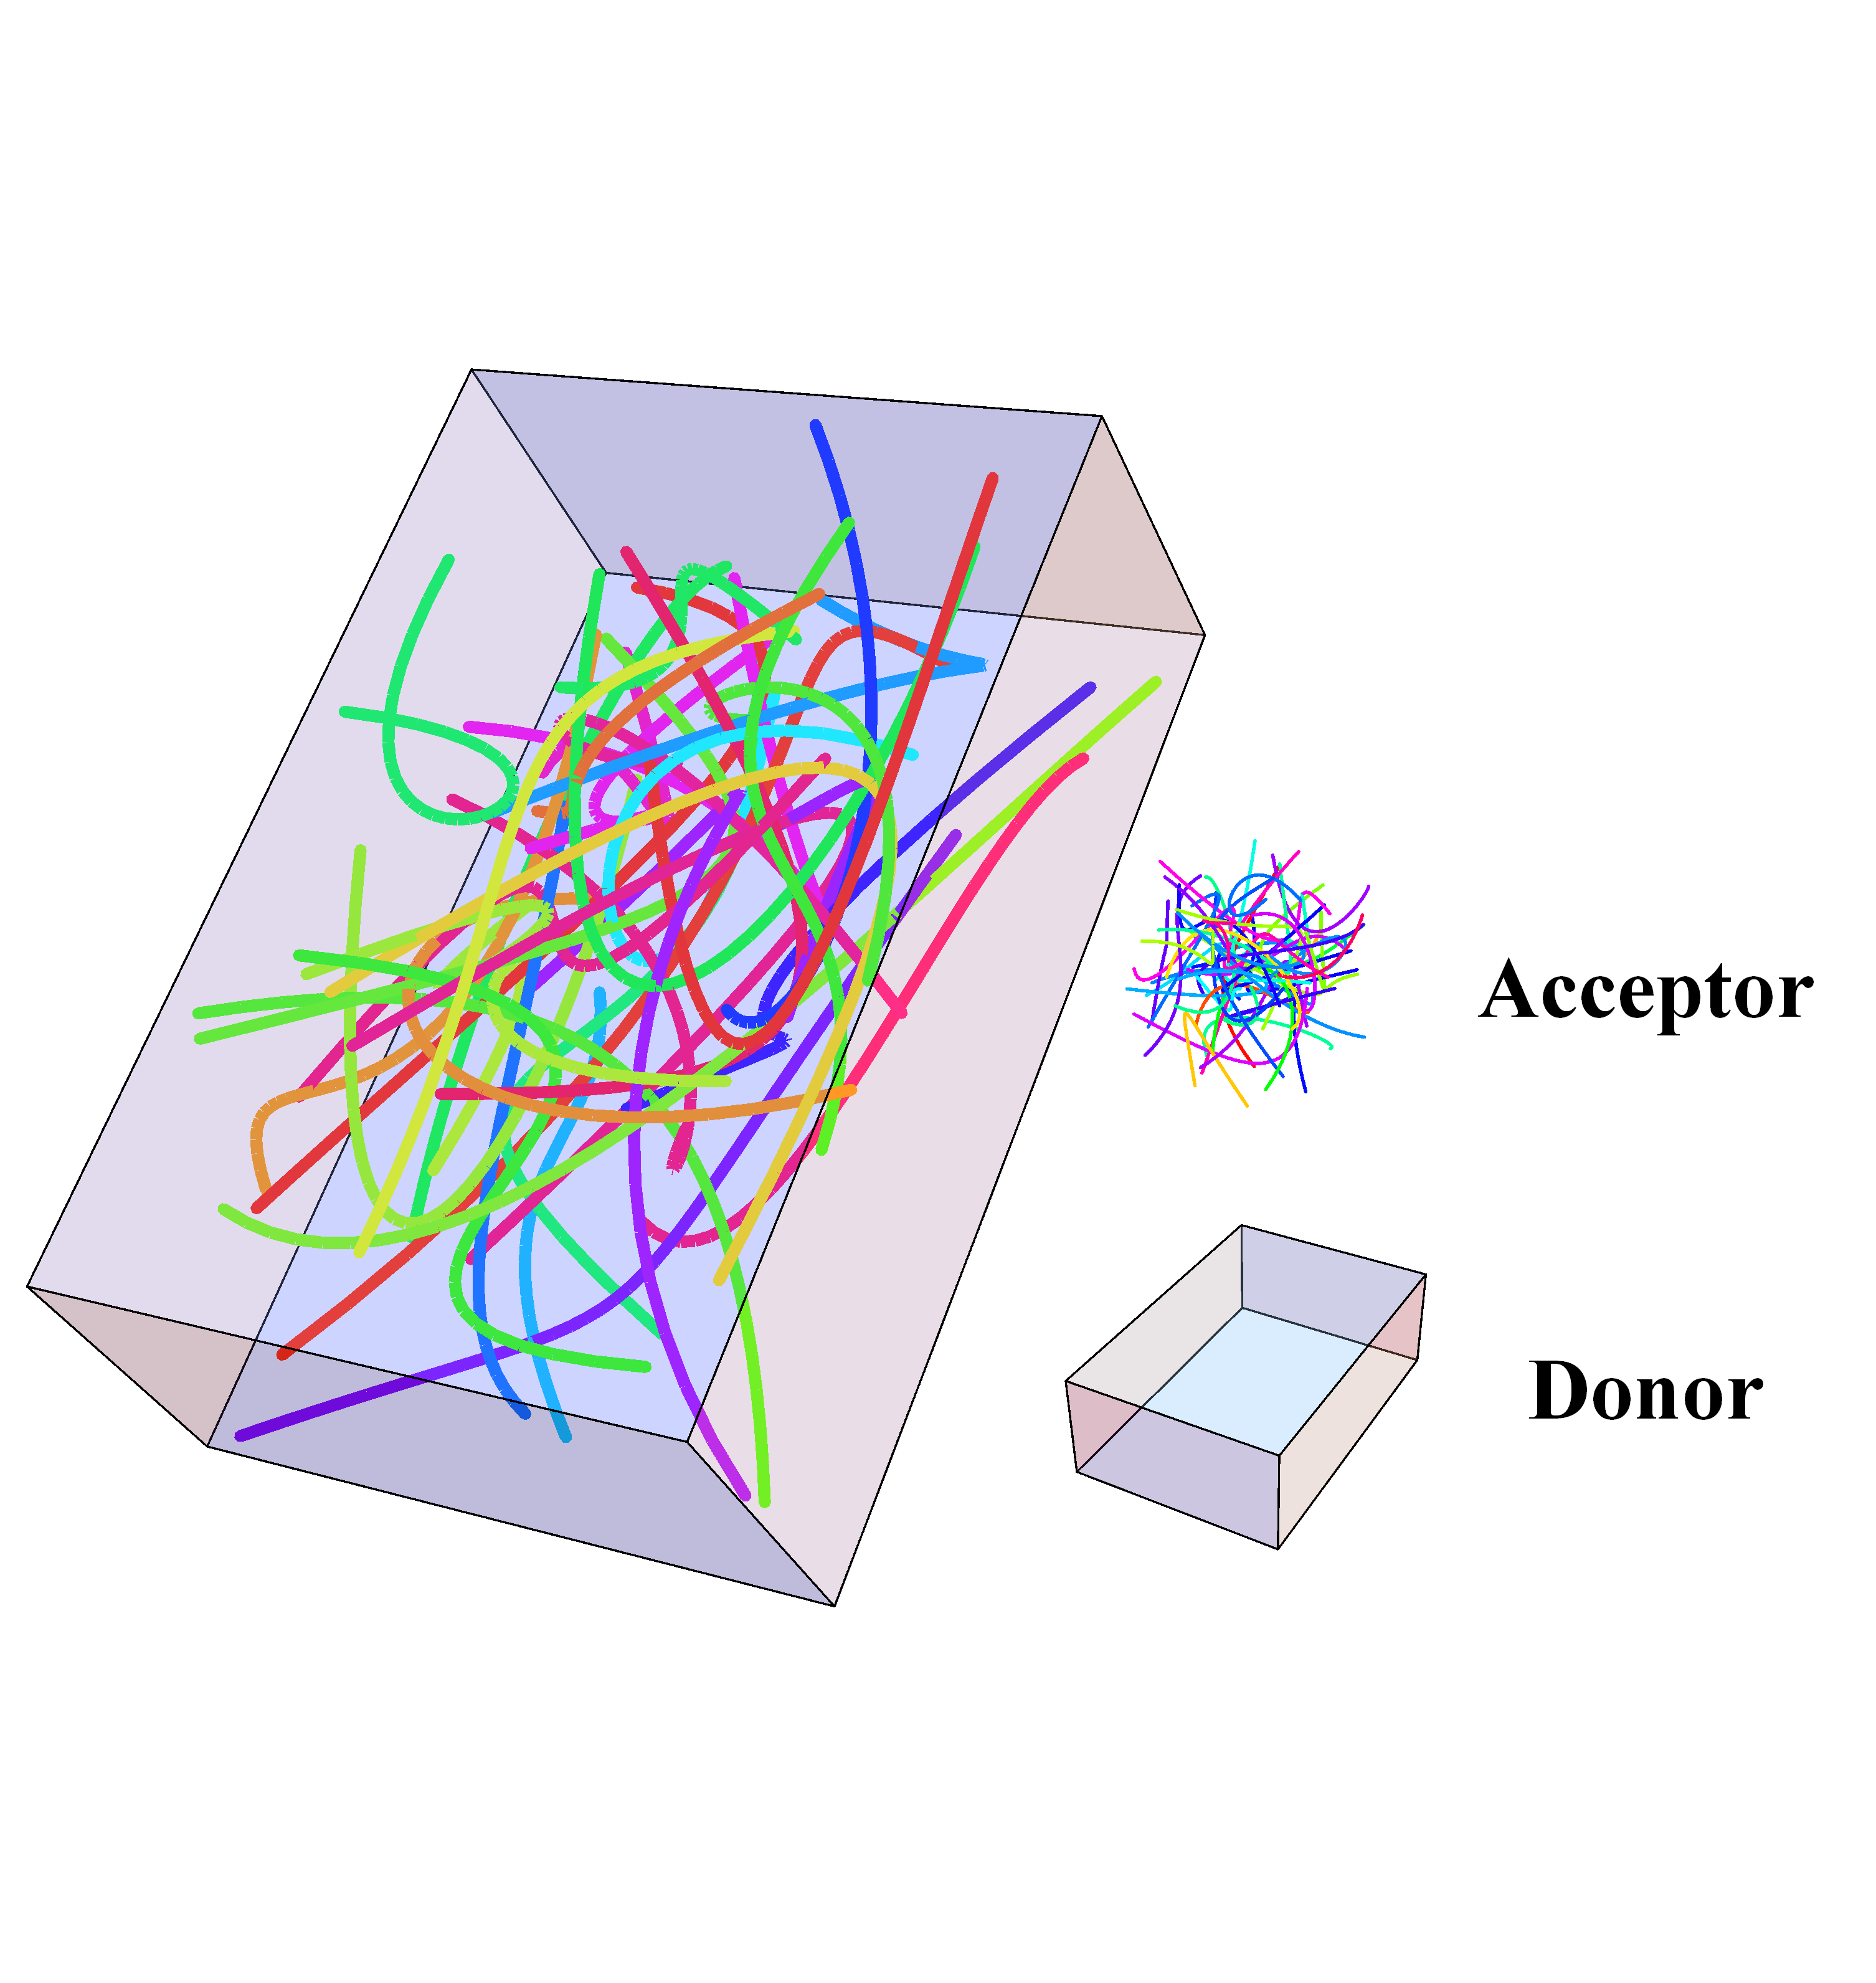
\includegraphics[scale=0.8]{./figures/solar3d.png}
    \caption{现实情况下的有机体异质结太阳能电池的结构}
    \label{fig:solar3d}
\end{figure}

\section{1.3 探究思路}\label{ux63a2ux7a76ux601dux8def}

\subsection{1.3.1
激子形成的研究思路}\label{ux6fc0ux5b50ux5f62ux6210ux7684ux7814ux7a76ux601dux8def}

对于有机异质结太阳能电池而的探究而言,本文将关注其原理中的四个环节里的两个环节:
激子 的形成过程与载流子的输运过程。实验在 MEH-PPV 或者
P3HT的薄膜以及溶液里进行了超快辐射研究并发现激子的自局域过程是一个小于100飞秒超快过
程。\textsuperscript{{[}53{]},{[}54{]}} 但是,与自局域过程相比而言,激子
的形成却是一个相对较为缓慢的过程,大致在1皮秒,即1000飞秒左右。在体异质结太阳能电池
中,激子的局域与形成都发生在给体材料与受
体材料的异质结处。在光激发的条件下,基态电子被激发而形成能带中的电子空穴对。同时,因
为电子与声子的相互作用而在聚合物链中形成局域的激子雏形,在此时,这个电子空穴对
已经发生了分离。为了在理论上阐述激子局域与激子形成,我们将研究激子形成的整个过
程。参考实验中观察到的去极化,光谱红移以及振动结构等现象,可以得到激子的形成过程中
将涉及声子以及相应的弛豫过程。我们猜测正是这个弛豫过程造成了电子
空穴对形成与激子形成的不同步。因此,问题的核心即是对弛豫过程做出动力学描述,并且明确
的区分出它与光激发形成的自局域动力学过程的差别,尤其是在对太阳能电池的探究上。

在方法上,
尽管聚合物链位型在外界光激发下的含时变化可以由传统的分子动力学过程来计算。
但在考虑聚合物链的位型明显变化前,我们必须描述出电子空穴对的超快形成过程。然而,这个
过程涉及到电子受激跃迁导致的电子在分子轨道上的占据数的变化,而聚合物链
体系又是一个电子与声子相互作用明显的体系。并非可以由简单的考虑分子的动力学来计算。本
文将为解决这个理论上的不足提供计算方案。这一方案的依据是在2009年,Devizis
等人提出的
电子跃迁偶极矩很可能在与电子声子耦合下的聚合物链运动有直接的关系。\textsuperscript{{[}55{]}}
因此,作为电
子跃迁直接原因的外界光强将会被引入分子动力学,从而为探究激子形成的过程提供了一套新方
案 。

\subsection{1.3.2
光激发下载流子运动的研究思路}\label{ux5149ux6fc0ux53d1ux4e0bux8f7dux6d41ux5b50ux8fd0ux52a8ux7684ux7814ux7a76ux601dux8def}

对于实际的聚合物体异质结太阳能电池而言,激子分离产生的载流子会沿着聚合物链运动。与理
想形态的有机体异质结太阳能电池相比,体异质结太阳能电池中的载流子输运距离更长。这也意
味着,一维情况下聚合物中载流子的运动对于揭示体异质结太阳能电池的效率将变得非常重要。

考量聚合物链上载流子输运的决定因素时,在实验中已经观察到了载流子输运会受两个因素的影
响:一个是在聚合物链中由于分子线极化导致的单体之间的电荷转移积分;另一个是由减少能量
无序引起。\textsuperscript{{[}56{]}}
但除此以外,是否还存在其它关键的因素对载流子
跃迁有影响?我们考虑这样一个情形:一个正在工作的聚合物体异质结太阳能电池放置在外界
光场下,由于聚合物链的长度比较长,光激发生成的带电载流子在输运过程中,极有可能吸收外界光
子的能量而被激发。上述结果也在最近发表的 P3HT/PC60BM NPs
实验中提到的光激
发导致的NP/电介质界面处电子深度自局域的实验中得到了验证。\textsuperscript{{[}57{]}}
不仅如此
,这个实验中还报道了一种机制,即带电载流子被再激发后将在聚合物链中形成一个更深的晶格
畸变。由此,我们可以看到,探索聚合物链中的带电载流子在外界光激发的条件下如何运动
对于研究聚合物体异质结太阳能的工作效率至关重要。在方法上,我们将同样考虑含时电子
受外界光激发引起的跃迁过程,并结合传统的分子动力学方法,旨在深化外界光激发下的载流子
在有机光伏器件,尤其为探索体异质结太阳能电池中的运动规律提供了一个新的切入点。

\clearpage
\setcounter{equation}{0}

\pagestyle{fancy}

\chapter{共轭聚合物的理论模型与动力学方法}\label{ux5171ux8f6dux805aux5408ux7269ux7684ux7406ux8bbaux6a21ux578bux4e0eux52a8ux529bux5b66ux65b9ux6cd5}

\lhead{} \chead{第二章\quad 有机共轭聚合物的理论模型与动力学方法}
\rhead{}

\section{2.1
共轭聚合物的Su-Schrieffer-Heeger模型}\label{ux5171ux8f6dux805aux5408ux7269ux7684su-schrieffer-heegerux6a21ux578b}

有机共轭聚合物的典型模型是由聚合物分子晶格以及 \(\pi\)
电子所组成,其总能量包括晶格的 能量和电子的能量两个部分。如果有 \(H\)
代表整个聚合物链体系的总能量,\(H_l\) 和 \(H_e\) 代
表晶格部分的哈密顿量和电子部分的哈密顿量,那么有机共轭聚合物链的哈密顿量可以表示为这
两个部分能量之和

\begin{equation}
H = H_l + H_e
\end{equation}

\noindent
其中,晶格部分的能量可以写成晶格所具有的动能 \(H_l^k\) 以及晶格的势能
\(H_l^p\) 之和,

\begin{equation}
H_l = H_l^k + H_l^p
\end{equation}

\noindent
晶格的动能涉及到晶格位移, 记作 \(\bm{u_n}\), 其代表第 n
个晶格距离其平衡位置发生的位移。其移动的速度用该位移表示为

\begin{equation}
\bm{\dot{u}_n} = \frac{\partial \bm{u_n}}{\partial t}
\end{equation}

\noindent
所有晶格的动能之和可以写成

\begin{equation}
T_l = \sum\limits_{n}\frac{M}{2} \bm{\dot{u}_n}^2
\end{equation}

\noindent
考虑所有晶格之间的弹性势能,

\begin{equation}
V_l = \frac{1}{2}\sum\limits_n K (\bm{u_{n+1}} - \bm{u_n})^2
\end{equation}

\noindent
在这里,K代表弹性常量。因此,晶格系统的整体哈密顿量为

\begin{equation}
H_l = \sum\limits_{n}\frac{M}{2} \bm{\dot{u}_n}^2 + \frac{1}{2}\sum\limits_n K
(\bm{u_{n+1}} - \bm{u_n})^2
\end{equation}

我们现在考虑电子部分的哈密顿量\(H_e\)。电子是在以电子声子相互作用的周期势场下运动的。
同样地,我们用第n个晶格位移来表征其对第i个\(\pi\)电子的势能作用。如果原子所在的位置为平
平衡位置,我们设其位移为\(\bm{R_n^{0}}\),它相对于平衡位置移动了\(\bm{u_n}\),那么原子的
新位移位于

\begin{equation}
\bm{R_n} = \bm{R_l^{0}} + \bm{u_l}
\end{equation}

\noindent
我们用\(\bm{r_i}\)代表第i个\(\pi\)电子的位置坐标,\(V(\bm{r_i} - \bm{R_n})\)代表第n个晶格
上的原子对第i个原子上的\(\pi\)电子所作用的势能,那么整个晶格链上的所有原子对该\(\pi\)电
子的势能之和为

\begin{equation}
U(\bm{r_i}) = \sum\limits_n V(\bm{r_i} - \bm{R_n})
\end{equation}

\noindent
如果用\(\bm{p_i}\)代表电子的动量,\(m\)表示电子的质量,那么电子的动能可以表示为

\begin{equation}
T_i = \frac{\bm{p_i}^2}{2 m}
\end{equation}

\noindent
在得到第i个位置上的电子势能以及其动能后,我们将可以把描述该电子的哈密顿量写成

\begin{equation}
H_e(i) = \frac{\bm{p_i}^2}{2 m} + \sum\limits_n V(\bm{r_i} - \bm{R_n})
\end{equation}

\noindent
如果把所有电子的能量相加,我们可以把描述聚合物链上的所有\(pi\)电子的哈密顿量写成

\begin{equation}
H_e = \sum\limits_i H_e(i) = \sum\limits_i [\frac{\bm{p_i}^2}{2 m} + \sum\limits_n
V(\bm{r_i} - \bm{R_n})]
\end{equation}

\noindent
由于原子的质量比电子的质量要大的多,所以其量子效应较小,在哈密顿量中,原子的动量不需
要代换成算符,这就使得原子部分的哈密顿量是经典的。电子部分的哈密顿量则要复杂得多,因
为它的动量必须是替换成算符\(-i\hbar\nabla_i\)。薛定谔方程的解的难度也要大的多。在这里
,我们考虑聚合物链的特点,采适当的近似方法,简化体系的哈密顿量。

在相邻的聚合物单体之间,\(\pi\)电子的电子云(波函数)会互相交叠,因而只有相邻的原子之间
的相互作用需要被考虑,此时的相互作用能我们设为函数
\(-t(\Delta\bm{R_n})\),其中\(\Delta\bm{R_n} = \bm{R_{n+1}} - \bm{R_n}\),函数t是相邻两
个原子之间距离的函数。受此相互作用,\(\pi\)电子可以从某个原子出发,跳向临近的原子。因
此,在聚合物链上,\(\pi\)电子的运动可以被描述为在聚合物单体上的跳跃组成。现在我们来看
\(\pi\)电子的某一次跳跃,即从第n个原子的位置跳向近临的第 n+1
个原子的位置。此时,在第n个 原子的位置上,一个电子消失,而在第 n+1
个位置上增加了一个电子。在量子力学中,这种跳跃 过程可以被``产生算符''
\(a_{n+1}^\dagger\) 与``湮灭算符'' \(a_{n}\) 描述。\(a_{n+1}^\dagger\)
表示在第 n+1 个原子的位置上增加了一个电子,而 \(a_n\)
表示在第n个原子的位置上减少一个电子。那么,当电
子从第n个位置跳向第n+1个位置的过程就可以表示为 \(a_{n+1}^{\dagger}a_n\)
。相反,电子从第 n+1 个原子跳回第 n 个原子的过程是
\(a_{n}^{\dagger}a_{n+1}\) 。发生这种跳跃的几率取决于
相邻两个原子之间的相互作用\(-t(\Delta\bm{R_n})\),其中
\(\Delta\bm{R_n}=\bm{R_{n+1}} - \bm{R_{n}}\)。该相互作用越强,表示跳跃的几率越大。因此,电子的哈密顿量可以写为

\begin{equation}\label{eq:ssh0}
H_e = - \sum\limits_n t(\Delta\bm{R_n})(a_{n+1}^{\dagger} a_{n} + a_n^{\dagger}
a_{n+1})
\end{equation}

\noindent
在这里,略做一点补充:因为电子具有自旋\(S = \pm \dfrac{1}{2}\),为了表示跳跃电子的自旋状态,把产生与湮灭算符写成\(a_{n,s}^\dagger\)和
\(a_{n,s}\),说明在第n个原子上增加或减少了一个自旋为\(s\)的电子。此时,考虑到原子离开平
衡位置\(\bm{R_n^{(0)}}\)的位移非常小,这时候相邻原子间的距离
\(\Delta\bm{R_n}=\bm{R_{n+1}} - \bm{R_{n}} = (\bm{R_{n+1}^{(0)}} - \bm{R_{n}^{(0)}}) + (\bm{u_{n+1}}-\bm{u_n})\)非常接近平衡位置\(\bm{R_{n+1}^{(0)}} - \bm{R_n^{(0)}}\),即
\(\left|\bm{u_{n+1}} - \bm{u_n}\right|\)。因此,我们可以把相互作用的跳跃几率
\(t(\bm{R_{n+1}}-\bm{R_n})\)展开为

\begin{equation}
t(\Delta\bm{R_{n}}) = t_0 - \alpha(\bm{u_{n+1}}-\bm{u_n})
\end{equation}

其中,\(t_0 = t(\Delta\bm{R_n^{(0)}}) = t(\bm{R_{n+1}^{(0)}} - \bm{R_{n}^{(0)}})\),把
该式带入公式(\ref{eq:ssh0}),可以得到哈密顿量

\begin{equation} \label{eq:ssh_e}
H_e = - \sum\limits_{n,s} \Big[ t_0 - \alpha (\bm{u_{n+1}}-\bm{u_n})
\Big](a_{n+1,s}^\dagger a_{n,s} + a_{n,s}^\dagger a_{n+1,s})
\end{equation}

\noindent
此时,整个聚合物链的哈密顿量变为

\begin{equation}
\begin{split}
H & = H_e + H_l \\
  & = -\sum\limits_{n,s} \Big[ t_0 - \alpha (\bm{u_{n+1}}-\bm{u_n})
  \Big](a_{n+1,s}^\dagger a_{n,s} + a_{n,s}^\dagger a_{n+1,s}) \\ 
  &  \quad + \dfrac{K}{2} \sum\limits_n (\bm{u_{n+1}} - \bm{u_n})^2 +
  \dfrac{M}{2}\sum\limits_n \bm{\dot{u}_n}^2
\end{split}
\end{equation}

这个哈密顿量被称为 Su-Schrieffer-Heeger
哈密顿量,简称为SSH哈密顿量。它是由W.P. Su,
Schrieffer和Heeger三个人共同提出来的。\textsuperscript{{[}58{]}}

\noindent
在包含有\(\alpha\)的一项中,同时包括了电子的产生湮灭算符\(a^\dagger\)与\(a\)和晶格运动的位
移\(u\),所以这一项是用来描述晶格原子与电子之间的相互作用。包含\(t_0\)项的只有电子的产生
与湮灭算符,因此,它只表示电子跳跃的能量。哈密顿量最后的两项之包括晶格原子的位移,它
表示的是原子的势能和动能。

此外,补充一下产生与湮灭算符变化为矩阵的对应法则:

\begin{equation} \label{eq:operator}
\begin{split}
& a_m | m \rangle = |0 \rangle \quad
 a_m | 0 \rangle = 0 \\
& a_m^\dagger | 0 \rangle = |m \rangle \quad
 a_m^\dagger | m \rangle = 0 \\
\end{split}
\end{equation}

\noindent
其中的波函数我们用Dirac符号表述,我们做如下规定,\(| n \rangle\)
表示在第n个晶格上有一 个电子,\(| 0 \rangle\)
表示在晶格链对应位置上没有电子。因此,\(a_m | m \rangle = |0 \rangle\)
代表在第m个晶格位置上减少一个电子;\(a_m | 0 \rangle = 0\)
表示在第m个位置上
(本身没有电子的占据)再减小一个电子,这样是不允许的,所以这个变换的值是\(0\)。相反,
\(a_m^\dagger | 0 \rangle = |m \rangle\)表示在原来没有电子占据的第m个位置增加了一个电
子,\(a_m^\dagger | m \rangle = 0\)
表示在有电子占据的第m个位置上再增加一个电子,这是
不允许的,因此这个变换的值也是\(0\)。

\section{2.2
电子本征谱与晶格动力学的计算}\label{ux7535ux5b50ux672cux5f81ux8c31ux4e0eux6676ux683cux52a8ux529bux5b66ux7684ux8ba1ux7b97}

在得到了电子部分与晶格部分的哈密顿量后,我们就要对体系的能量与波函数进行定量的计算。
晶格部分,前面已经提到过,采用``紧束缚近似''的经典处理,但考虑到晶格运动的位移不仅影响
了电子部分的哈密顿量,反过来,电子的能谱和波函数也会决定晶格运动下一时刻的位置和速度
。因此,我们先把焦点放在求解电子部分的能谱和波函数。

参考式
(\ref{eq:ssh_e}),我们必须先对它进行矩阵化:首先,我们对于原子的位移做一个代换,即
\(\bm{u_n} = (-1)^n \bm{\phi_n}\),代换后的物理量\(\phi_n\)代表第n个位置上的位移序参量。然后,对于一维的共
轭聚合物而言,我们把该哈密顿量代入矩阵的表达式

\begin{equation}
\begin{aligned}
\langle m|H_e|n\rangle &=-\sum\limits_{\beta}C^\beta A_{m,n}^\beta \\
C^\beta&=-[t_0+\alpha (-1)^\beta (\bm{\phi_\beta} + \bm{\phi_{\beta + 1}})] \\
A_{m,n}^\beta&=\langle m|a_{\beta+1}^\dagger a_\beta + a_\beta^\dagger
a_{\beta+1}|n \rangle
\end{aligned}
\end{equation}

\noindent
利用关系式(\ref{eq:operator}),我们分别计算出\(\langle m |a_{\beta+1}^\dagger a_\beta| n \rangle\),
\(\langle m |a_{\beta}^\dagger a_{\beta+1}| n \rangle\)

\begin{equation}
\langle m |a_{\beta+1}^\dagger a_\beta| n \rangle=\langle m |a_{\beta+1}^\dagger | \delta(\beta,n) \rangle 
\langle m |a_{\beta}^\dagger a_{\beta+1}| n \rangle=\langle m |a_{\beta}^\dagger | \delta(\beta+1,n) \rangle
\end{equation}

\noindent
其中,

\begin{equation}
| \delta(\beta,n) \rangle=\begin{cases}
|0 \rangle, &  \beta=n\\
0, & \beta\neq n
\end{cases}
\end{equation}

\noindent
我们可以得到,

\begin{equation}
\langle m |a_{\beta+1}^\dagger a_\beta| n \rangle
=\langle m |a_{\beta+1}^\dagger | \delta(\beta,n) \rangle
=
\begin{cases}
    \langle m | n + 1 \rangle, & \beta = n \\
    0, & \beta \neq  n
\end{cases}
\end{equation}

\begin{equation}
\langle m |a_{\beta}^\dagger a_{\beta+1}| n \rangle
=\langle m |a_{\beta}^\dagger | \delta(\beta+1,n) \rangle
=
\begin{cases}
    \langle m | n - 1 \rangle, & \beta + 1 = n \\
    0, & \beta + 1 \neq  n
\end{cases}
\end{equation}

\noindent
因此, 数值上来说,\(H_e\) 将变成

\begin{equation} \label{eq:dig_H_e}
\begin{split}
\langle m | H_e | n \rangle
 &=\sum\limits_{\beta}C^\beta A_{m,n}^\beta \\
 &=
\begin{cases}
    C_n=-[t_0+(-1)^n(\bm{\phi_n}+\bm{\phi_{n+1}})], & m = n +1\\
    C_{n-1}=-[t_0+(-1)^{n-1}(\bm{\phi_{n-1}}+\bm{\phi_n})], & m = n - 1
\end{cases}
\end{split}
\end{equation}

\noindent
在得到该\(H_e\)的矩阵形式后,我们可以通过对该矩阵对角化而得到聚合物中电子运动的本征能
谱和本征波函数。

在得到电子哈密顿量对应矩阵\(\langle \mu | H_e | \nu \rangle\)之后,
我们就可以得到该电
子在聚合物中运动的本征波函数\(\langle \mu | \Psi^k \rangle\),其中
\(k = 1, 2, ...\)。
同时,本征能谱中的第n个能级也可以被得到,记作\(\varepsilon^k\)。我们把该哈密顿量的矩阵
形式带入到薛定谔方程中

\begin{equation}
H_e | \Psi^k \rangle = \varepsilon^k | \Psi^k \rangle
\end{equation}

\noindent
其中,我们把描述电子在聚合物链中的运动用波函数\(| \Psi^k \rangle\)表示,现在我们把该方
程矩阵化:首先,我们用电子本征矢量 \(| m\rangle\)
左乘在等式两边做内积得到

\begin{equation} \label{eq:dig_ssh}
\langle m | H_e | \Psi^k \rangle = \varepsilon^k \langle m | \Psi^k \rangle
\end{equation}

\noindent
此时,展开波矢\(| \Psi^k \rangle\) 为
\(| \Psi^k \rangle = \sum\limits_n |n \rangle \langle n | \Psi^k \rangle\),则有式(\ref{eq:dig_ssh})变为

\begin{equation} \label{eq:dig_ssh2}
\sum\limits_n \langle m | H_e | n \rangle \langle n | \Psi^k \rangle =
\sum\limits_{n'} \varepsilon^k \langle m | n' \rangle \langle n' | \Psi^k \rangle
\end{equation}

\noindent
我们把式(\ref{eq:dig_H_e})代入到式(\ref{eq:dig_ssh2})中,利用正交归一关系得到

\begin{equation} 
C_{m-1} \langle m - 1 | \Psi^k \rangle + C_{m+1} \langle m + 1 | \Psi^k \rangle = 
\varepsilon_k \langle m | \Psi^k \rangle
\end{equation}

\noindent
我们把Dirac符号重新用普通函数记号来表示:\(\mathcal{Z}_m^k \equiv \langle m | \Psi^k \rangle\),那么上式将变为

\begin{equation} \label{eq:dig_ssh3}
C_{m-1} \mathcal{Z}_{m-1}^k + C_{m+1} \mathcal{Z}_{m+1}^k = \varepsilon_k
\mathcal{Z}_m^k
\end{equation}

这里,我们可以考虑某时刻聚合物链体系的位移序参量\(\bm{\phi_n} (n = 1, 2, ...)\)在
\(\Delta T\)时间段之后的状态\(\bm{\phi_n^{t+1}} (n = 1, 2, ...)\)。通过对经典的牛顿运动方程进行运算,我们可以知道
:假设在质点群中有一个标记为第n个的质点,它的位置为\(\bm{x_n^t}\),速度为\(\bm{v_n^t}\),
质量为\(M_n\)。并同时假设,在此时刻,该质点在势场\(U(\bm{x_n^t})\)中运动,因此该质点将受
到\(\bm{F_n^t} = - \dfrac{\delta U(\bm{x_n^t})}{\delta \bm{x_n^t}}\)的作用。从该时刻起,该质
点的运动方程即为

\begin{equation}
\begin{aligned}
\bm{x_n^{t+1}} &= \bm{x_n^t} + \bm{v_n^t} \Delta T \\
\bm{v_n^{t+1}} &= \bm{v_n^t} + \dfrac{\bm{F_n^t}\Delta T}{M_n} 
\end{aligned}
\end{equation}

\noindent
类似的,我们将其中的\(\bm{x_n^t}\)代换成为\((-1)^n \phi_n^t\)即可以得到晶格位移序参量的
含时演化,

\begin{equation}
\begin{aligned}
\bm{\phi_n^{t+1}} &= \bm{\phi_n^t} + (-1)^n\bm{v_n^t} \Delta T \\
\bm{v_n^{t+1}} &= \bm{v_n^t} + \dfrac{\bm{F_n^t}\Delta T}{M_n} 
\end{aligned}
\end{equation}

\noindent
其中,对于一维的有机共轭聚合物体系,上述表达式中的力\(F_n\)可由Feynman-Hellmann定理
求得

\begin{equation}
\begin{split}
F_n &= - \langle \Psi | \dfrac{\partial H}{\partial \phi_n} | \Psi \rangle \\
&=
\begin{cases}
2 \alpha \displaystyle \sum\limits_s W_{0,s} - K (\phi_0 + \phi_1) - K' \alpha, & n = 0 \\
2 \alpha \displaystyle \sum\limits_s W_{N-2,s} - K (\phi_{N-2} + \phi_{N-1}) - K' \alpha, & n = N-1 \\
2(-1)^n \alpha \displaystyle \sum\limits_s (W_{n,s}-W_{n-1,s}) - K (\phi_{n-1} + 2 \phi_{n} +
\phi_{n+1}) - K' \alpha, & 0 < n < N-1 
\end{cases}
\end{split}
\end{equation}

\noindent
上式中的\(W_{n,s} = \displaystyle \sum\limits_\mu Z_{n+1,s}^\mu Z_{n,s}^\mu\),
\(K' = \dfrac{2}{N} \displaystyle \sum\limits_{n,s}\sum\limits_\mu Z_{n+1,s}^\mu Z_{n,s}^\mu\),
其中\(\mu\)是能级的指标,\(n\)是位置的指标,\(s\)是电子自旋的指标。

\section{2.3
占据态的电子与晶格的耦合方程}\label{ux5360ux636eux6001ux7684ux7535ux5b50ux4e0eux6676ux683cux7684ux8026ux5408ux65b9ux7a0b}

首先,我们利用电子部分的哈密顿量,可以得到电子在聚合物链体系下的本征能谱和本征波函数
。然后,我们利用经典牛顿力学得到了晶格的位移序参量含时演化的方程。但是,考虑到电子和
晶格的相互作用,即在某一时刻的电子的本征能谱与本征波函数将和该时刻的晶格位移有函数关
系,该关系直接影响了有电子实际占据情况下的晶格位移的运动方程。因此,我们需要关注在一
个聚合物链体系中占据态的电子晶格耦合方程。假设我们对所有被占据能级的能量取和

\begin{equation} \label{eq:E_e}
E_{\mu} = \sum\limits_i^{\mu} \varepsilon_i
\end{equation}

\noindent
\(\mu\)表示占据态的个数。我们把电子占据能量与晶格原子的能量求和,就可以得到体系的总能量

\begin{equation} \label{eq:E_el}
E = E_{\mu} + \frac{K}{2}\sum\limits_i (\bm{u_{i+1}} - \bm{u_i})^2 + \frac{M}{2}
\sum\limits_i \bm{\dot{u}_i}
\end{equation}

\noindent
考虑到体系必须要处于极小值状态才能使得晶格的位移序参量达到稳定,即具有稳定的位型。因
此,对第i个位置的晶格原子,我们有方程

\begin{equation} \label{eq:var_cal}
\dfrac{\delta E(\bm{u_i})}{\delta \bm{u_i}} = 0 \quad (i = 1, 2, ...)
\end{equation}

\noindent
我们将式(\ref{eq:dig_ssh3}),式(\ref{eq:E_e}),式(\ref{eq:E_el})带入式(\ref{eq:var_cal})中,可以得到

\begin{equation}
\bm{u_{i+1}} - \bm{u_i} = -\dfrac{2 \alpha}{K} \Big[ \sum\limits_k \mathcal{Z}_i^k
\mathcal{Z}_{i+1}^k - \dfrac{1}{N} \sum\limits_{i'}\sum\limits_k \mathcal{Z}_{i'}^k 
\mathcal{Z}_{i'+1}^k\Big]
\end{equation}

\noindent
其中,\(N\)表示聚合物链体系由\(N\)个聚合物单体组成。

\section{2.4
电子间相互作用Hatree-Fock近似}\label{ux7535ux5b50ux95f4ux76f8ux4e92ux4f5cux7528hatree-fockux8fd1ux4f3c}

电子之间的相互作用在强关联体系中必须考虑。有机半导体聚合物材料中,整个能带宽度约为\(10 eV\),但是此类材料的电子间相互作用一般都不大于\(5eV\),所以该体系不属于强关联体系。也因
为如此,电子的相互作用在此范围内对电子的运动性质并不会带来显著的变化。所以,我们在描
述电子间相互作用对体系哈密顿量的影响时,采用在SSH模型中加入扩展的Hubbard项,再利用
Hatree-Fock近似来得到此相互作用。经过Hubbard模型修正后的哈密顿量为

\begin{equation}
H = H_{ssh} + H_{e-e}
\end{equation}

\noindent
其中,\(H_{e-e}\)为电子与电子的相互作用

\begin{equation}
\begin{split}
H_{e-e} &= \dfrac{U}{2} \sum\limits_{n,s} \Big( a_{n,s}^\dagger a_{n,s} -
\dfrac{1}{2} \Big)\Big( a_{n,-s}^\dagger a_{n,-s} - \dfrac{1}{2} \Big) \\
&\quad + V \sum\limits_{n,s,s'} \Big( a_{n,s}^\dagger a_{n,s} - \dfrac{1}{2}
\Big)\Big( a_{n+1,s'}^\dagger a_{n+1,s'} - \dfrac{1}{2} \Big) 
\end{split}
\end{equation}

\noindent
其中,\(U\) 和 \(V\)
是Hubbard项,分别表示同一个晶格格点上自旋相反电子的相互作用和相邻格点上的电子相互作
用。再做Hatree-Fock近似后的哈密顿量可以表示为

\begin{equation}
\begin{aligned}
H_{e-e} &= \sum\limits_{n,s}\Big\{U\Big( \sum\limits_{\mu} \Big|
\mathcal{Z}_{n,-s}^{\mu} \Big| - \dfrac{1}{2} \Big) \\
&+ V\Big[ \sum\limits_s \Big(
\sum\limits_k \Big| \mathcal{Z}_{k-1,s}^{\mu} \Big|^2 + \sum\limits_{\mu} \Big|
\mathcal{Z}_{n+1,s}^{\mu} \Big|^2 - 2\Big) \Big] \Big\} a_{n,s}^\dagger a_{n,s}\\
&- \sum\limits_{n,s} \Big( V \sum\limits_{k}^{\mu} \mathcal{Z}_{n,k}^{\mu}
\mathcal{Z}_{n+1,k}^{\mu} \Big) (a_{n+1,s}^\dagger a_{n,s} + a_{n,s}^\dagger
a_{n+1,s}) 
\end{aligned}
\end{equation}

\noindent
在把Hatree-Fock近似加入SSH模型之后,可得到Hubbard-SSH模型的电子波函数

\begin{equation}
\begin{aligned}
\varepsilon_s^\mu \mathcal{Z}_{n,s}^\mu &= \Big[ U \Big( \rho_{n,-s} - \dfrac{1}{2} 
\Big) + V \Big(\sum\limits_{s'} \rho_{n-1, s'} + \sum\limits_{s'} \rho_{n+1,s'} -
2\Big) \Big]\mathcal{Z}_{n,s}^{\mu} \\
&- \Big[ V \sum\limits_{\mu} \mathcal{Z}_{n,s}^{\mu} \mathcal{Z}_{n-1,s}^{\mu} 
+ t_0 + \alpha (\bm{u}_{n-1} - \bm{u}_n) + (-1)^{n-1} t_e
  \Big]\mathcal{Z}_{n-1,s}^\mu \\
&- \Big[ V \sum\limits_{\mu} \mathcal{Z}_{n,s}^{\mu} \mathcal{Z}_{n+1,s}^{\mu} + t_0
+ \alpha (\bm{u}_{n+1} - \bm{u}_n) + (-1)^{n+1} t_e \Big] \mathcal{Z}_{n+1,s}^{\mu}
\end{aligned}
\end{equation}

\noindent
其中,电荷分布可以用
\(\rho_{n,s} = \displaystyle\sum\limits_{\mu} \big| \mathcal{Z}_{n,s}^{\mu} \big|\)

\section{2.5
共轭聚合物中电子跃迁的偶极矩计算}\label{ux5171ux8f6dux805aux5408ux7269ux4e2dux7535ux5b50ux8dc3ux8fc1ux7684ux5076ux6781ux77e9ux8ba1ux7b97}

在外界光作用下,电子会被激发而跃迁,这里我们需要考虑电子跃迁的速率。如果我们把能带中
靠近导带的局域能级记作\(\Gamma_u\),用波矢\(|u\rangle\)表示,且该能级上的电子占据数用
\(P_U\)表示;靠近价带的局域能级记作\(\Gamma_d\),用波矢\(|d\rangle\)表示,且该能级上的电子占
据数用\(P_d\)表示。因此,跃迁能级之间的电偶极矩为\(p = P_u \langle u | r | d \rangle\),
其中\(r\)是电偶算符。那么,跃迁速率的表达式为

\begin{equation}
\begin{aligned}
\gamma_{ud} &= \dfrac{4(E_u-E_d)^3}{3\hbar^4c^3} p^2 \\
            &= \dfrac{4(E_u-E_d)^3}{3\hbar^4c^3} \big( P_u \langle u | r | d
            \rangle\big)^2
\end{aligned}
\end{equation}

其中,

\begin{equation}
\begin{aligned}
&\dfrac{dP_u}{dt} = -\gamma_{ud}P_u\\
&P_d = n - P_u
\end{aligned}
\end{equation}

将该跃迁速率方程引入电子的动力学方程,即可探究激发下的电子动力学过程。

\clearpage

\pagestyle{fancy}

\chapter{半导体聚合物中的激子形成}\label{ux534aux5bfcux4f53ux805aux5408ux7269ux4e2dux7684ux6fc0ux5b50ux5f62ux6210}

\lhead{} \chead{第三章\quad 有机半导体聚合物中的激子形成} \rhead{}

具体来说,我们选定一个具有200个单体组成的一维聚合物链。在没有受到外界光强激发下,聚
合物链会在能带中的导带与价带之间形成了一个如图(\ref{fig:unexcited})所示的带隙。

\begin{figure}[h!] 
    \centering
    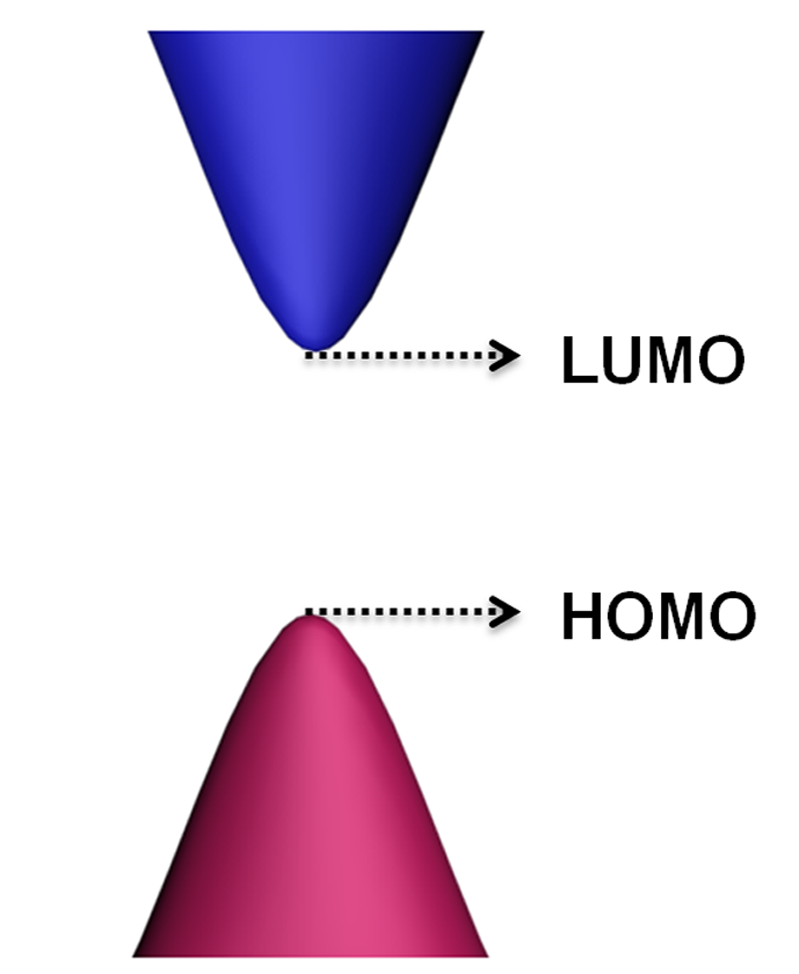
\includegraphics[scale=1]{./figures/Exciton_Figure_1.png}
    \caption{聚合物链在未受光激发的启发下形成的能带}
    \label{fig:unexcited}
\end{figure}

这里,为了描述晶格的位型,在基于聚合物链上第\(n\)个单元上的位移量\(u_n\)的基础上,我们作
如下变换\(\phi_n = (-1)^n u_n\)使得之后的晶格位型以一种平滑的方式呈现。在不受外界光积
光激发的影响下,晶格位型主要表现为单双键之间交替轮流,此为二聚化的结果,如图
(\ref{fig:config})。

\begin{figure}[h!] 
    \centering
    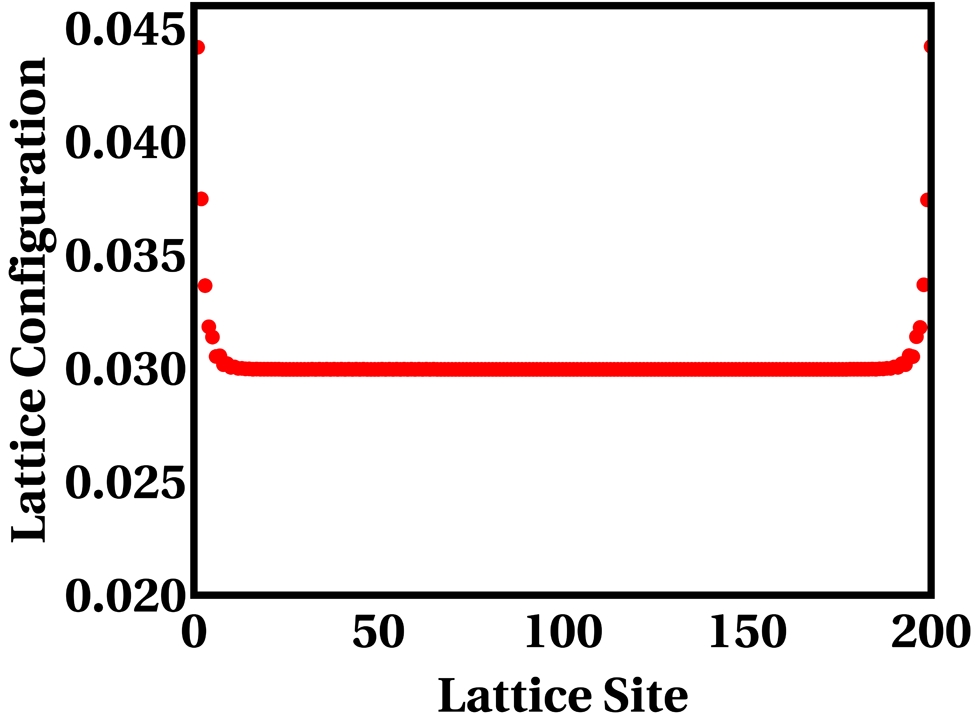
\includegraphics[scale=1]{./figures/Exciton_Figure_2.png}
    \caption{聚合物链未受光激发下的启发下形成的位型}
    \label{fig:config}
\end{figure}

\section{3.1
电子空穴对的局域}\label{ux7535ux5b50ux7a7aux7a74ux5bf9ux7684ux5c40ux57df}

有机共轭聚合物太阳能电池在外界光激发的作用下,如果当外界光的能量与构成有机共轭聚合物
太阳能电池的聚合物材料能隙匹配,HOMO上的电子将被激发到LUMO上去,形成所谓的单线态激子
。在最近的研究中,为了在共轭聚合物以形成激子,A.J.
Heeger实验组分别利用了\(10\mu J/cm^2\),\(20\mu J/cm^2\),\(30\mu J/cm^2\),\(40\mu J/cm^2\)
,四种的外界光来激发共轭聚合物。实验发现,单线态激子的局域和激子的形成两者并不同步。
为了探寻造成两者不同的原因,我们利用第三章提供的方法来刻画单线态激子的局域和形成过程
。此外,我们将从晶格原子位型的演变,电子占据数变化,和电子在空间的分布三个角度来细致
的刻描述个过程。

如最近报告的实验所提供的结果,我们选用\(30\mu J/cm^2\)的外界激光激发共轭
.
聚合物材料。随着外界光场的对共轭聚合物的激发,描述聚合物的晶格畸变状况的晶格位型展示
出不同于二聚化基态的行为,如下图(\ref{fig:evo_config})。

\begin{figure}[h!] 
    \centering
    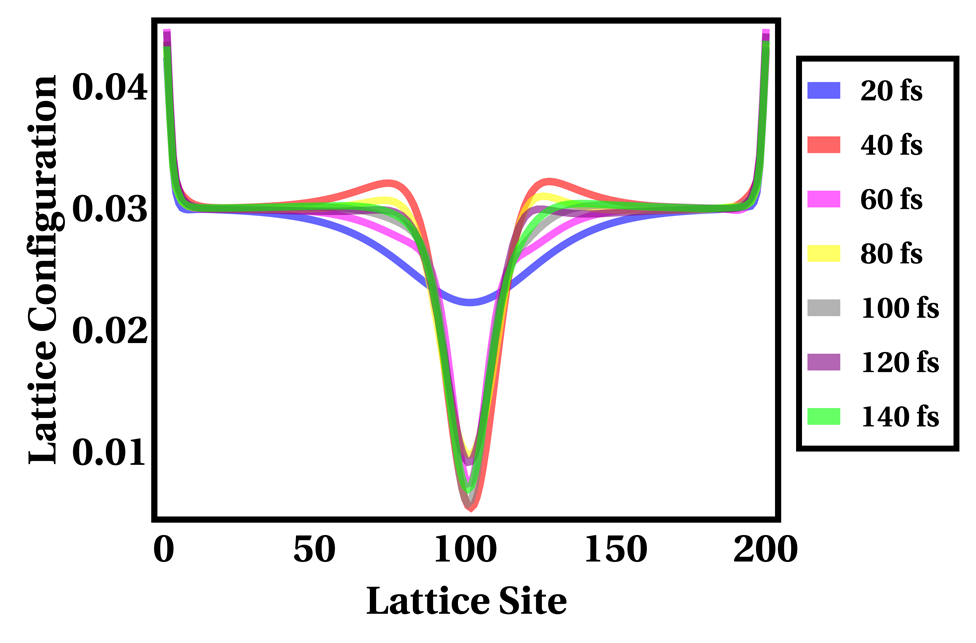
\includegraphics[scale=1]{./figures/Exciton_Figure_3.png}
    \caption{晶格位型在140飞秒内的含时变化}
    \label{fig:evo_config}
\end{figure}

根据最近的实验所应用的外界光强,我们在模拟中对共轭聚合物分子施加\(30\mu J/cm^2\)
的激光,在20飞秒的时候,原本均匀的二聚化基态开始形成了一个浅浅的凹陷。并且,随着激发
过程的演化,在20飞秒到140飞秒之间,局域于共轭聚合物分子链正中的晶格畸变逐渐变强。直
到140飞秒,可以从图 (\ref{fig:evo_config})
的晶格位形中判断,在共轭聚合物分子链的中心,晶格位型发生畸变并形成局域。共轭聚合物分
子晶格畸变的同时,也伴随着共轭聚合物分子在\(30\mu J/cm^2\)的激光激发下电子跃迁的过程。
如果\(30\mu J/cm^2\)
激光的光子能量恰好能符合导带和价带之间产生的能隙,价带上的电子将吸收激发光光子的能量
,跃迁至导带上,从而改变在HOMO和LUMO上电子的占据数。如图(\ref{fig:pop})所示,

\begin{figure}[h!] 
    \centering
    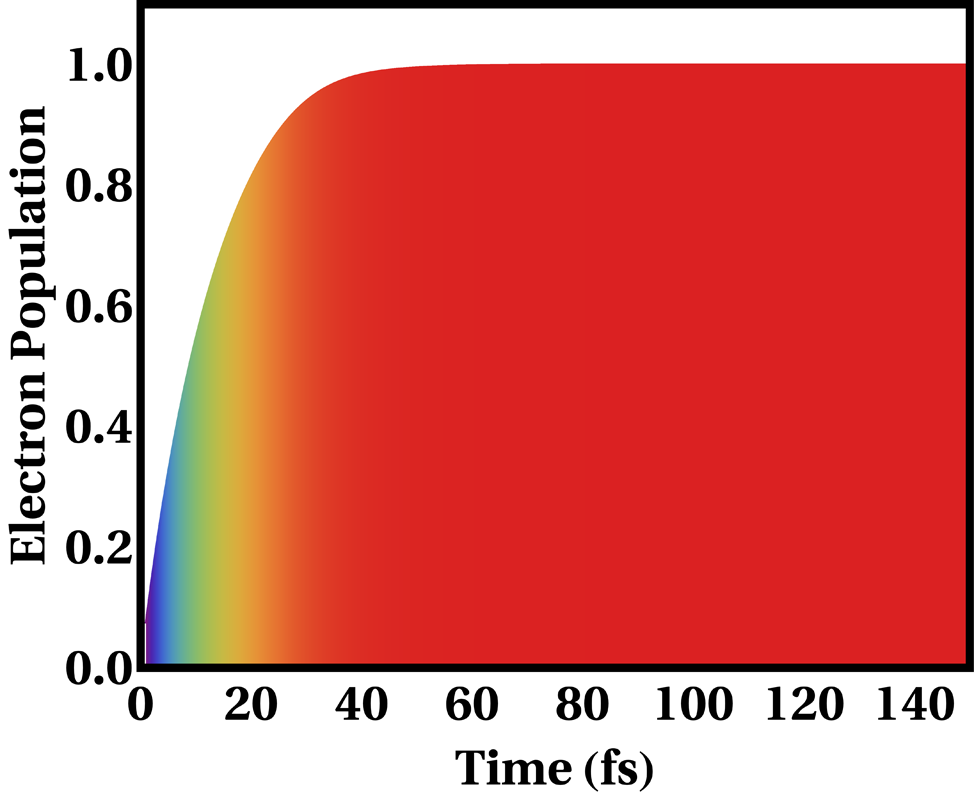
\includegraphics[scale=1]{./figures/Exciton_Figure_5.png}
    \caption{LUMO上的电子占据数在150飞秒内的含时变化}
    \label{fig:pop}
\end{figure}

由于外界光的激发,在50飞秒的时间内,
HOMO上的电子激发至LUMO能级。其中,在\(30\mu J/cm^2\)
外界光激发的初始时间25飞秒内,LUMO上的电子占据数快速的增加,此后,LUMO上的电子占据数开
始缓慢的增加。直到64飞秒,将LUMO能级上的电子占据数接近1。最后,在50飞秒以后
,各能级上电子占据数稳定。正如图
(\ref{fig:pop})所显示的,由此也产生了我们需要解答的一个问题:在\(30\mu J/cm^2\)
外界光激发共轭聚合物材料的开始到50飞秒的时间段,随着电子从HOMO跃迁,LUMO电子增加了,而
在50飞秒以后电子占据数已经稳定的情况下,其状态将如何发生变化?

\begin{figure}[h!] 
    \centering
    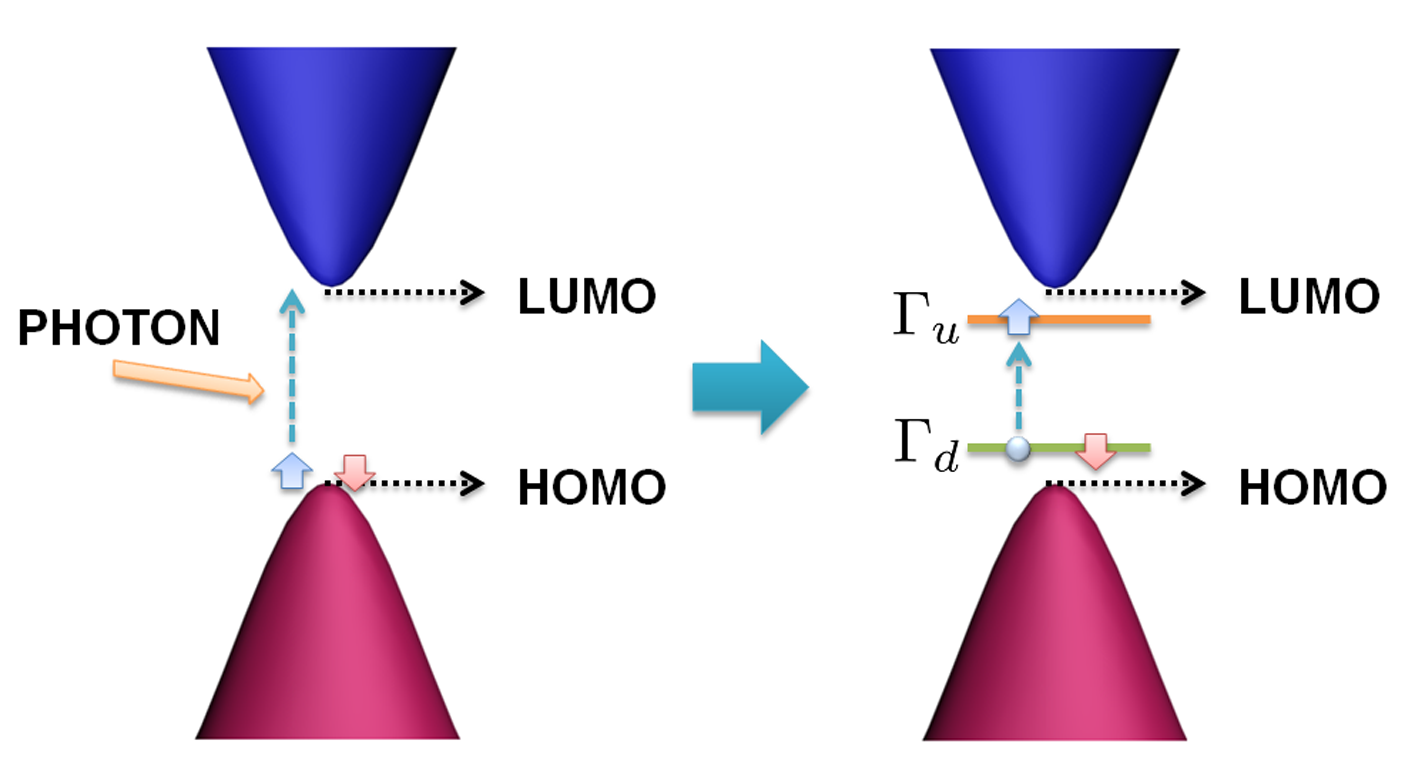
\includegraphics[scale=1]{./figures/Exciton_Figure_4.png}
    \caption{聚合物链中局域能级形成的示意图}
    \label{fig:energy}
\end{figure}

对于这个问题,我们需要考虑到共轭聚合物中较强的电子-声子相互作用,很自然将关注点转移
到电子的空间行为上来。首先我们关注\(30\mu J/cm^2\)
外界光激发共轭聚合物后整个电子能谱的变化。由于电子-声子相互作用,电子状态的变化势必
受到晶格的畸变影响,这包括能谱和电子在空间的分布。 图(\ref{fig:energy})
,正是显示了共轭聚合物分子受激后,HOMO上的电子被激发至LUMO能级上后,原先的HOMO能级
与LUMO能级逐渐向能隙中心移动。结合新的电子占据,原先的HOMO和LUMO逐渐演化成了构成新的
激子的两个新状态,\(\Gamma_u\)和\(\Gamma_d\),它们用来描述构成新激子的电子状态和空穴状态
。而上述的电子能谱和
晶格的变化,也使构成新激子的电子状态发生改变。图(\ref{fig:wavefun})正是刻画在时间尺度上电子在共轭聚合
物分子链上的分布。可以清晰的得到,在\(30\mu J/cm^2\)外界光激发的初始10飞秒,电子从HOMO开
始跃迁至 LUMO,
构成激子的电子是扩展态。但20飞秒后,电子开始被局域于共轭聚合物分子链的中间。随着外界
光激发的继续, 电子的局域态越来越明显,直至50飞秒左右 ,
电子的局域态开始形成。结合晶格在时间尺度上的演化,可以发现光诱发形成激子的过程中,晶
格的局域现象和电子的局域过程恰能相互对应,以上两者恰恰形成了激子的局域。结合图
(\ref{fig:pop}),图(\ref{fig:energy})和图 (\ref{fig:wavefun})
可以发现,外界光激发诱导激子晶格局域,构成激子态的电子局域,恰恰与外界光诱导电子从初
始的HOMO跃迁至LUMO后电子占据数的稳定所需的时间趋于一致,是50飞秒,与最近实验结果一致。
但由此也产生了新的问题:外界激发光的强度是否将直接影响激子晶格局域和电子态局域所需
的时间?

\begin{figure}[h!] 
    \centering
    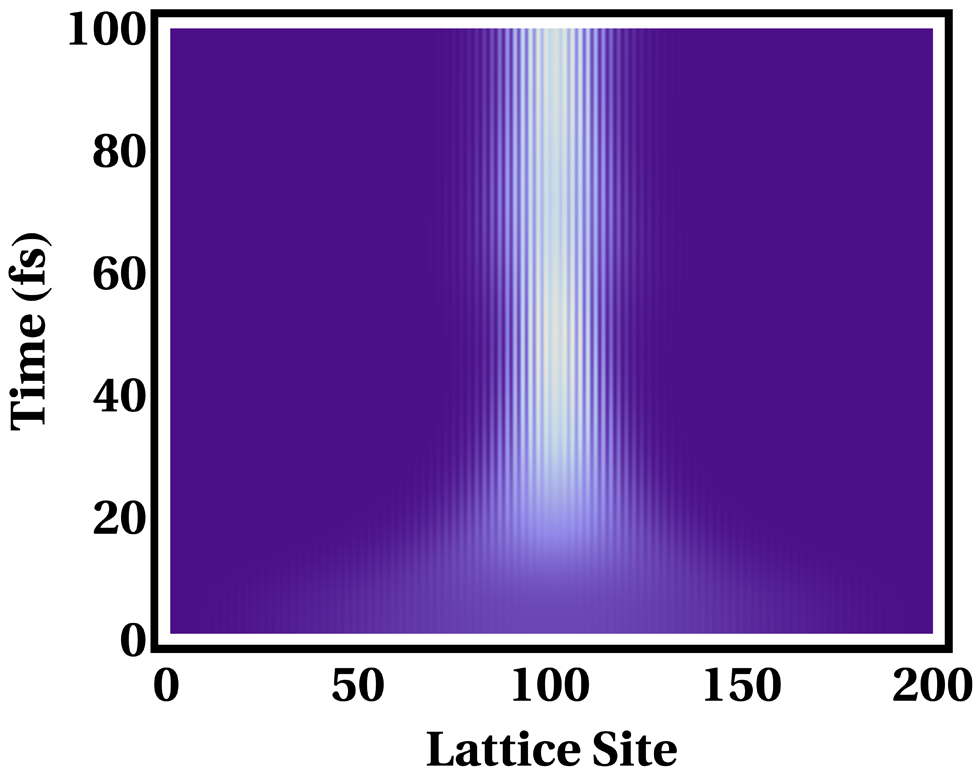
\includegraphics[scale=1]{./figures/Exciton_Figure_6.png}
    \caption{$\Gamma_u$能级电子在聚合物链晶格上出现几率的含时演化}
    \label{fig:wavefun}
\end{figure}

\section{3.2
外界光强对激子局域的影响}\label{ux5916ux754cux5149ux5f3aux5bf9ux6fc0ux5b50ux5c40ux57dfux7684ux5f71ux54cd}

为澄清外界激发光的光强当共轭聚合物分子中激子局域的影响,结合实验结果,我们采用了光强
为\(10\mu J/cm^2\), \(20\mu J/cm^2\), \(30\mu J/cm^2\), \(40\mu J/cm^2\)
的四种不同激光激发有机共轭聚合物分子,展现对不同光强对激子的局域形成的影响。如图
(\ref{fig:pop4}),
随着光强的增加,外界光诱导电子从初始的HOMO跃迁至LUMO后电子占据数的稳定所需的时间逐渐
变短。其中,光强为\(10\mu J/cm^2\)激光诱发一个电子从HOMO跃至LUMO态所需时间为196
飞秒。激光光强为\(20\mu J/cm^2\)时,电子从HOMO跃至LUMO态所需时间为97
飞秒。到外界激光强度
升至\(40\mu J/cm^2\)时,电子跃迁完成的时间减短为为46 飞秒。如
(\ref{fig:l_config})所示,我们分别对比了从\(10\mu J/cm^2\)到\(40\mu J/cm^2\)

\begin{figure}[h!] 
    \centering
    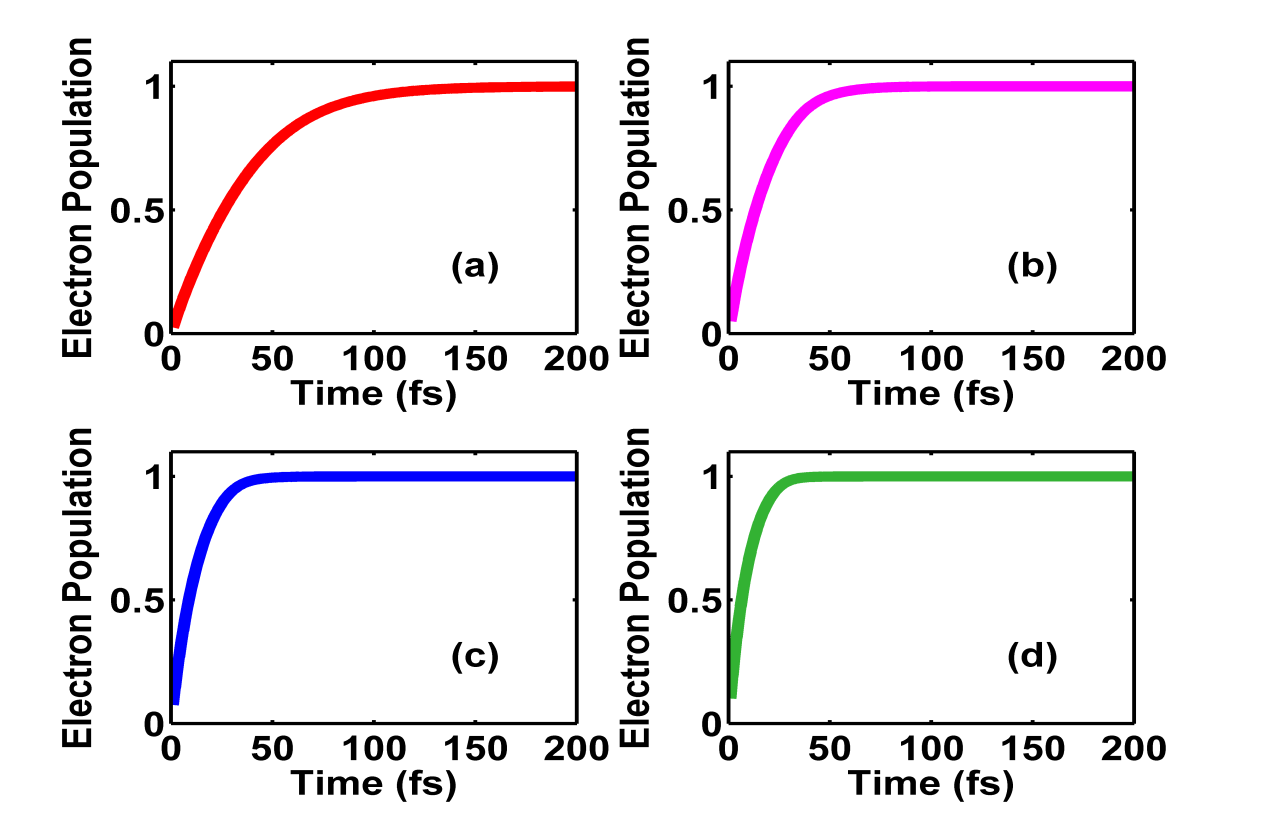
\includegraphics[scale=1]{./figures/Exciton_Figure_11.png}
    \caption{光强为$10\mu J/cm^2$, $20\mu J/cm^2$, $30\mu J/cm^2$, $40\mu J/cm^2$的电子
    占据数}
    \label{fig:pop4}
\end{figure}

\noindent
的4种不同外界光强下,共轭聚合物受激发后的晶格演化过程。由于外界激发光光强的增大,在
激子形成过程中的电子跃迁完成所需时间缩短。由于共轭聚合物分子中电子
-晶格相互作用,相应的晶格位形和电子态的演化也逐渐加速。在外界激发光光强为\(10\mu J/cm^2\)时,晶格位形被稳定的局域所需时间为200
飞秒。当外界激发光光强开始增强,诱发晶格局域畸变的时间也开始缩短。当外界光强增至
\(40\mu J/cm^2\)后,晶格位形被局域畸变的时间缩短至40
飞秒。由于电子晶格相互作用,晶格的局域畸变和新的电子占据数自然地将诱发电子状态的变化。
当聚合物受到外界光激发,作为构成激子状态的电子空穴对中的电子态,由于电子占据数变化显
著如图(\ref{fig:pop}),也自然发生变化,图 (\ref{fig:wavefun})
正是描述了上的电子共轭聚合物分子链上的含时分布过程。与晶格位形演化一致,当外界激发光
光强开始增强,局域激子中电子的时间也开始缩短。当外界光强增至\(40\mu J/cm^2\)后,激子中电子局域的时
间缩短至40
飞秒。可见,外界激发光的强度直接决定了电子跃迁和激子局域的所需时间。由此,也自然的产生
了一个新的问题:激子晶格局域和电子态局域的完成是否标志了激子的形成?最近的实验也发现
,激子的形成时间约为 1000飞秒,
可见激子的局域时间要远早于激子的形成时间。那么是什么原因使得激子形成时间要长于激子局
域的时间呢?

\begin{figure}[h!] 
    \centering
    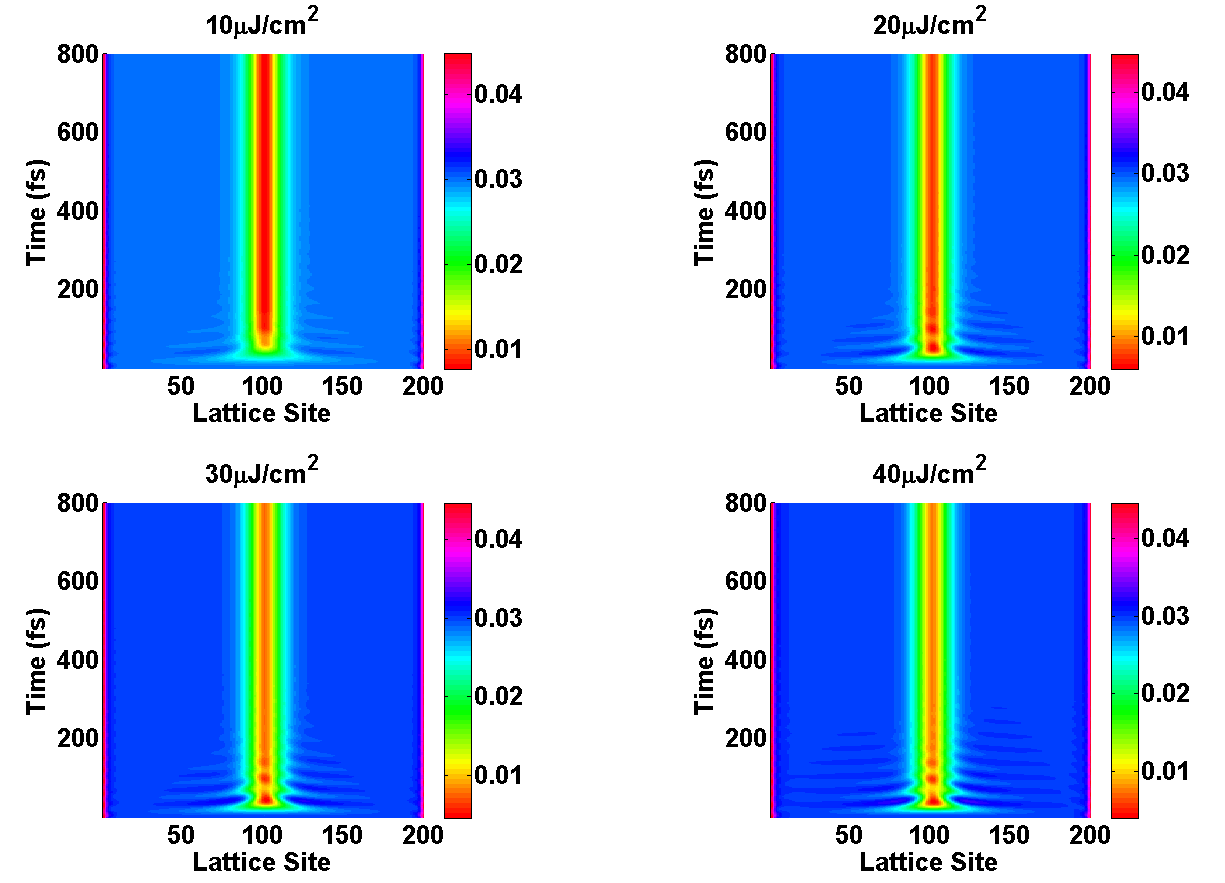
\includegraphics[scale=0.4]{./figures/Exciton_Figure_12.png}
    \caption{光强为$10\mu J/cm^2$, $20\mu J/cm^2$, $30\mu J/cm^2$, $40\mu J/cm^2$的
    晶格位形}
    \label{fig:l_config}
\end{figure}

\section{3.3 激子的弛豫}\label{ux6fc0ux5b50ux7684ux5f1bux8c6b}

为了回答这个问题,我们需关注在更长的时间尺度下激子形成过程中各种能量的变化。当聚合物
分子受到外界激发后,聚合物分子的总能量包括电子的能量、晶格的动能和势能。图(\ref{fig:total_energy})恰恰展现了在光强为\(30\mu J/cm^2\)
的外界激发下在1200飞秒内聚合物分子总能量的演化过程。可以发现,在光激发初始到100飞秒的
时间范围,聚合物分子收到外界光激发后,不仅总能量迅速升至最大值如图
(\ref{fig:total_energy}a) ,而且在100飞秒左右电子的激发跃迁也已完成如图
(\ref{fig:pop}),但此时的总能量并没有处在一个稳定值。聚
合物分子为了让总能量能够到达一个稳定值,进行能量的弛豫成了必要的环节。因此,我们把激
子形成的整个过程分为两部分,激子的电子激发跃迁和激子的弛豫,如图
(\ref{fig:total_energy}a)
所示。完成跃迁激发后聚合物分子则进入了弛豫的过程。从图(\ref{fig:pop4}c)可知在光强为
\(30\mu J/cm^2\)的外界激发下聚合物分子完成激子中的电子跃迁需要64飞秒,而此后则是聚合物
分子的弛豫时间。图(\ref{fig:total_energy}b)描述了弛豫过程中,体系能量经过振荡逐渐达
到一个稳定的值,弛豫过程耗时536飞秒。

\begin{figure}[h!] 
    \centering
    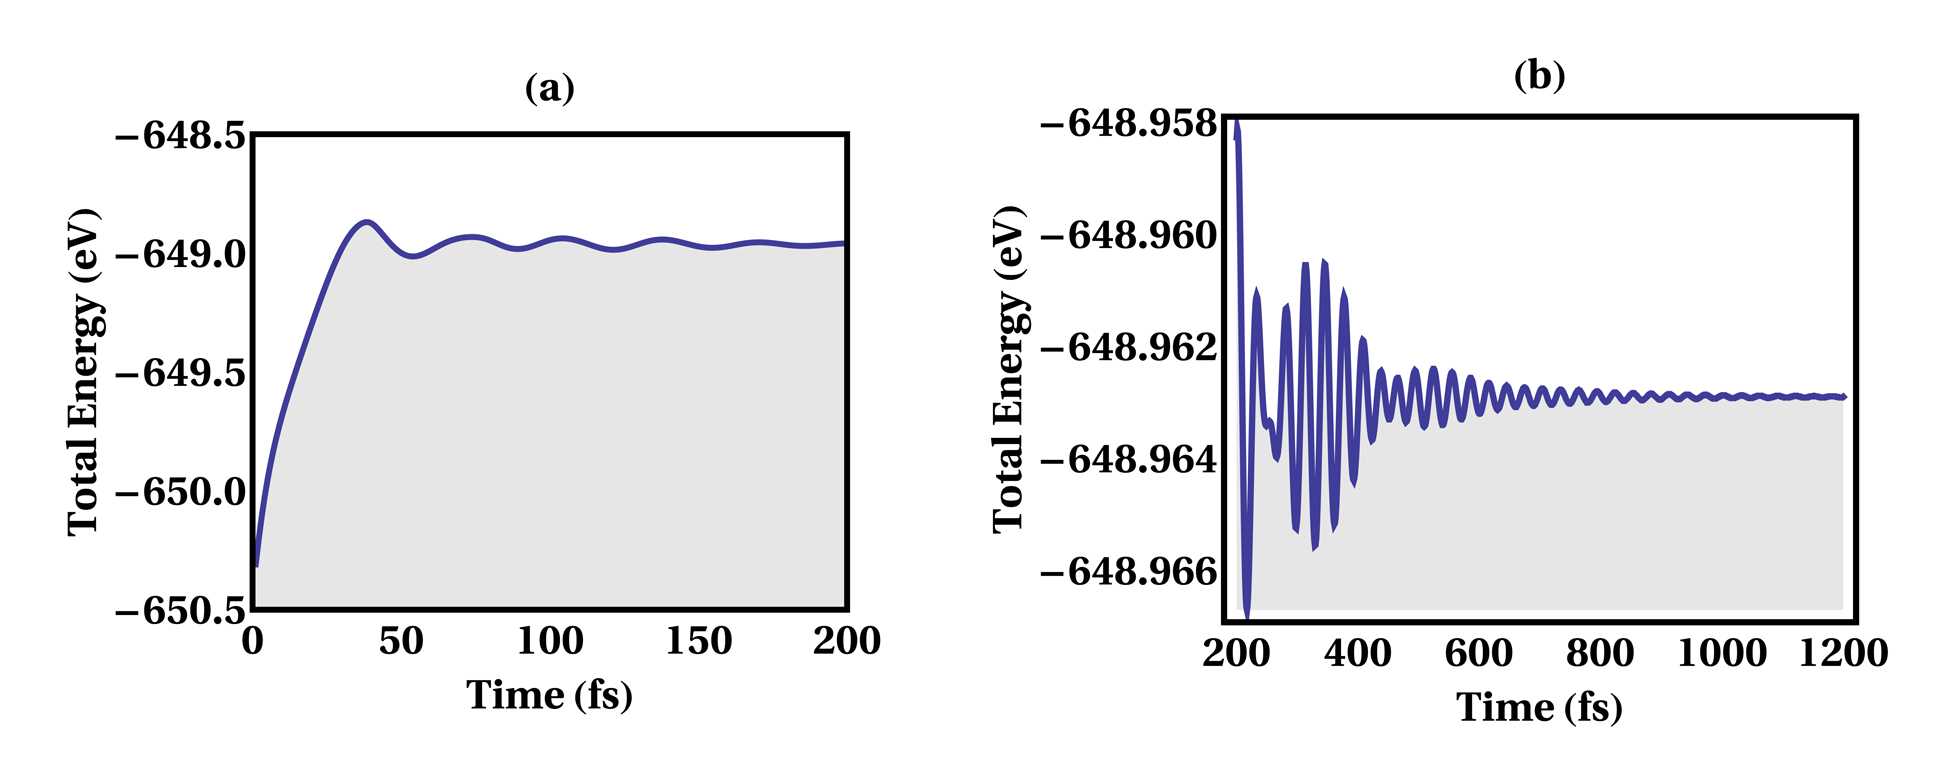
\includegraphics[scale=1]{./figures/Exciton_Figure_7.png}
    \caption{(a)聚合物链的总能量(前200飞秒);(b)聚合物链的总能量(200飞秒到1200飞秒)}
    \label{fig:total_energy}
\end{figure}

\begin{figure}[h!] 
    \centering
    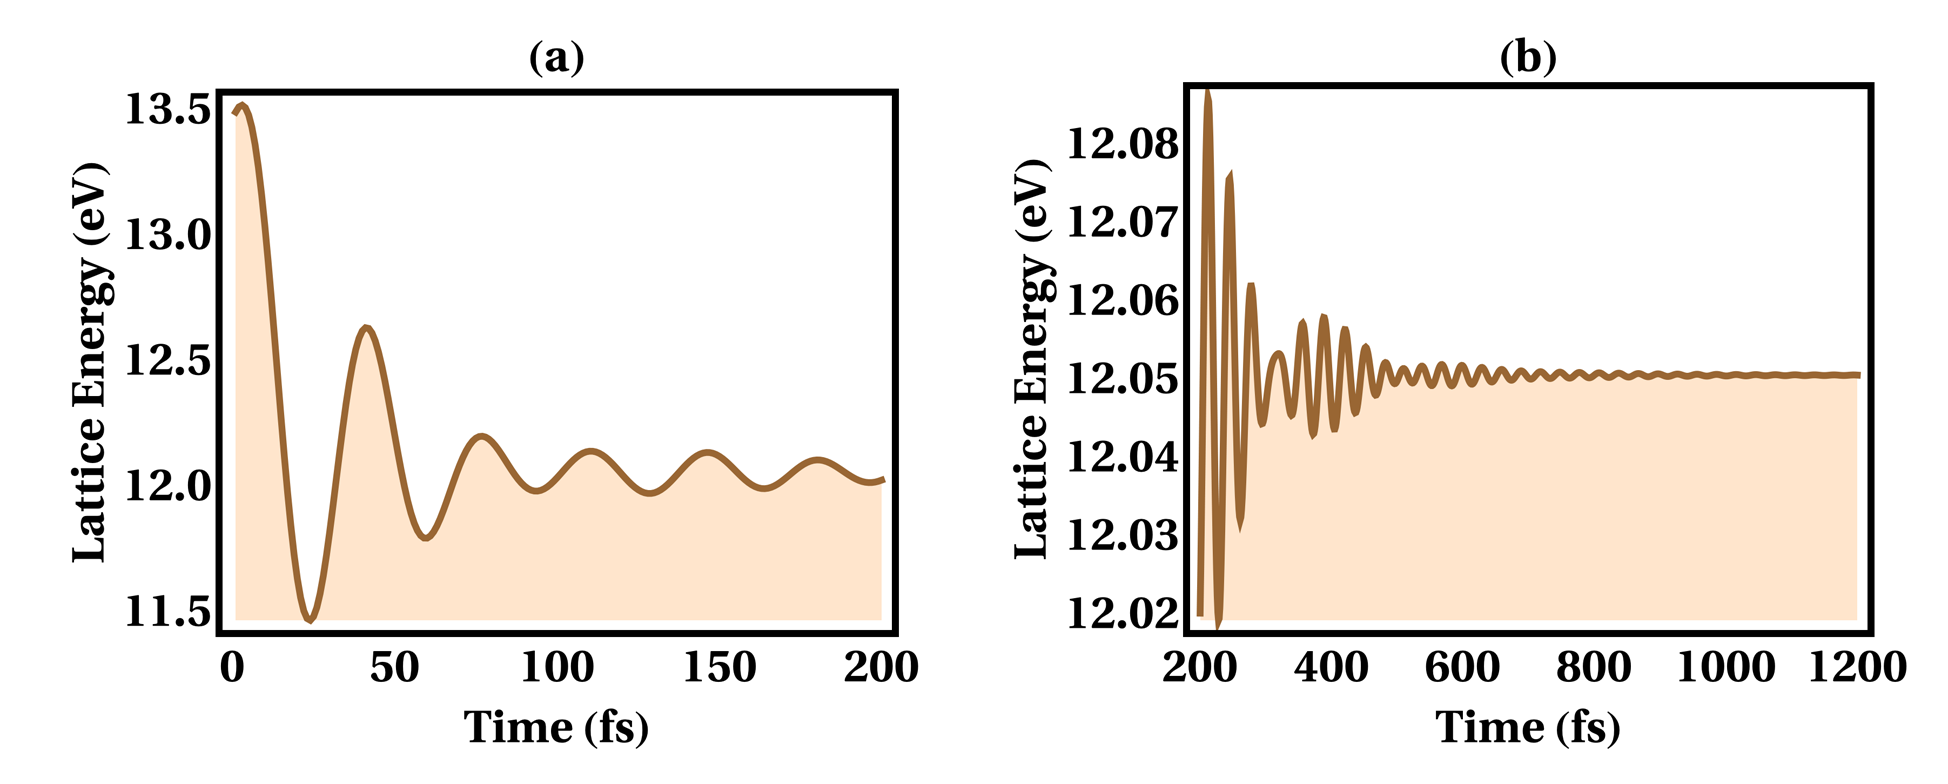
\includegraphics[scale=1]{./figures/Exciton_Figure_8.png}
    \caption{(a)聚合物链中的晶格能量(前200飞秒);(b)聚合物链中的晶格能量(前200飞秒)}
    \label{fig:lattice_energy}
\end{figure}

\begin{figure}[h!] 
    \centering
    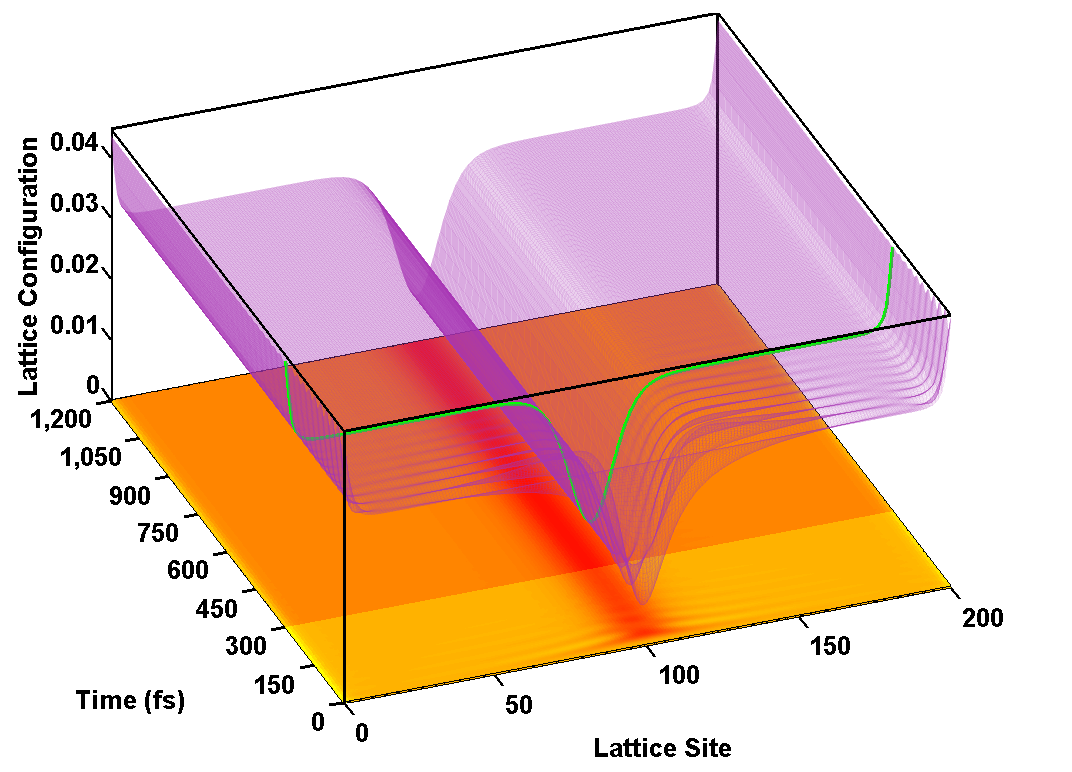
\includegraphics[scale=0.4]{./figures/Exciton_Figure_13.png}
    \caption{聚合物链中晶格位形的演化}
    \label{fig:3dl_config}
\end{figure}

外界光完成激子的电子激发跃迁的同时,恰好也形成了激子的局域,不仅在晶格位形上,还是在
电子状态上。此后,共轭聚合物分子步入了激子形成的弛豫过程。在形成激子的弛豫过程中,聚
合物分子晶格的总能量和电子的能量是如何变化的呢?图(\ref{fig:lattice_energy})刻画了晶
格能量在整个激子形成过程中的演化,其中在激子完成电子跃迁的时间段,即初始的100飞秒内
,晶格动能和势能,如图(\ref{fig:lattice_energy}a)和(\ref{fig:lattice_energy}b),经历
了最大振荡,同时聚合物分子晶格也恰恰出现了局域畸变如图
(\ref{fig:evo_config})
,但分子的晶格的动能和势能并没有处于一个稳定值。在聚合物分子晶格形成局域畸变后,激子
进入了弛豫过程。在考虑存在阻尼的情况下,晶格能量按照约40飞秒的周期缓缓振荡,逐渐稳定
,在800飞秒左右能量处于稳定。与此相对应的是,三维含时的晶格位形演变图
(\ref{fig:3dl_config})清晰的展示,在聚合物分子受激形成激子的晶格局域后,弛豫过程中的
晶格位形整体振荡,在晶格位形演化图的表面留下波痕,但振荡幅度随着时间的演化而逐渐减弱
,直至300飞秒晶格位形开始稳定,并在800飞秒时处于稳定。由于共轭聚合物分子特有的电子晶
格相互作用,晶格的弛豫也诱发了电子弛豫,从图 (\ref{fig:electron_energy})
展示的激子形成过程中电子能量的演化可以看出,在激子完成电子跃迁的100飞秒内,晶格动能
和势能的最大幅度的振荡也诱发了电子能量在此时间段的最激烈的振荡。随后的弛豫过程中,电
子能量也逐渐开始趋于稳定,虽然电子的能量也按照40飞秒的周期缓缓振荡,也在约800飞秒后
收敛。此刻,电子的局域状态也处于稳定的局域状态,如图(\ref{fig:t_wavefun})所示。可见
,当强度为\(30\mu J/cm^2\)的外界光在激发共轭聚合物分子后,在800飞秒左右,聚合物分子的
总能量,晶格的势能,电子的能量,晶格的位形,以及电子的状态,趋于最终稳定,形成激子,
与最近的实验结果相符。

\begin{figure}[h!] 
    \centering
    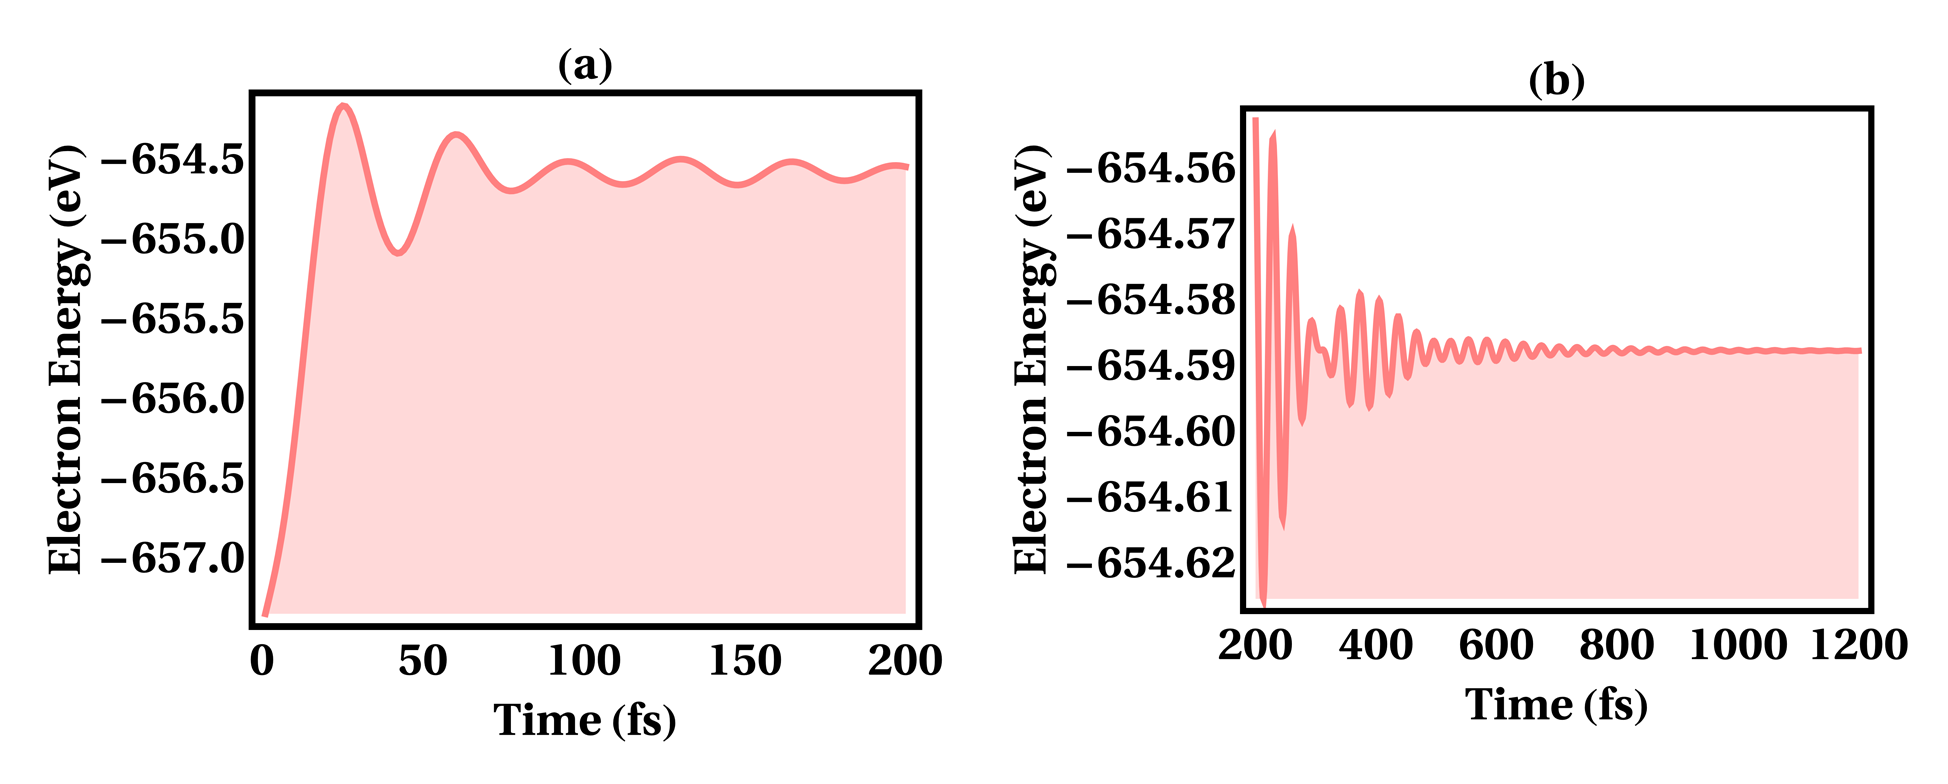
\includegraphics[scale=1]{./figures/Exciton_Figure_9.png}
    \caption{共轭聚合物链中电子能量的演化}
    \label{fig:electron_energy}
\end{figure}

\begin{figure}[h!] 
    \centering
    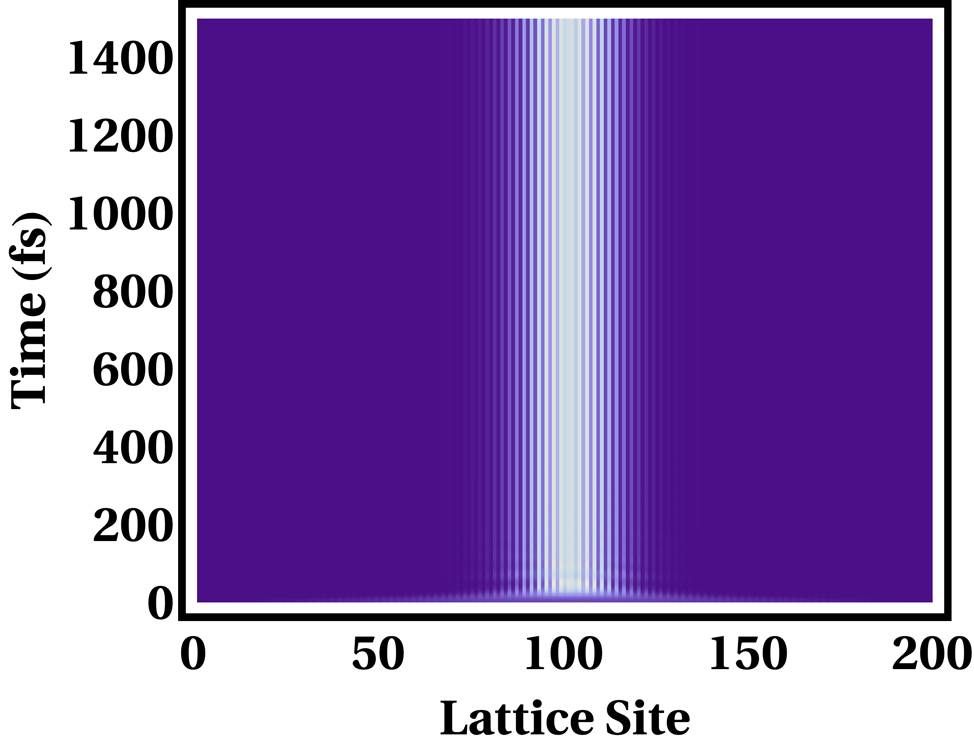
\includegraphics[scale=1]{./figures/Exciton_Figure_10.png}
    \caption{HOMO能级电子在聚合物链晶格上出现几率的含时演化}
    \label{fig:t_wavefun}
\end{figure}

\clearpage

\pagestyle{fancy}

\chapter{半导体聚合物中的载流子输运}\label{ux534aux5bfcux4f53ux805aux5408ux7269ux4e2dux7684ux8f7dux6d41ux5b50ux8f93ux8fd0}

\lhead{} \chead{第四章\quad 有机半导体聚合物中的载流子输运} \rhead{}

半导体聚合物中载流子的状态是极化子态,其中带正电荷的极化子称为正极化子,而带负电荷的
极化子态称为负极化子。在体异质结太阳能电池中,电子空穴对分离后,电子在受体材料中形成
负极化子。本文即讨论负极化子在电场作用下的运动过程。它的电子结构示意图如图(\ref{fig:npolaron})
所示,HOMO上占据了两个自旋相反的电子,LUMO上占据了一个电子。如果将处于稳定基态的负极
化子置于电场环境中,负极化子将会在电场的
作用下发生移动。我们分别研究了基态负极化子和受激的负极化子在电场中的运动。

\begin{figure}[h!] 
    \centering
    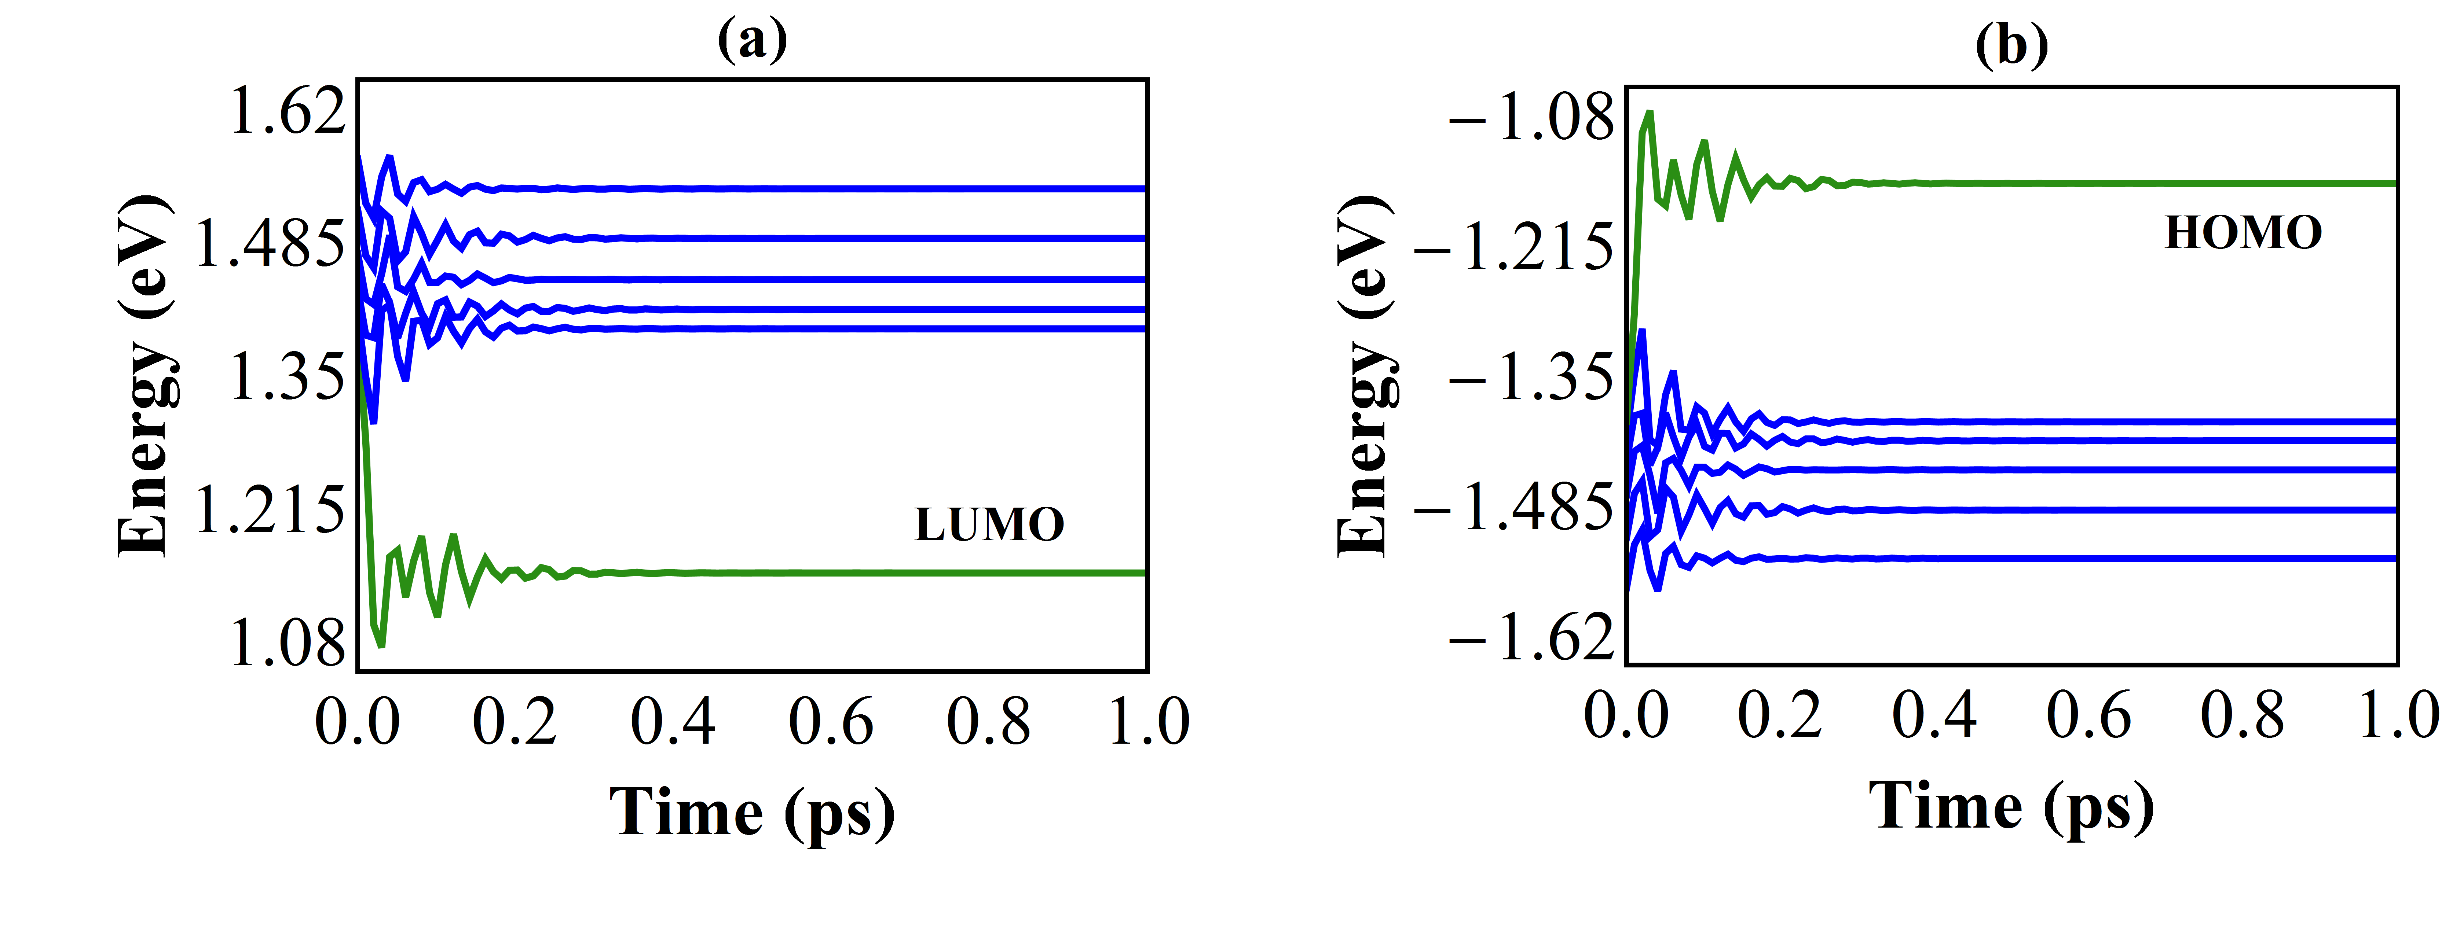
\includegraphics[scale=0.5]{./figures/energy_change.png}
    \caption{靠近HOMO与LUMO能级的含时演化}
    \label{fig:energy_change}
\end{figure}

\section{4.1
基态极化子的输运性质}\label{ux57faux6001ux6781ux5316ux5b50ux7684ux8f93ux8fd0ux6027ux8d28}

为了描述的方便,我们仍然用200个聚合物单体组成的一维聚合物链进行模拟。在聚合物太阳能
电池中,一个受光激发的激子在给体与受体的界面处被拆分成了带电荷的载流子。在这个过程中
,图(\ref{fig:energy_change})给出了靠近HOMO与LUMO能级(蓝色)及其本身(绿色)的含时演化
过程。我们可以看到,HOMO与LUMO的能级分别离开了它原本的状态,而在能隙中间表现为局域。
为了简单表示这个过程,我们用图(\ref{fig:polaron})来表示这个过程。为了表述的方便,我
们重新命名了原本的LUMO能级为\(\Gamma_u\),HOMO能级为\(\Gamma_d\)。

\begin{figure}[h!]
    \centering
    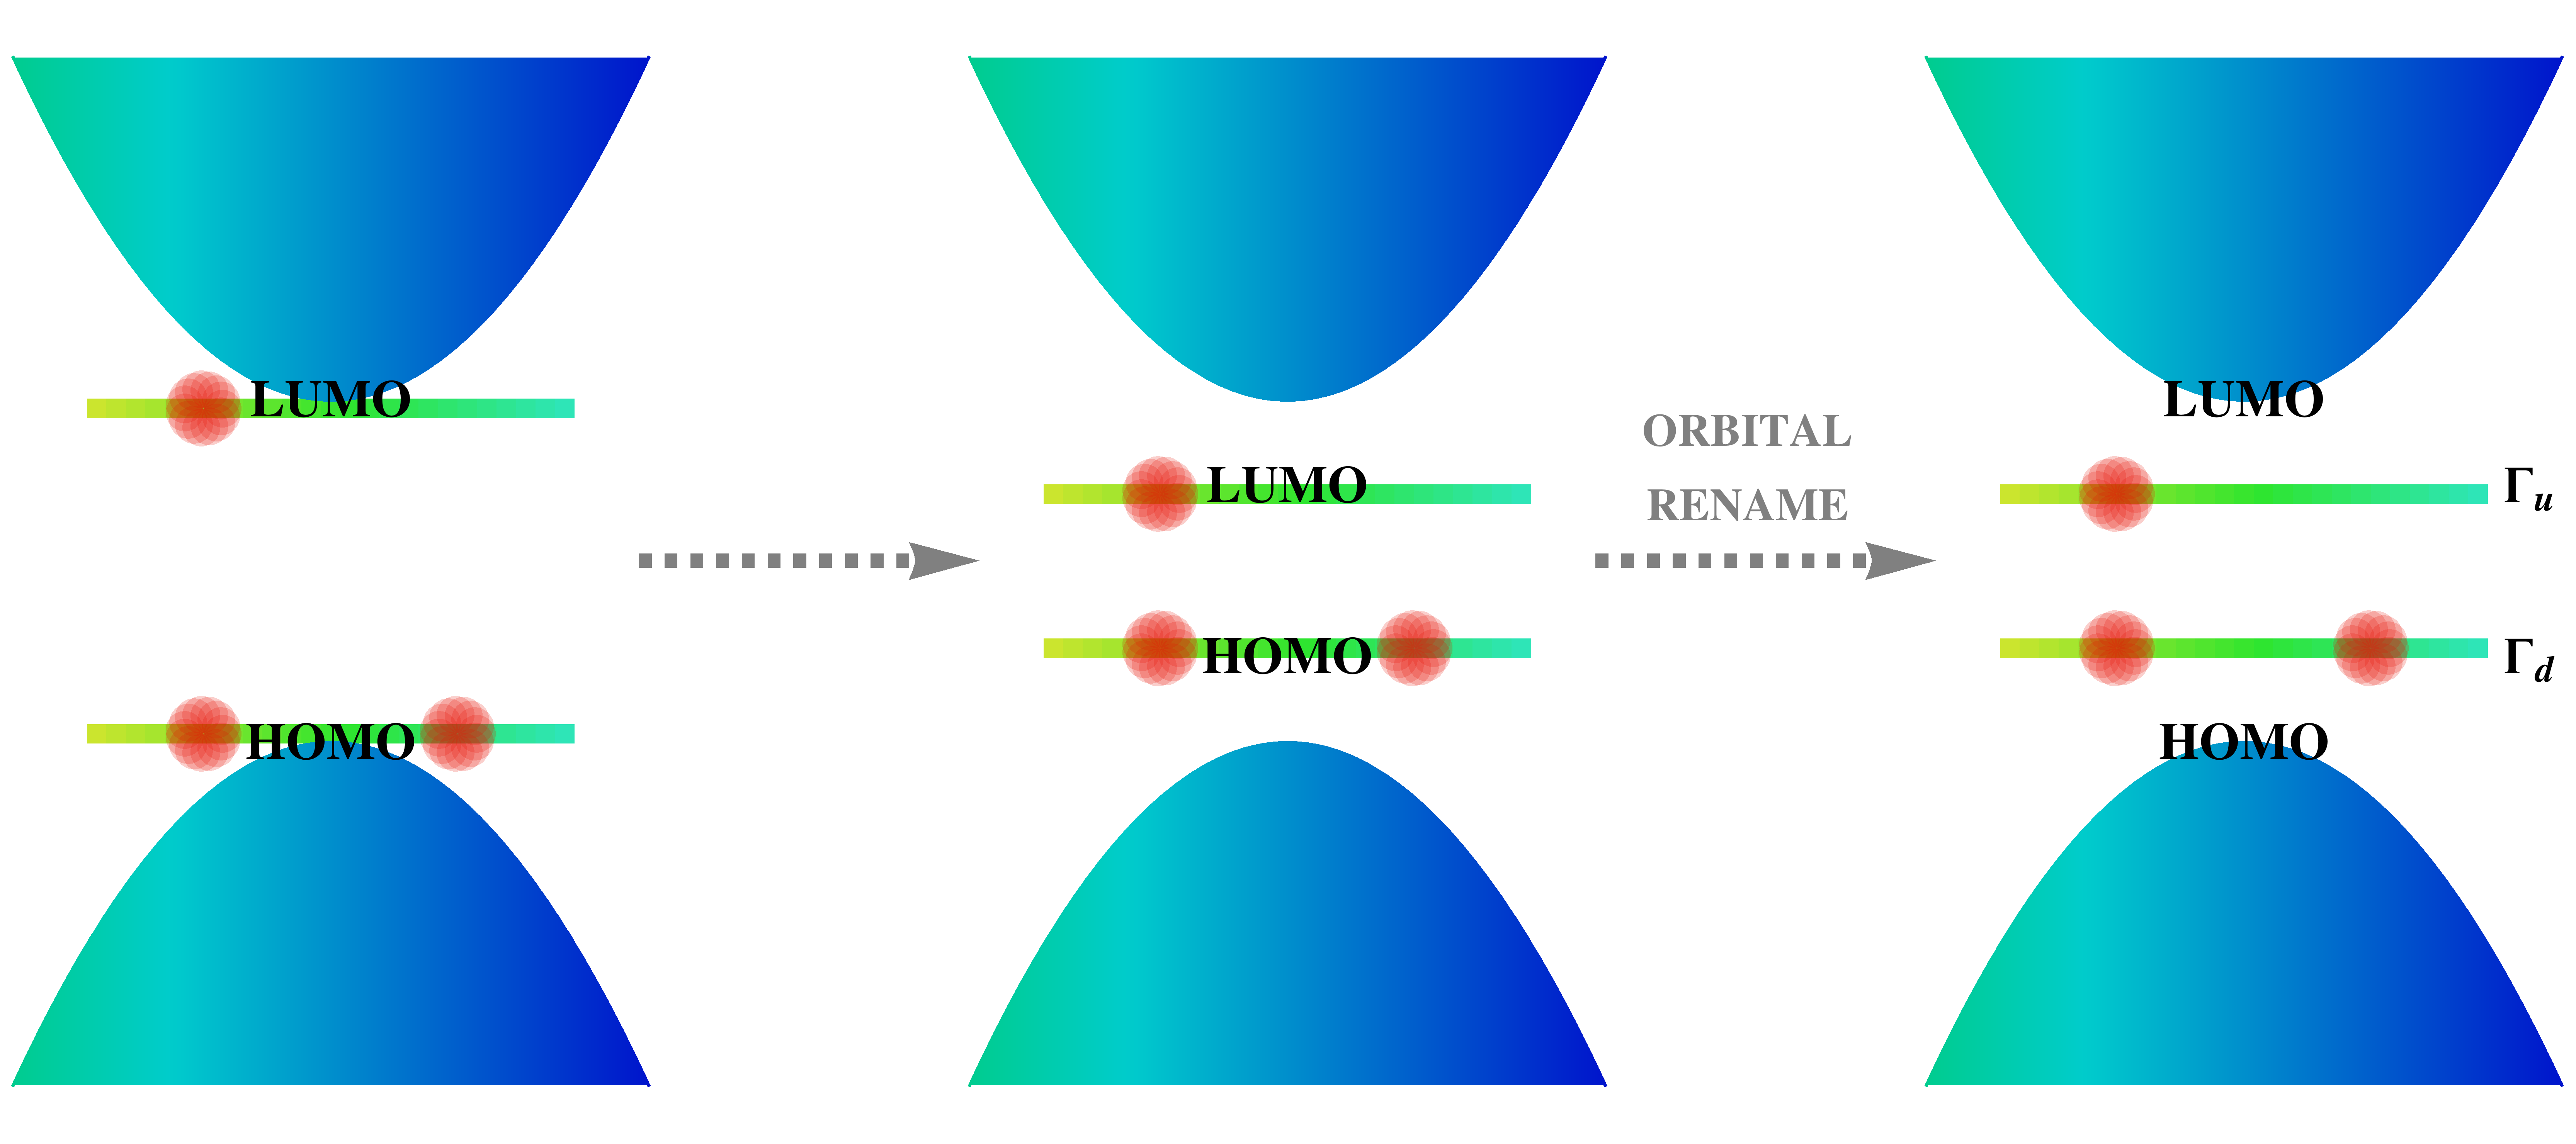
\includegraphics[scale=0.5]{./figures/polaron.png}
    \caption{在能带结构中,电子注入聚合物引起的能带变化并形成的负极化子}
    \label{fig:polaron}
\end{figure}

\begin{figure}[h!]
    \centering
    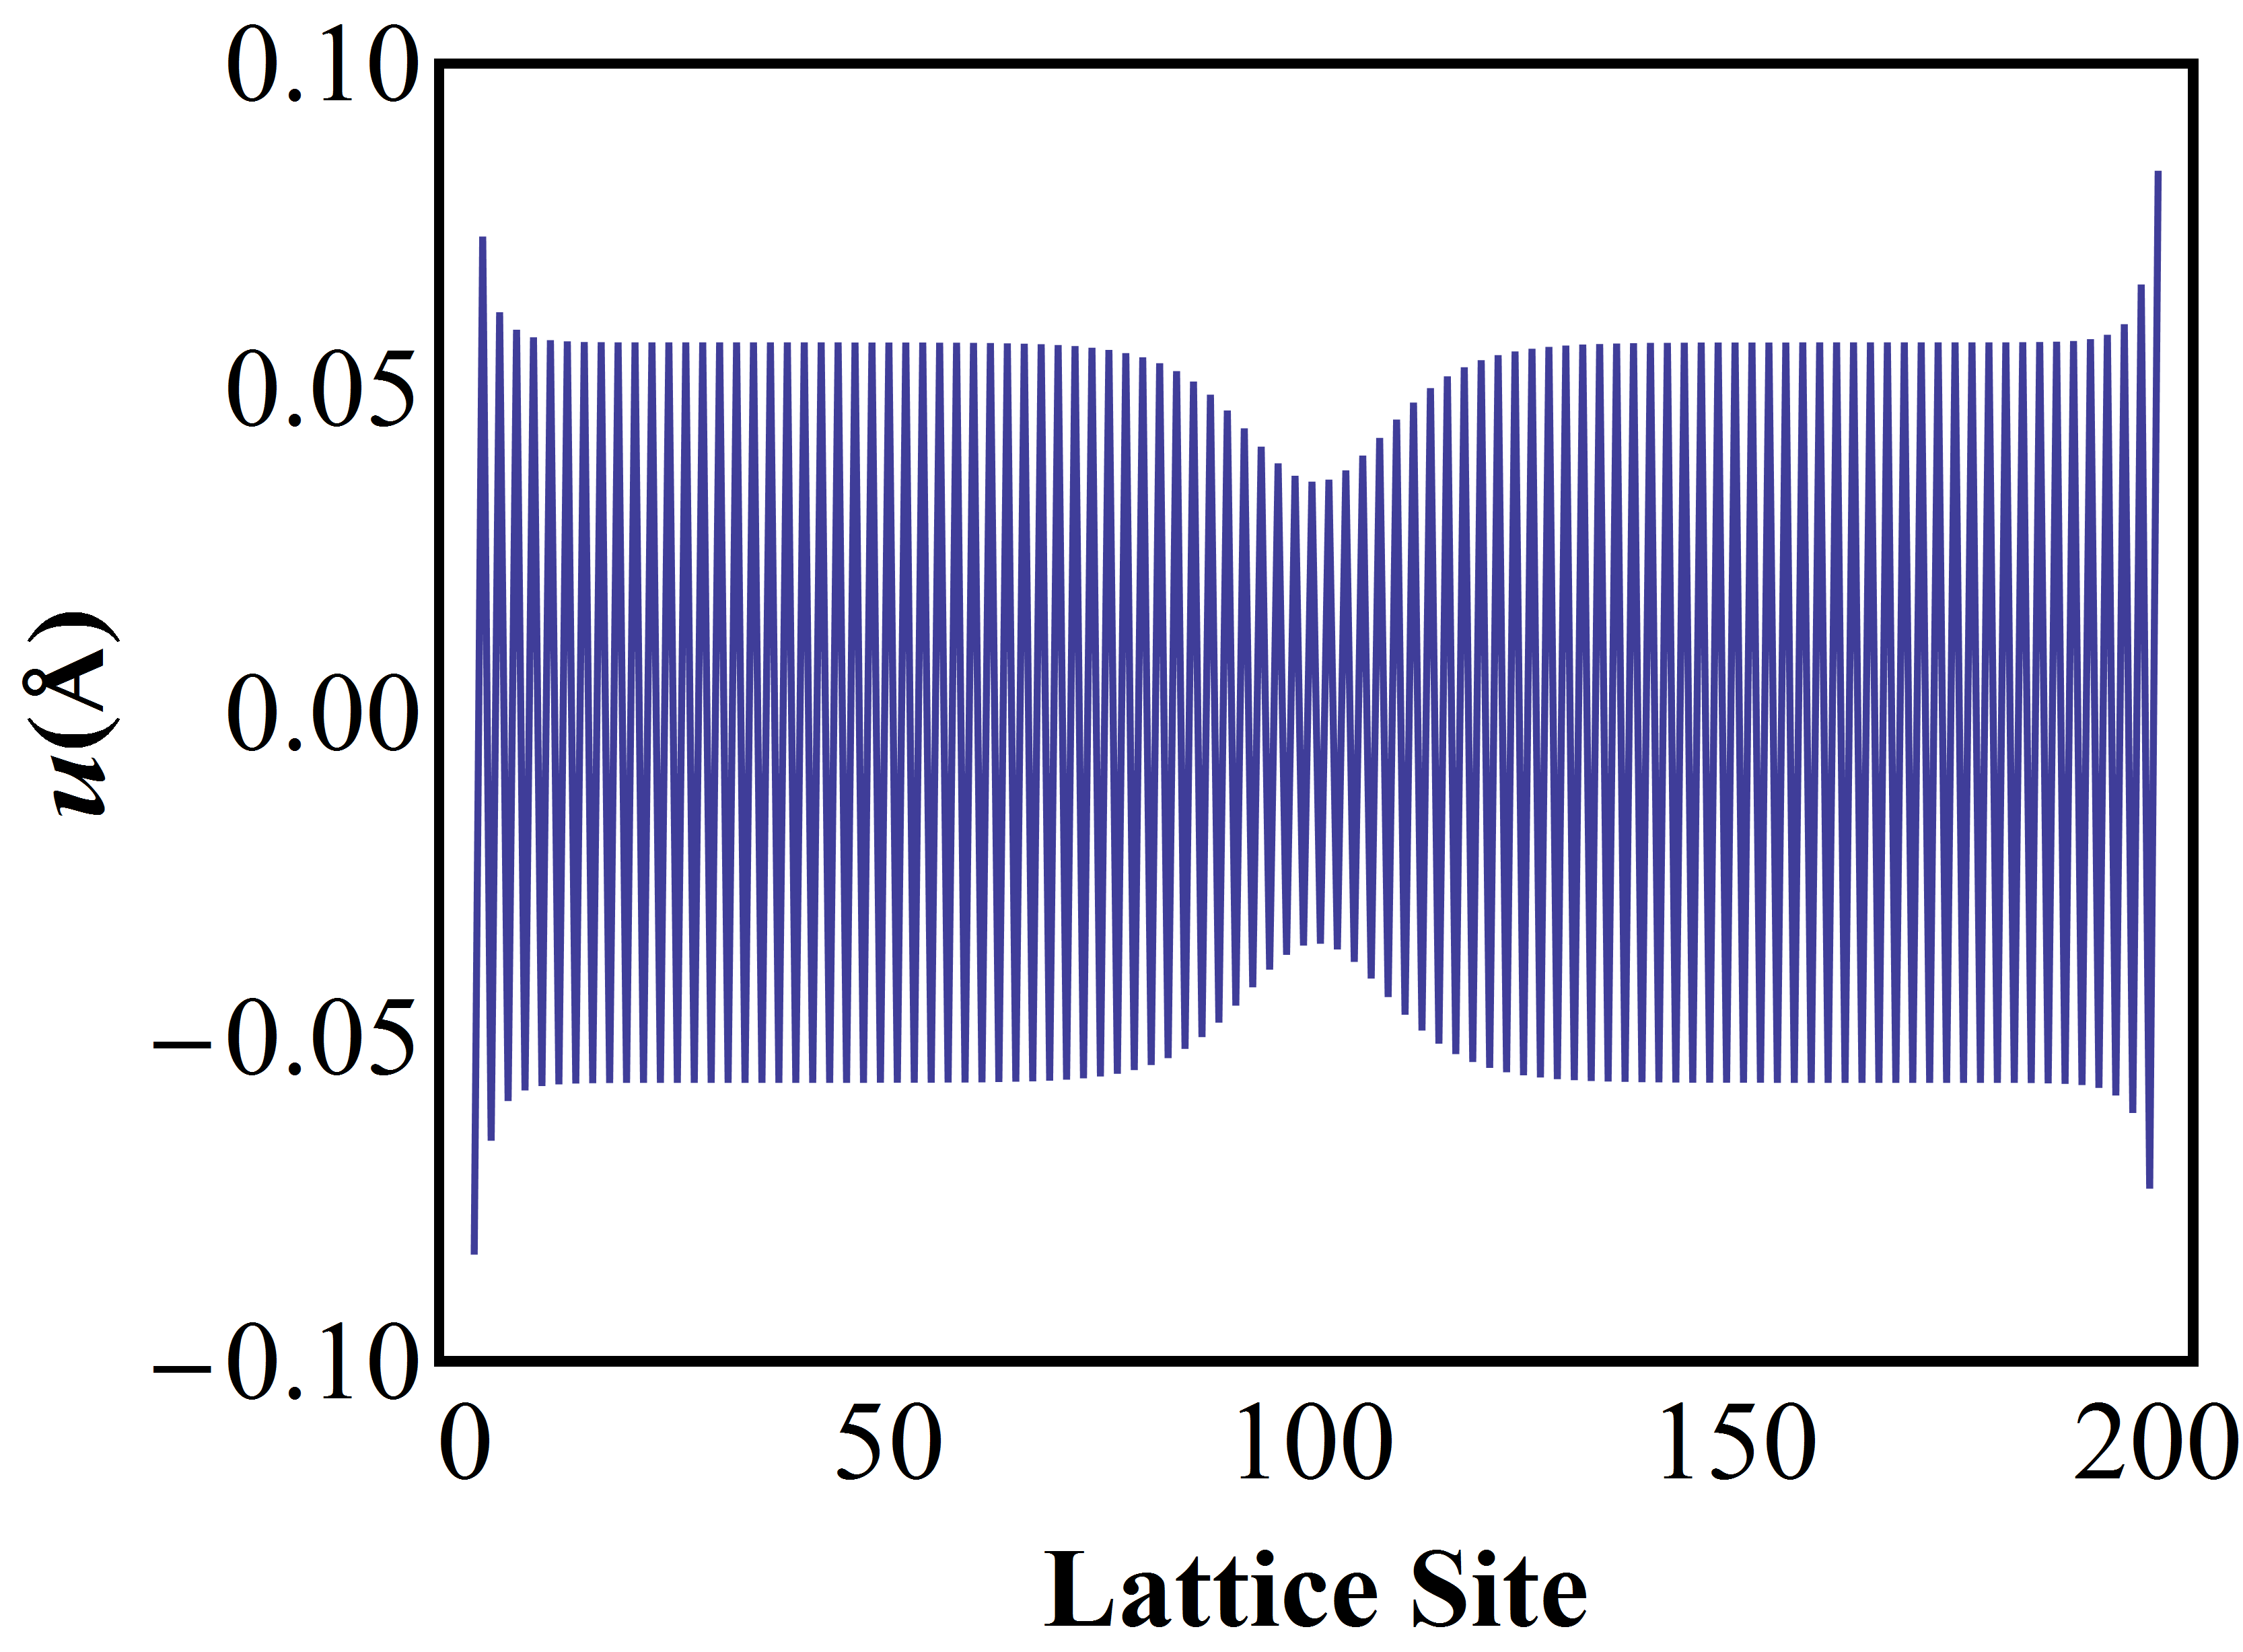
\includegraphics[scale=0.5]{./figures/polaron_lattice.png}
    \caption{极化子引起的晶格畸变}
    \label{fig:polaron_lattice}
\end{figure}

\begin{figure}[h!]
    \centering
    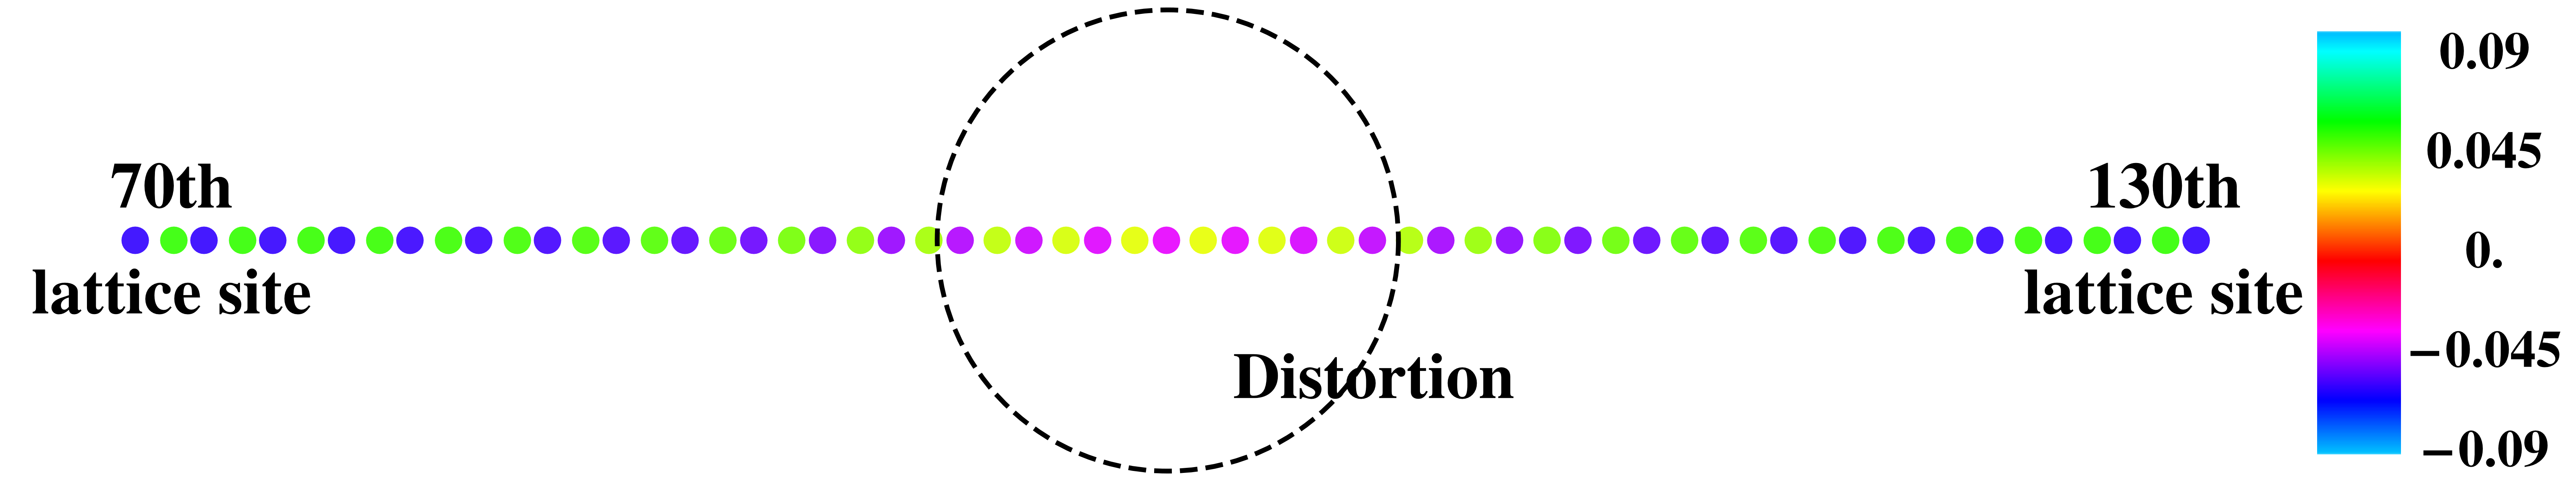
\includegraphics[scale=0.5]{./figures/chain.png}
    \caption{基态时的负极化子在晶格上形成的畸变}
    \label{fig:chain}
\end{figure}

因为在聚合物链中输运的载流子是一个极化子,我们考虑其因为电子-声子相互作用引起的晶格
位型的变化:极化子的存在会让晶格位型发生畸变,如图(\ref{fig:polaron_lattice})。这里
,我们用晶格单体位移的绝对值\(u\)来描述晶格位型。其中靠近链中间的大部分的值都大于
\(-0.05\)\AA,但略小于\(0.05\)\AA。这部分值是由负极化子引起的畸变导致的。如果我们把晶格
的位移用颜色来表示来进行聚合物链畸变的可视化。如图(\ref{fig:chain})描述的是晶格链中
位于第70个单体到130个单体的一段子链。畸变的这部分可以很明显地从颜色的不同模式中发现
,其位于第100个晶格位置,即聚合物链的中间部分。

在外界电场的作用下,一个负极化子在聚合物链上沿着电场方向相反的方向运动。为了描述这种
运动,一个处于基态的极化子在电场下的运动被研究了。如图
(\ref{fig:epolaron})
所示,电场开始作用于极化子上的初始时刻,令极化子处于第50个格点的位置上。在电场作用下
,极化子开始朝大于50个格点的方向运动,直到600飞秒时,极化子已经运动到大约150个格点位置
。在整个运动的过程中,极化子的运动位移
与运动时间的关系基本保持线性关系。也就是说,极化子在电场中的运动几乎是表现为线性的匀
速的运动。除了让极化子发生运动,电场是否会影响极化子的能级结构的特点?能级结构可以直
接从电子在能级上的占据数来表征。图 (\ref{fig:pop41})
是上局域能级的电子占据数随时间的变化关系。我们在0飞秒时刻开始加入电场的作用,从图
(\ref{fig:pop41})
可以看到,电子的占据数在初始时刻,代表了极化子正处于基态。随着电场的作用,该能级
上的电子占据数始终为0,没有发生变化,这代表了在电场的作用下,极化子在每一个时刻都仍
然处于基态。总之,电场作用下的基态极化子会在晶格链上发生位移,然而不会改变极化子的能
级结构,原本处于基态的极化子始终处于基态。

\begin{figure}[h!]
    \centering
    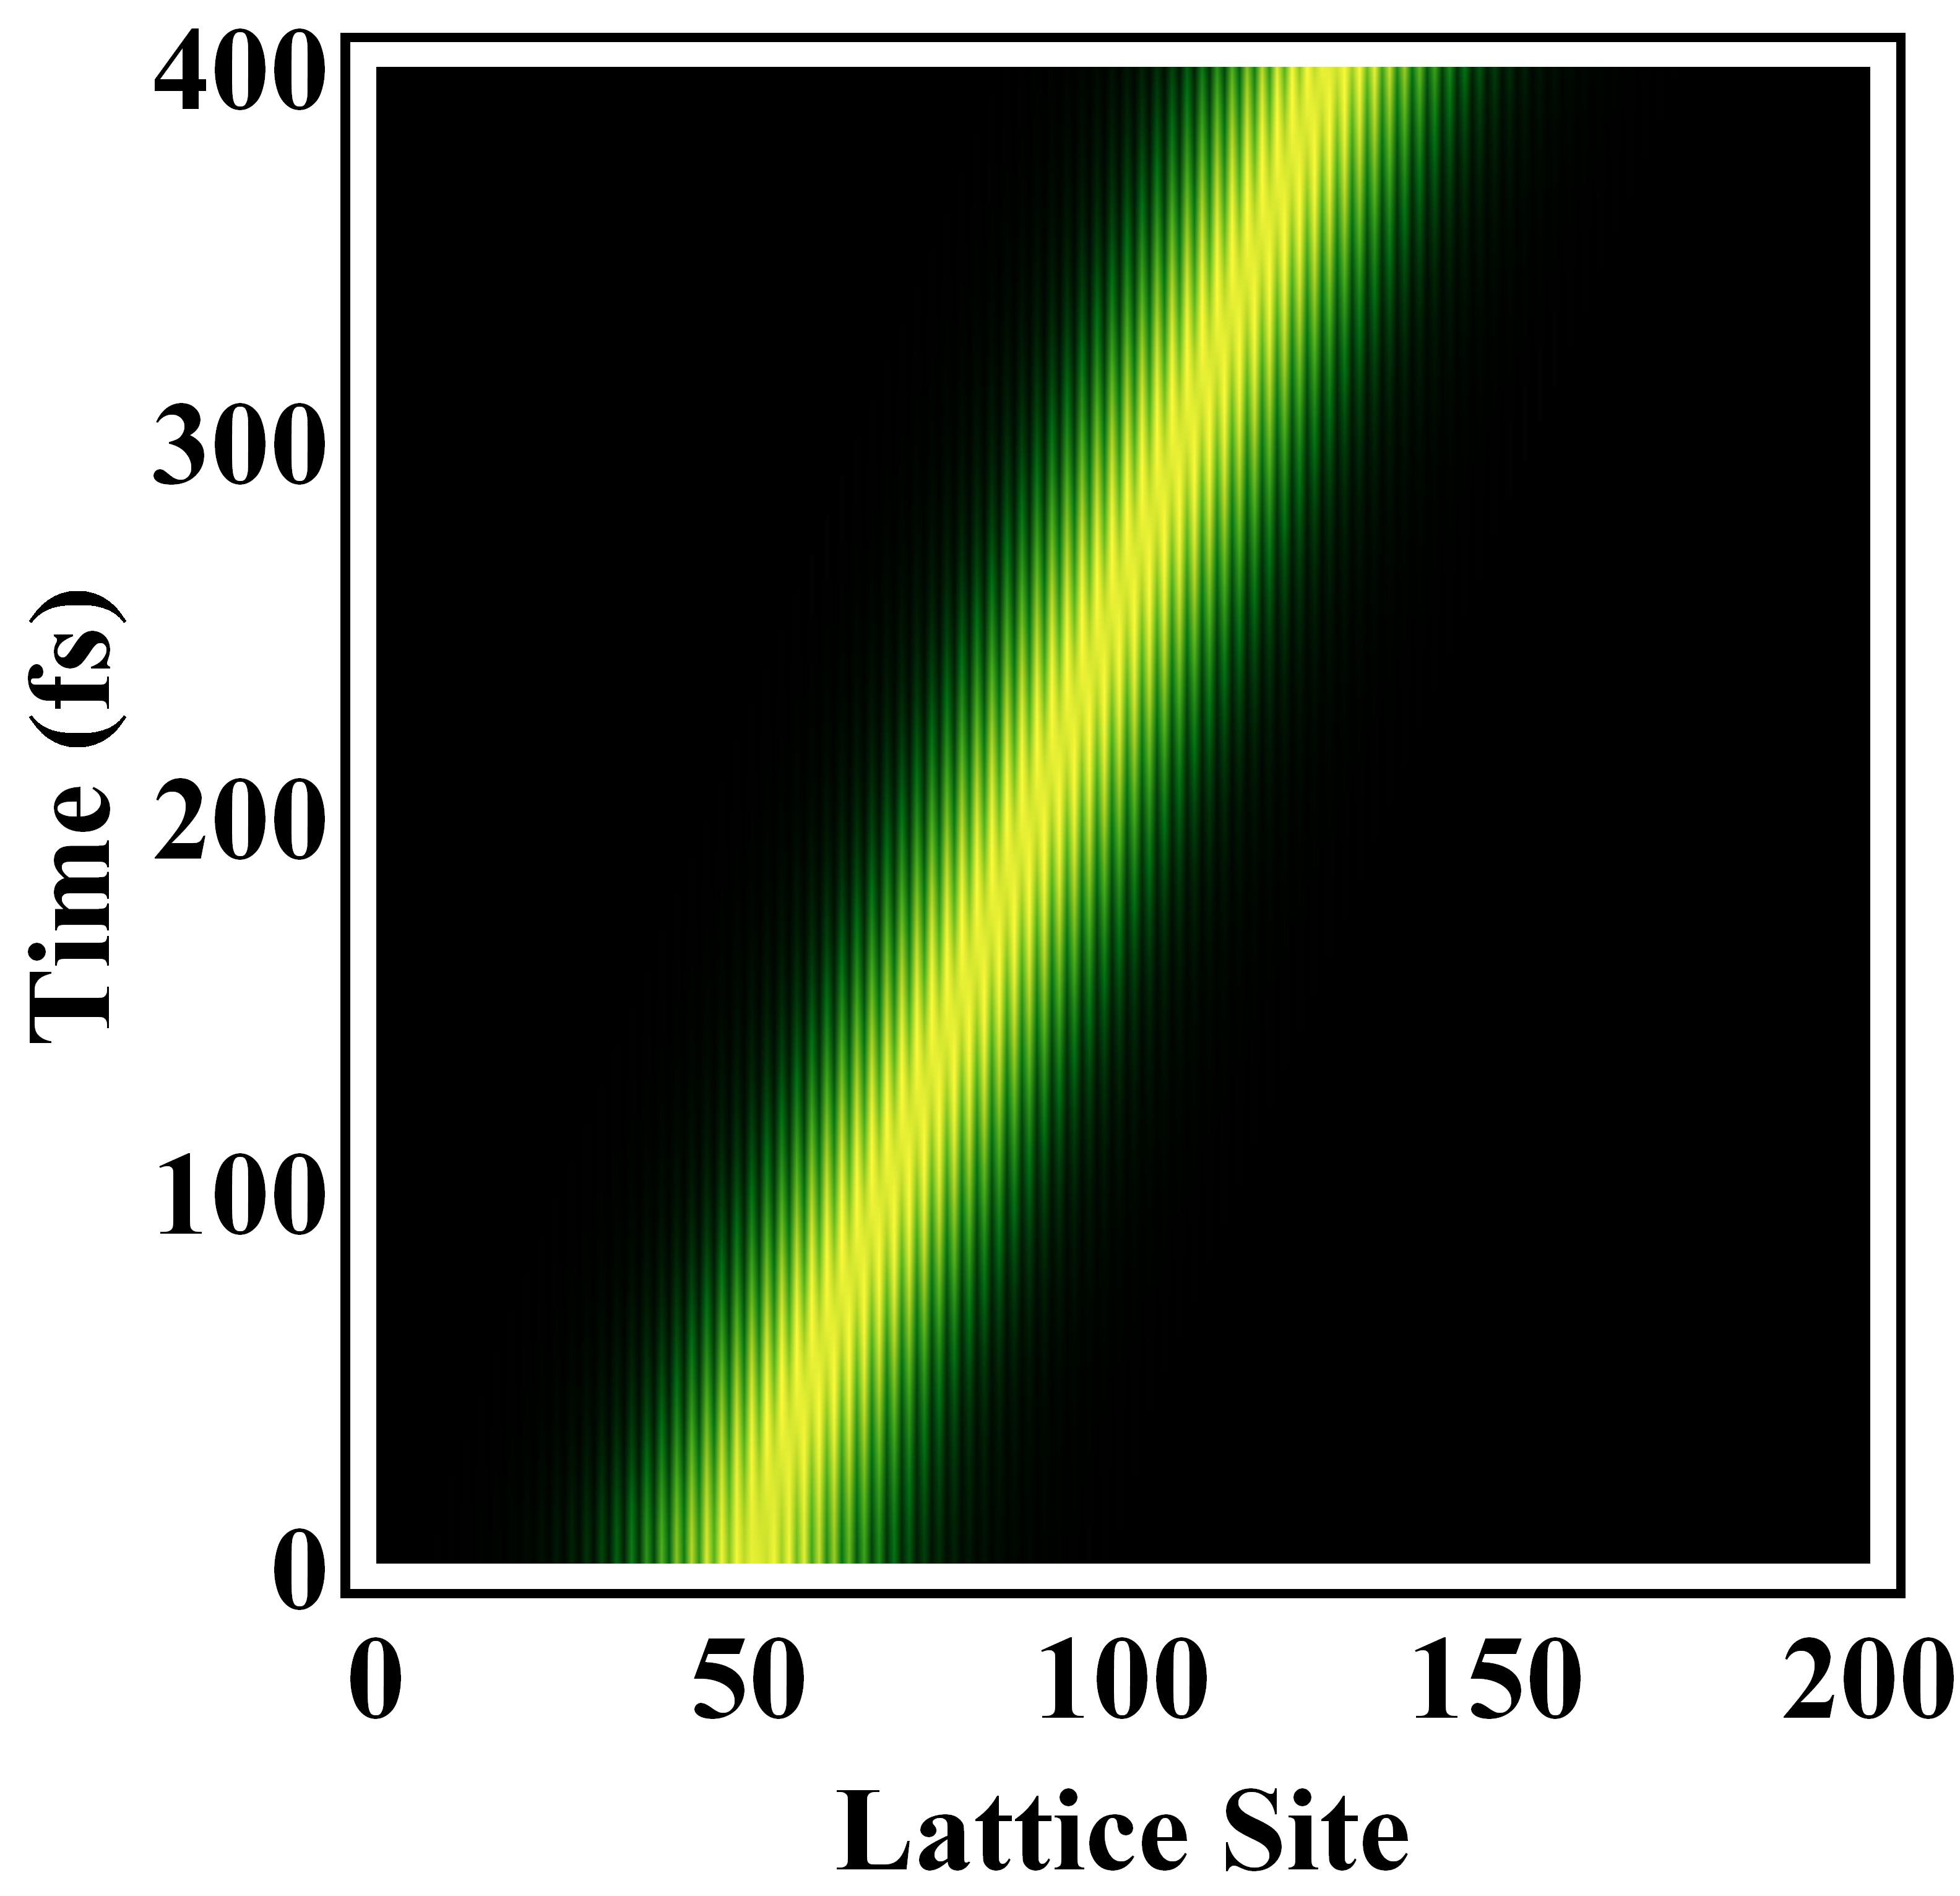
\includegraphics[scale=0.5]{./figures/epolaron.png}
    \caption{电场下运动的负极化子}
    \label{fig:epolaron}
\end{figure}

\begin{figure}[h!]
    \centering
    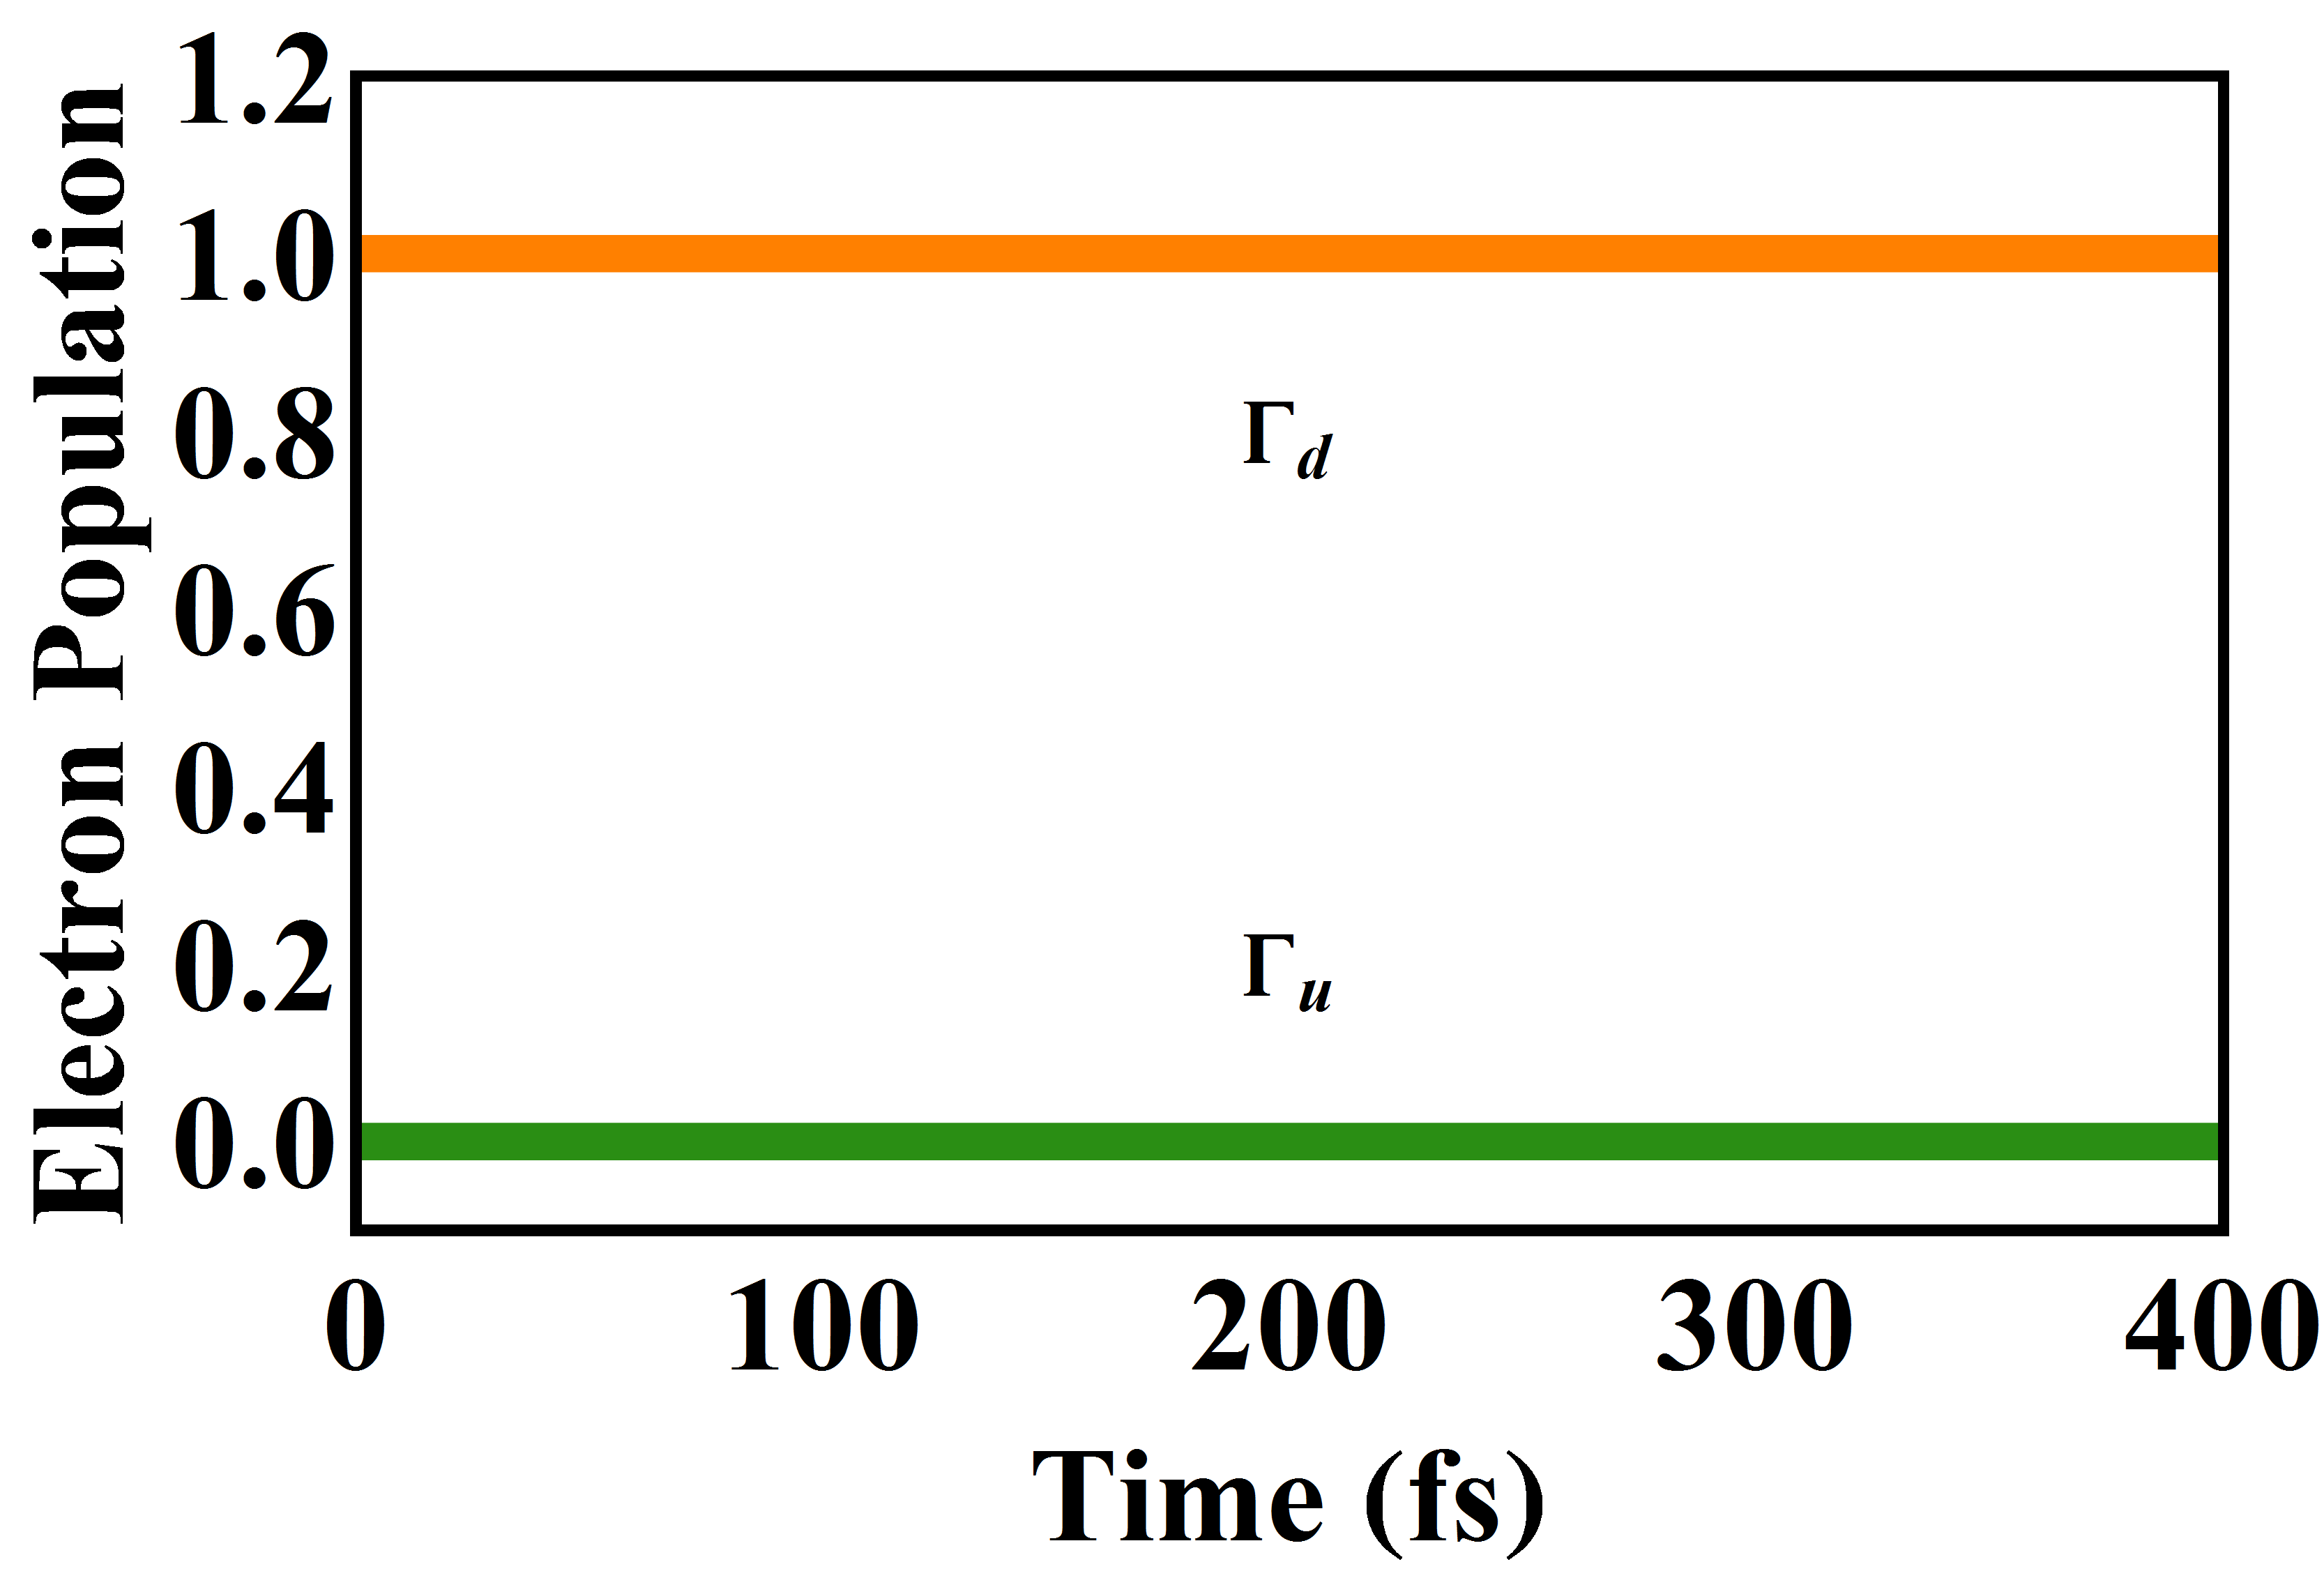
\includegraphics[scale=0.5]{./figures/pop41.png}
    \caption{电子占据数的含时演化}
    \label{fig:pop41}
\end{figure}

但是,在外界的光激发下,极化子将会发生能级结构的改变,形成新的能级结构而处于激发态。
我们研究极化子仅在外界光激发下的运动并展示其能级结构如何随激发的过程而改变。在0飞秒时
刻,我们将20 外界光强开始作用于基态的极化子上。如图
(\ref{fig:polaron_photon})
所示,令极化子在0飞秒时刻处于第50个晶格的位置上。可以看到,随着外界光激发的进行,
在600飞秒内极化子的位移始终没有发生变化。因此,光强对极化子的激发作用并不会使得极化子
发生其在晶格位置上的改变。那么,光激发强度将怎样改变极化子的能级结构?如图
(\ref{fig:pop42})
所示的是上局域能级的电子占据数随时间的变化,在0飞秒时刻,我们将外界光强开始作用于基
态的极化子上,此时电子的占据数为0,在光激发的100飞秒内,上局域能级的电子占据数迅速的趋
向并靠近 0.5
。随着光激发的进行,该能级的电子占据数几乎不再发生变化。可以清晰地看到,将0飞秒时刻与
400飞秒时刻的上局域能级电子占据数进行比较,可以发现该电子占据数从0变化到了
0.5
,这代表了极化子的能级结构发生了改变,极化子脱离基态的状态而形成了激发态。同时,考虑
到上下局域能级的电子占据总数设为1,导致了该激发态的上局域能级占据数和下局域能级的占
据数相同,都为 0.5
。综上所述,在外界光激发作用下,极化子并不会发生在晶格上的位移,对其有意义的是,极化
子的能级结构将发生改变,导致极化子不再处于基态而形成一个新的激发状态。

\begin{figure}[h!]
    \centering
    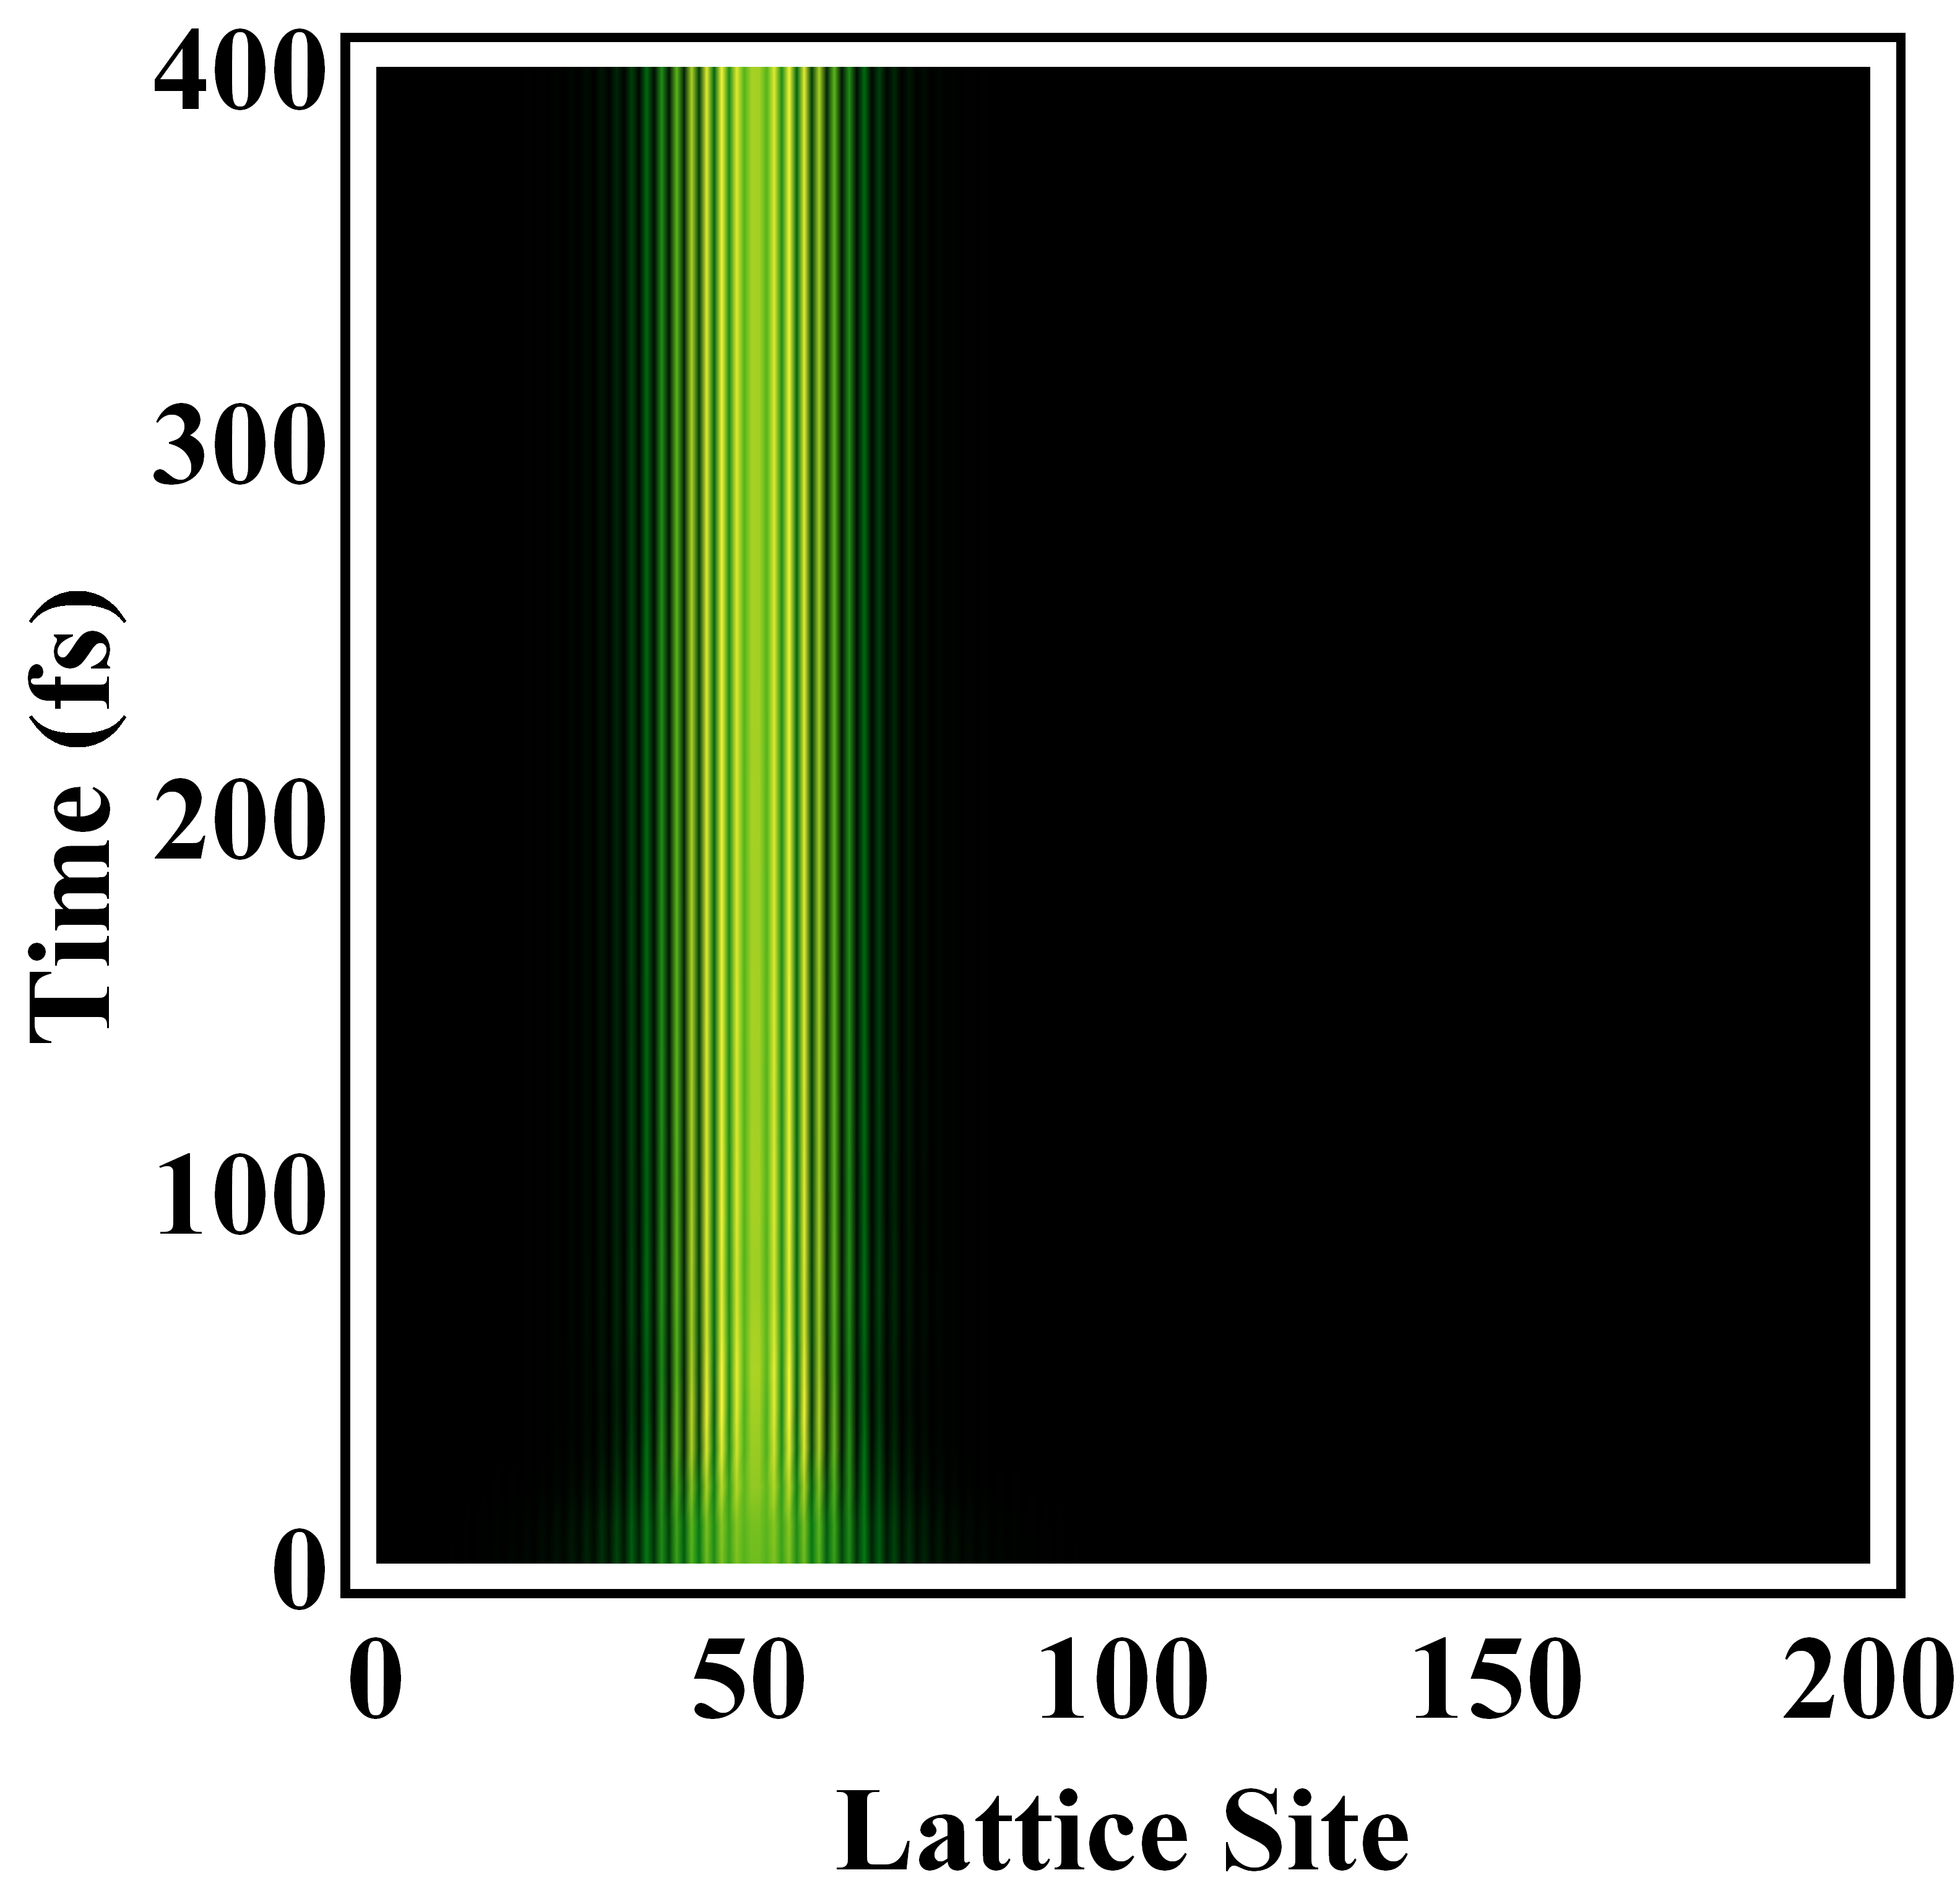
\includegraphics[scale=0.5]{./figures/epolaron_photon.png}
    \caption{光场下运动的负极化子}
    \label{fig:polaron_photon}
\end{figure}

\begin{figure}[h!]
    \centering
    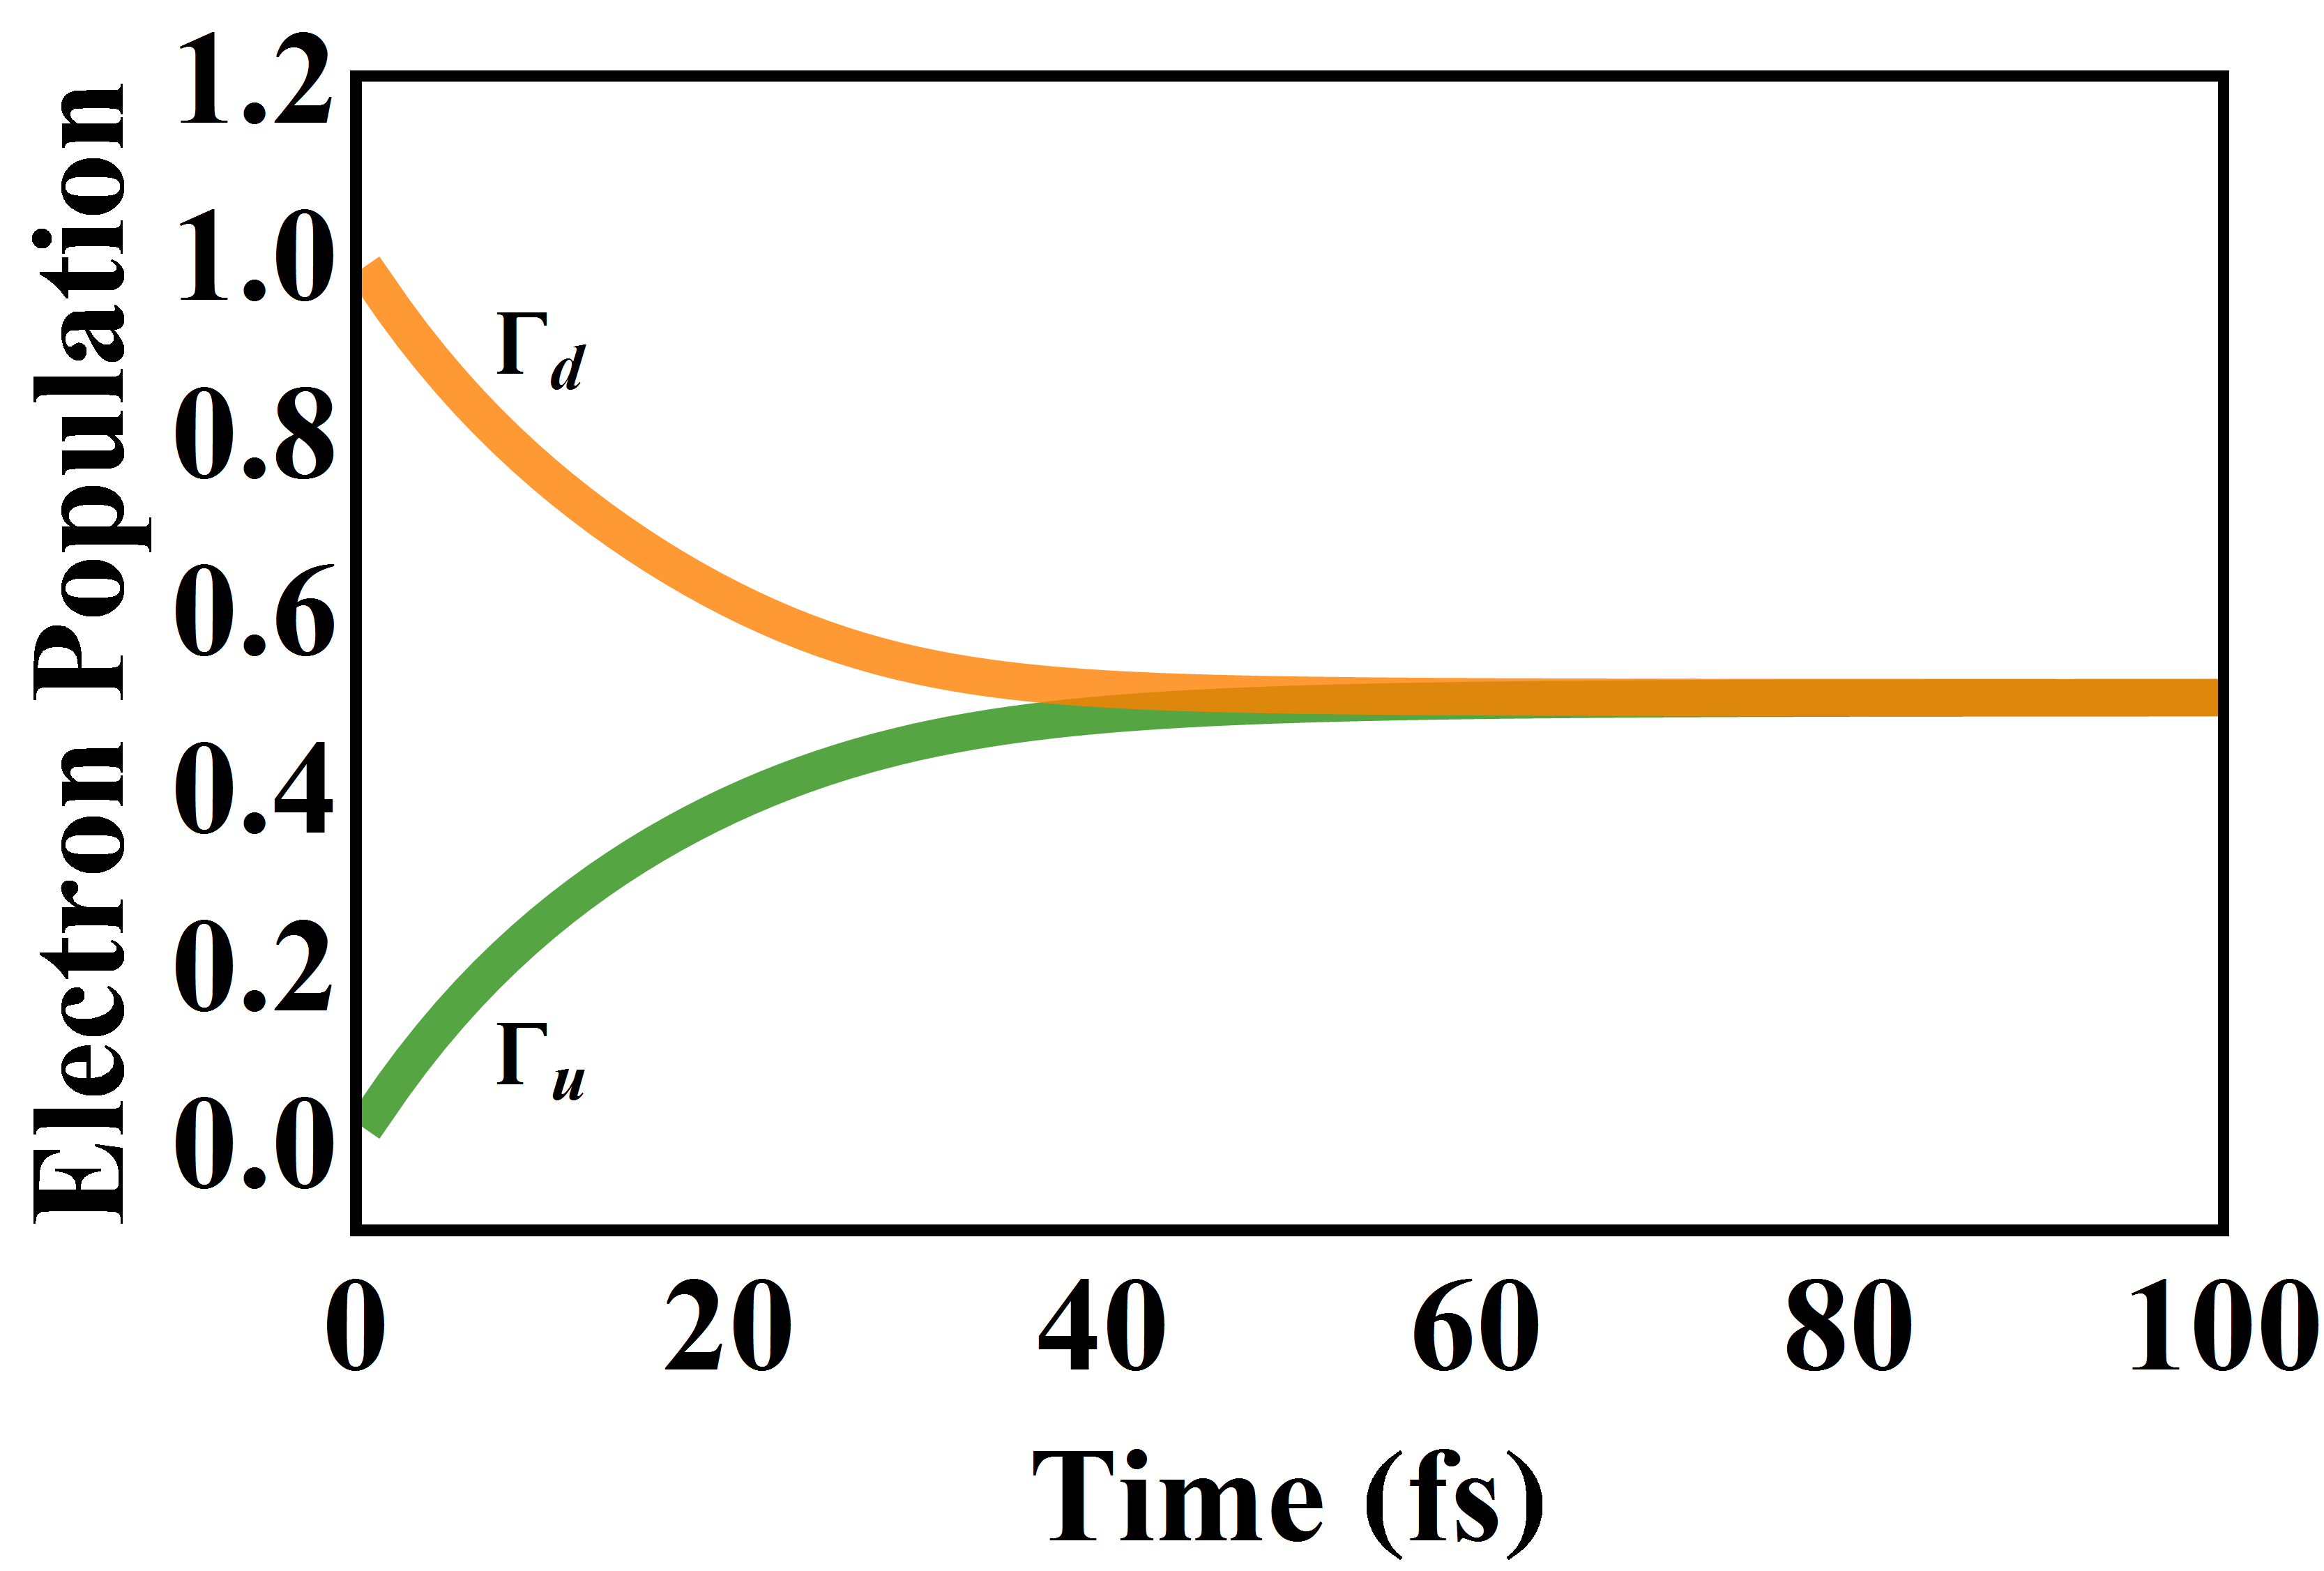
\includegraphics[scale=0.5]{./figures/pop42.png}
    \caption{电子占据数的含时演化}
    \label{fig:pop42}
\end{figure}

\section{4.2
激发态极化子的输运性质}\label{ux6fc0ux53d1ux6001ux6781ux5316ux5b50ux7684ux8f93ux8fd0ux6027ux8d28}

如果我们将电场作用下的极化子进行外界光的激发,情况又会如何?如图
(\ref{fig:epolaron2}a)
所示,我们在0飞秒时刻开始将电场作用于基态的极化子上,并且此时没有外界光激发的发生,此
时极化子处于第50个晶格的位置上。随着电场的作用,极化子开始在晶格上发生位移。在200飞秒
前,极化子已经运动到了100个晶格位置附近。如果在200飞秒开始加上强度为\(20\mu J/cm^2\)
的外界光激发的作用,此时,极化子处于100个晶格位置附近,到600飞秒时刻,外界光激发作用下
的极化子移动到第150格点的位置附近。显然的得到,外界光激发下的极化子在电场下的运动速
率小于基态的极化子在电场下的运动速率。同时,如果单独观察激发前后的运动随时间的变化,
它们都和时间呈线性关系。但是,计算发现,如果光强较小,例如,在图
(\ref{fig:epolaron2})中,我们使用\(0.2\mu J/cm^2\)的光强在200
飞秒时激发极化子。极化子的运动随时间的变化会呈一个非线性的关系。之所以会形成这样的运动
规律,我们猜测与极化子的自陷效应相关。

\begin{figure}[h!]
    \centering
    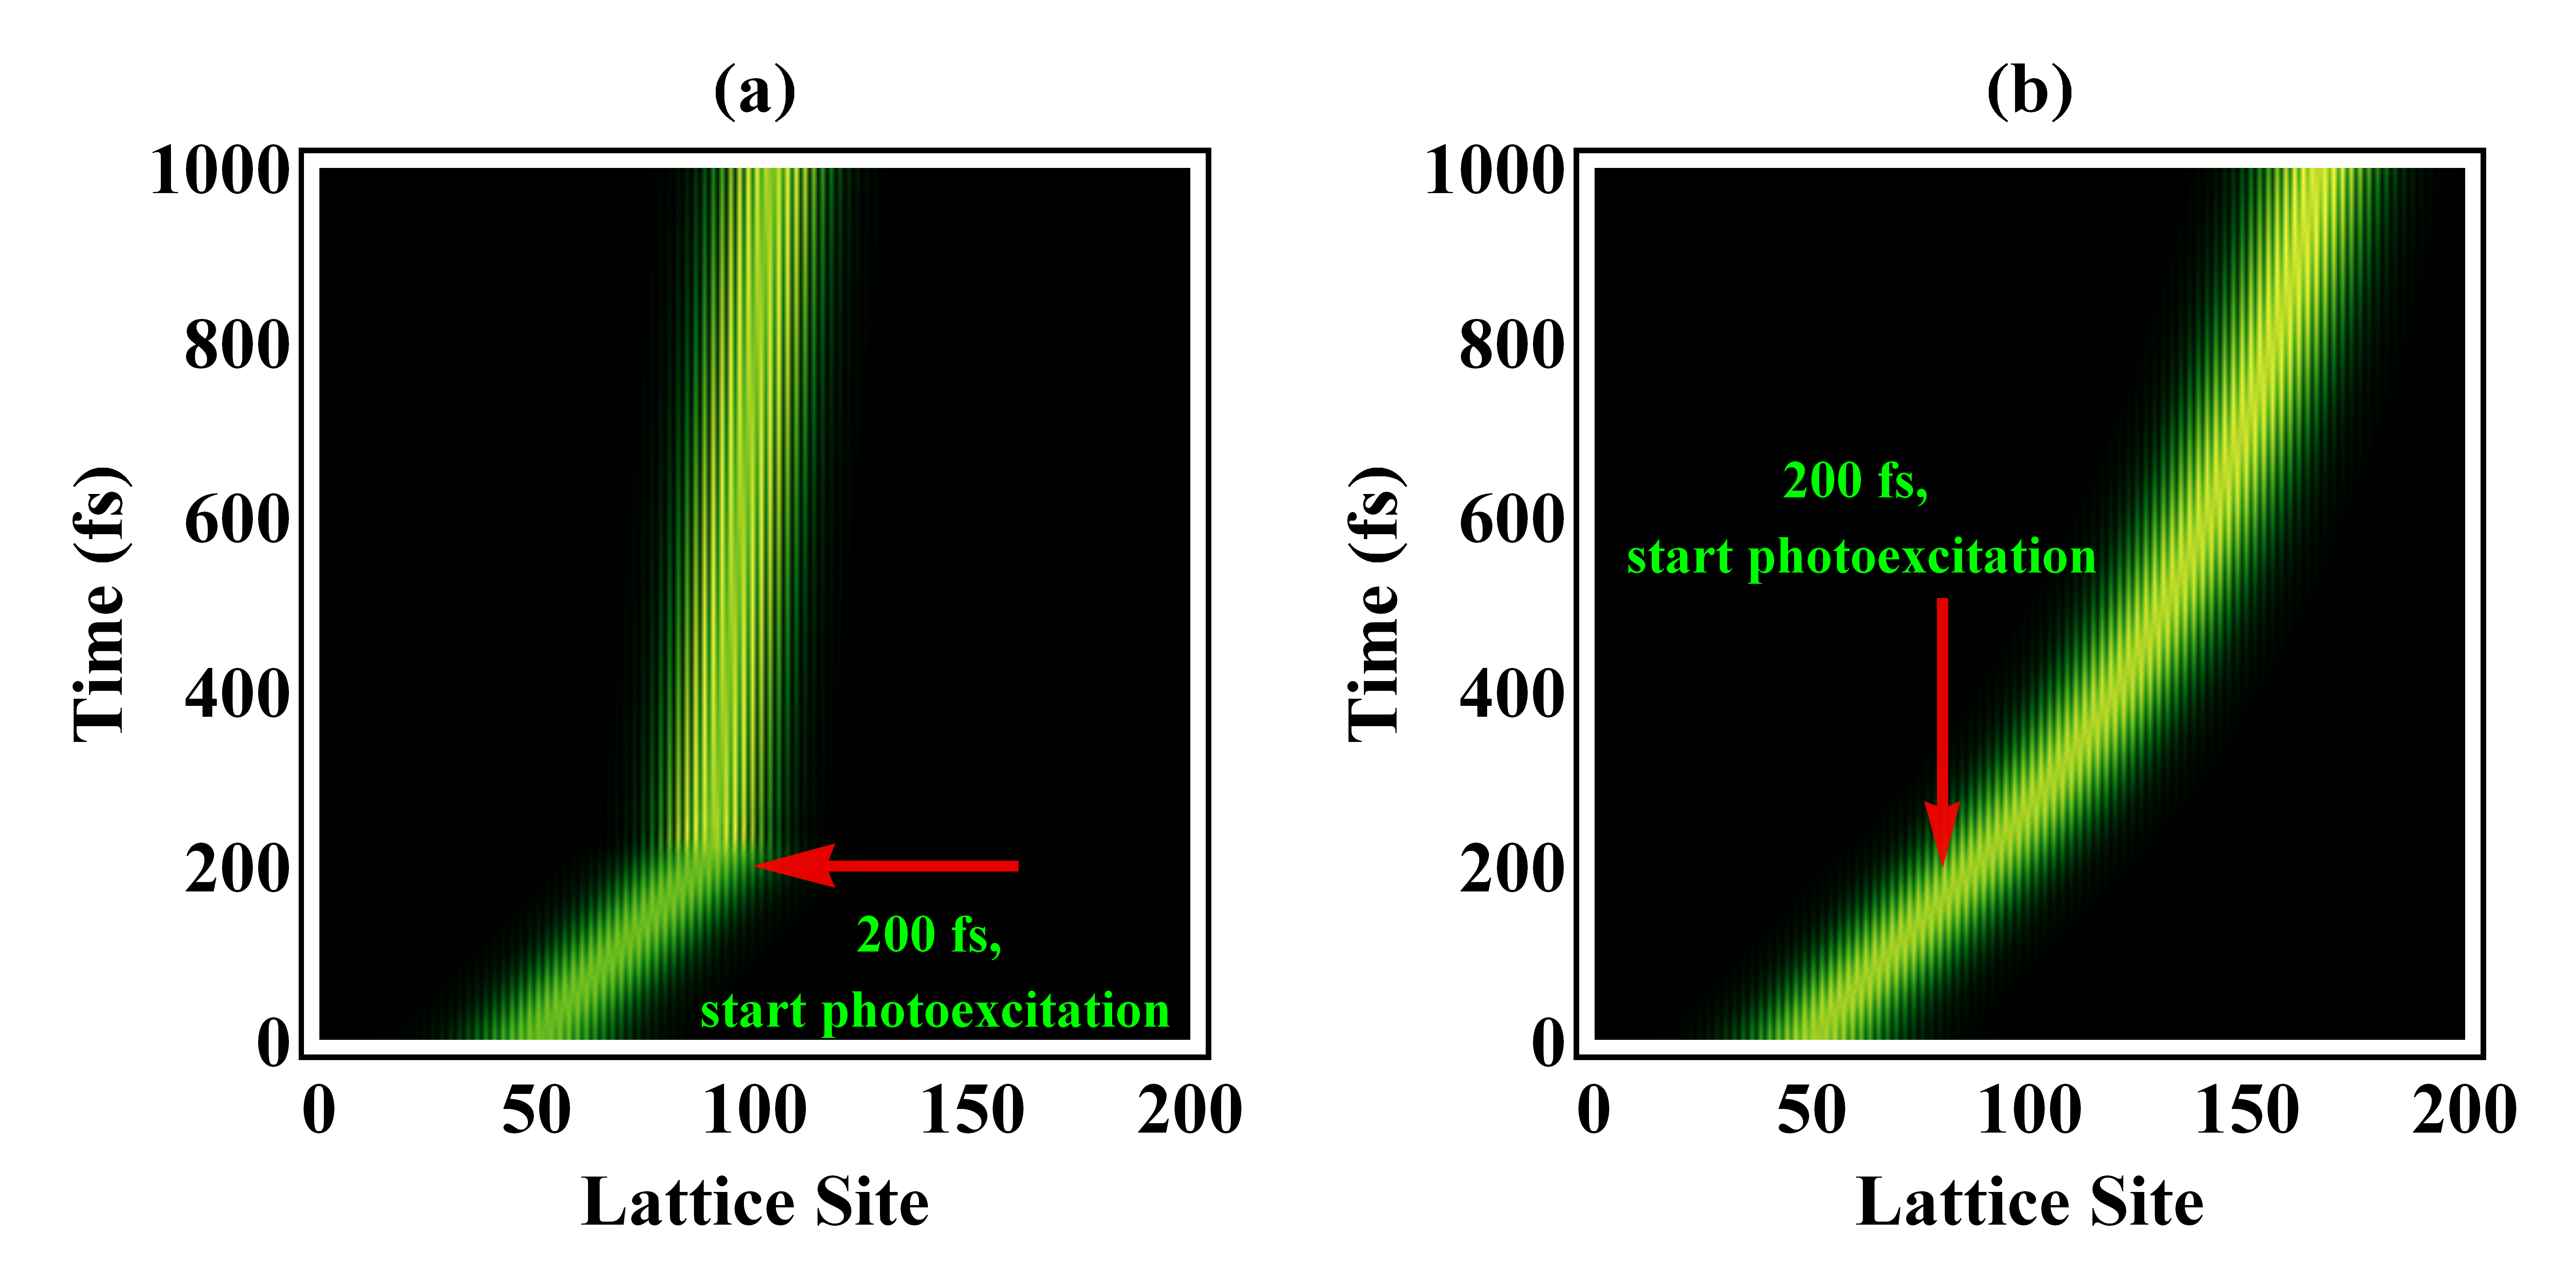
\includegraphics[scale=0.5]{./figures/epolaron2.png}
    \caption{外界光激发下的负极化子的运动: (a) 光强为$20\mu J/cm^2$; (b) 光强
    为$0.2\mu J/cm^2$ }
    \label{fig:epolaron2}
\end{figure}

自陷效应即:共轭聚合物分子中,共轭聚合物分子轨道上的电子分布发生变化会直接影响晶格的
结构,与此同时,晶格结构的变化也将促使电子在空间的重新分布,由此反复形成的新的晶格结
构和电子结构。对于共轭聚合物分子,在外界激发下最常见的晶格变化就是的畸变。所以,晶格
畸变的位置不仅代表了晶格运动的位置,同时也代表了极化子在晶格上的位置。从而,利用晶格
位型,我们可以直接得到整个聚合物链上极化子在晶格链上运动的直观图像,如图
(\ref{fig:e20chain})
所示。图中聚合物链的长度是200格点,图中展示从30个格点到150个格点的部分;小球代表原子
的位置,图例中的数值代表原子位移,单位是\AA。与图 (\ref{fig:epolaron2}a)
所描述的情况一样,初始时刻到200飞秒之间只有电场的作用,晶格畸变的位置从链的左端移动到
了中部。而在200飞秒时刻加上\(20\mu J/cm^2\)的外界光强,从400飞秒
的晶格畸变可以看出,晶格畸变代表的原子之间偏离平衡位置的位移减小
。同时,这一段晶格畸变的部分在400飞秒到1000飞秒内发生了一段非常小的移动,表明被激发状态
下的极化子自陷效应引起的晶格运动变慢了,其运动规律与图
(\ref{fig:epolaron2}a)所描述的极化子运动相对应。而图(\ref{fig:e02chain})给出了与图
(\ref{fig:epolaron2}a)相对应的晶格运动,在200飞秒加入\(0.2\mu J/cm^2\)的光强导致极化子被
激发。400 飞秒时,与\(20\mu J/cm^2\)
的情况不同,晶格的运动到了接近150个晶格的位置。表明弱光强对极化子运动速率的改变响应
较慢。直到1000
飞秒时,晶格畸变的程度相比较400飞秒时出现了较为明显的变化,其表征的原子之间的平衡位置偏
离减小了。这说明,在400飞秒到1000
飞秒之间,极化子受到光激发的影响一直在进行,此时的极化子还没有因为光激发而处于新的稳定
状态。因此,我们可以知道,极化子在图 (\ref{fig:epolaron2}b)
中的位置随时间呈非线性的改变是由于弱光强下,激发态极化子还来不及形成新的稳定状态,导
致自陷效应引起的晶格畸变一直处于变化当中。综上所述,稳定状态的极化子,不论激发态还是
基态,在电场中运动时的位置随时间的变化呈线性关系。非稳态的极化子在电场中运动时的位置
随时间的变化并非线性,且被激发的程度越大,极化子的运动速度就越慢。

\begin{figure}[h!]
    \centering
    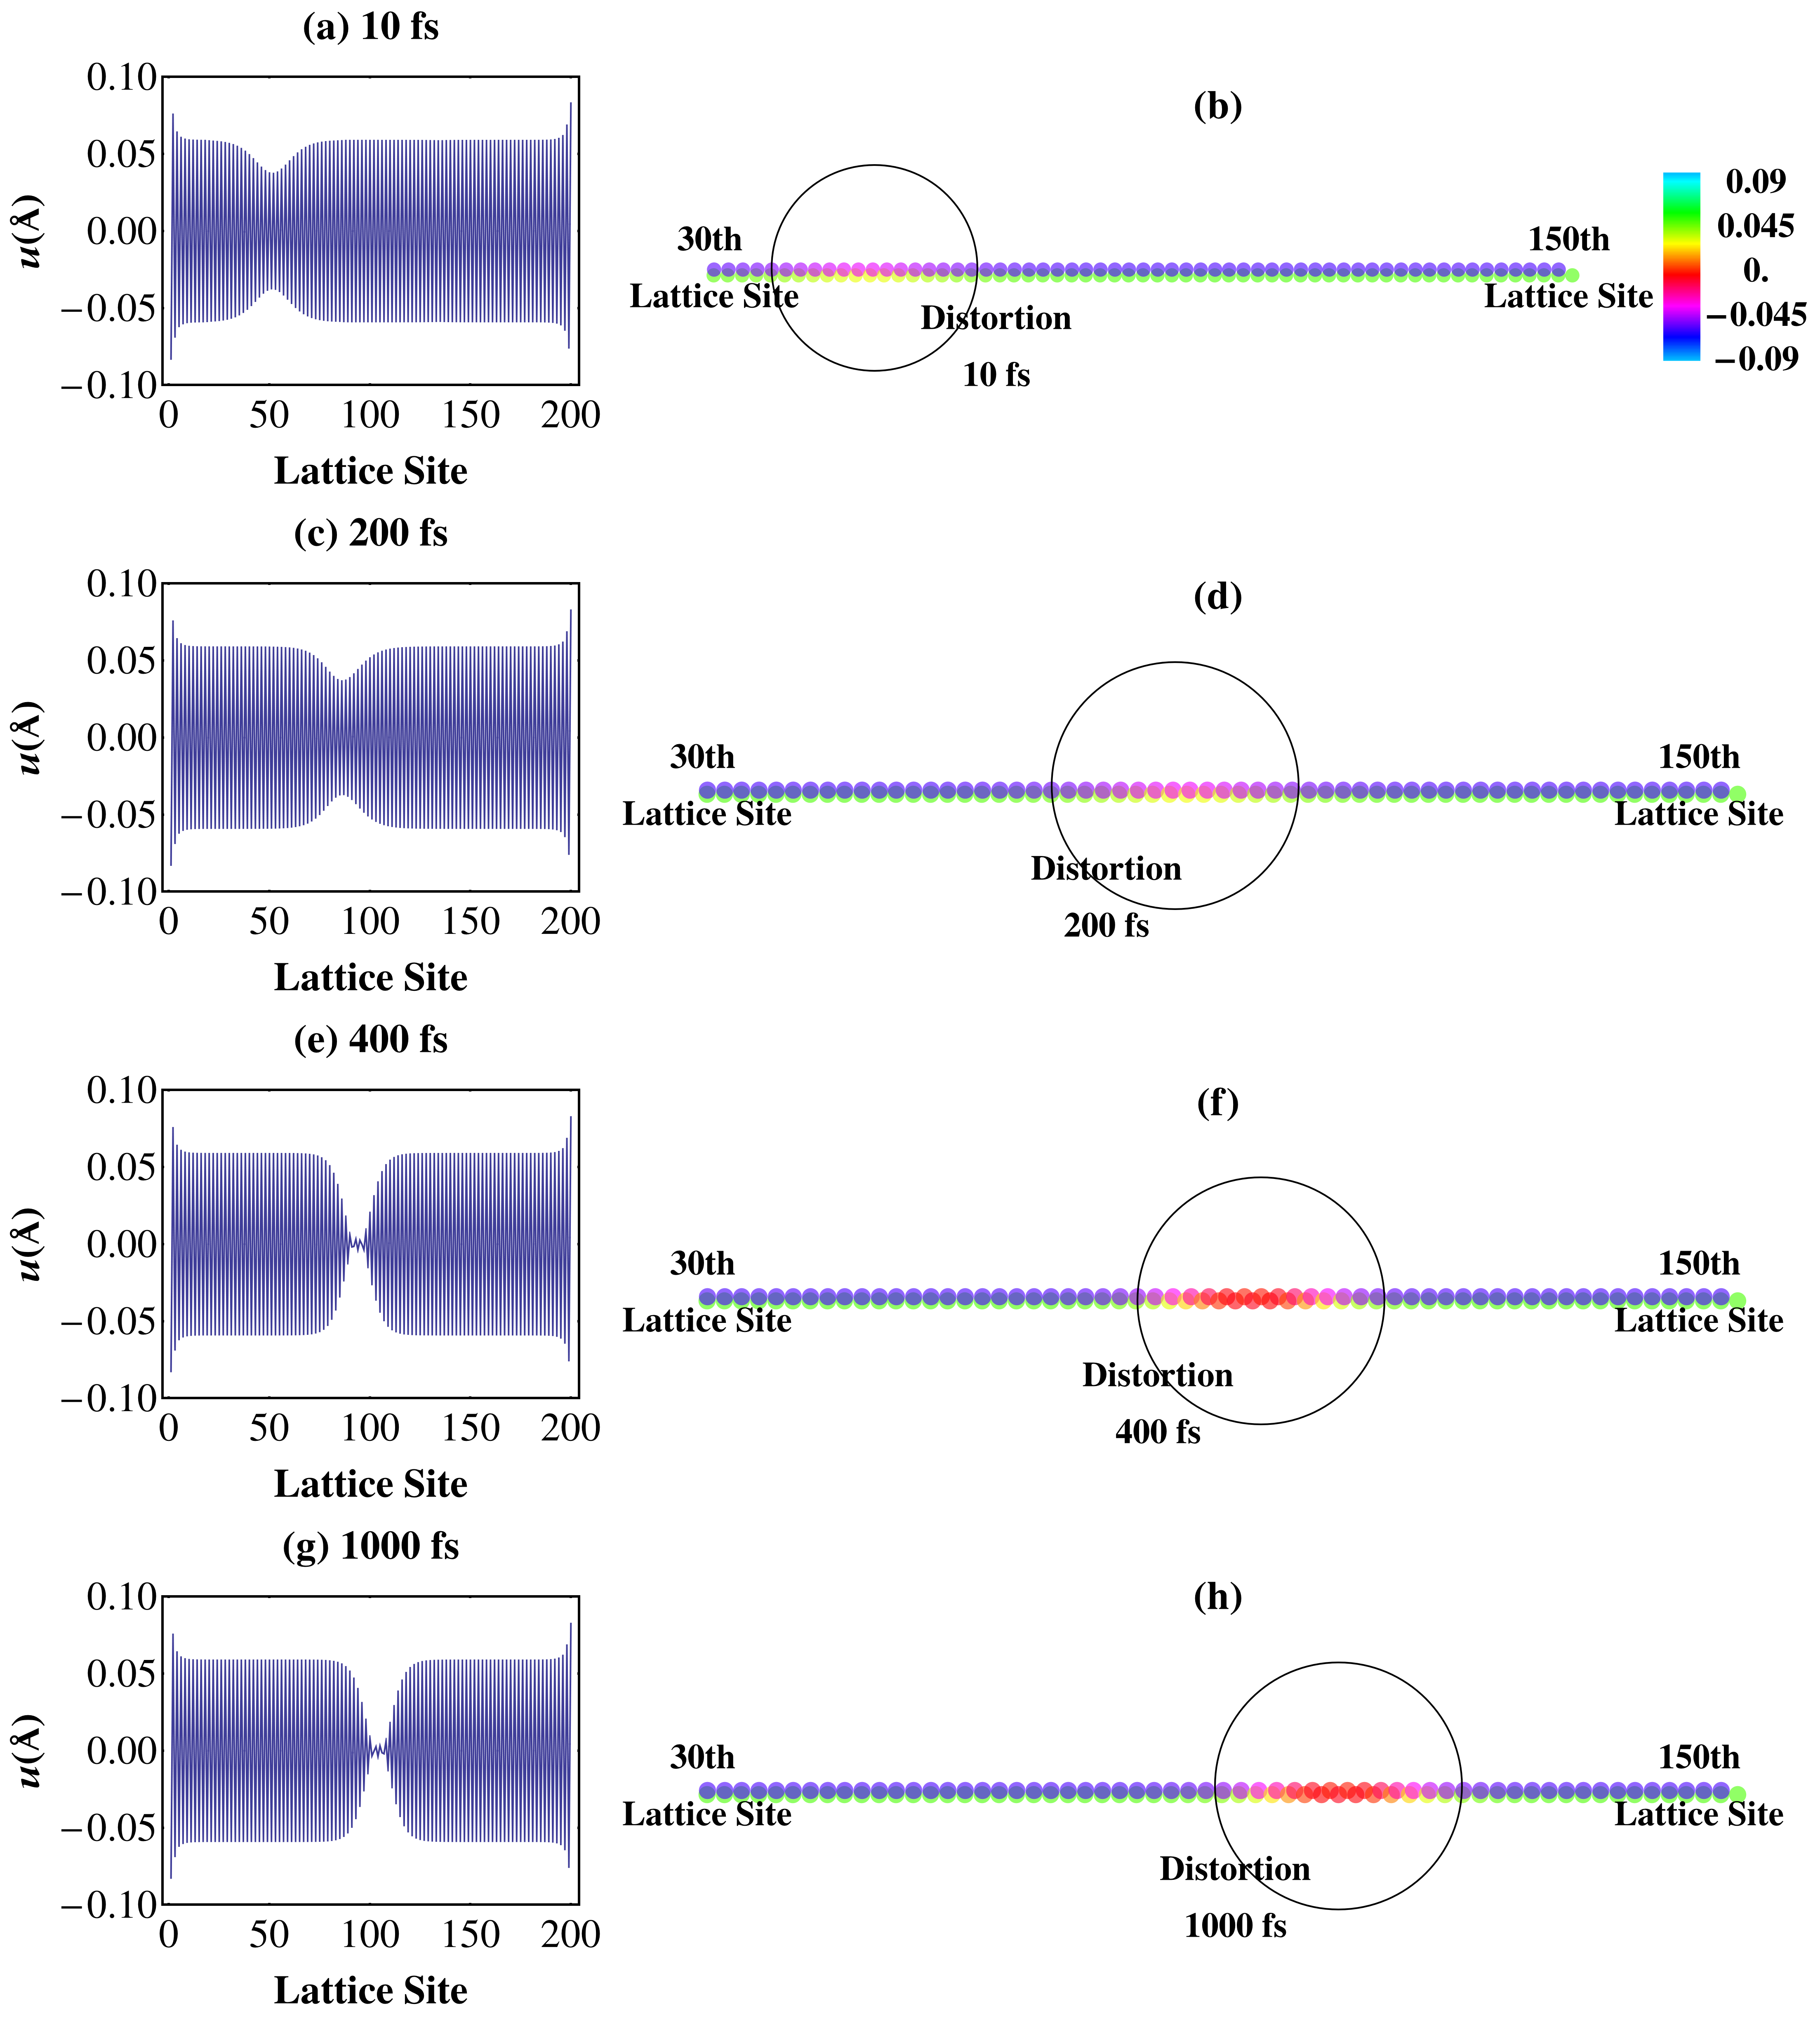
\includegraphics[scale=0.3]{./figures/chfigoutStraight.png}
    \caption{在光强为$20\mu J/cm^2$的外界光作用下的晶格畸变的运动}
    \label{fig:e20chain}
\end{figure}

\begin{figure}[h!]
    \centering
    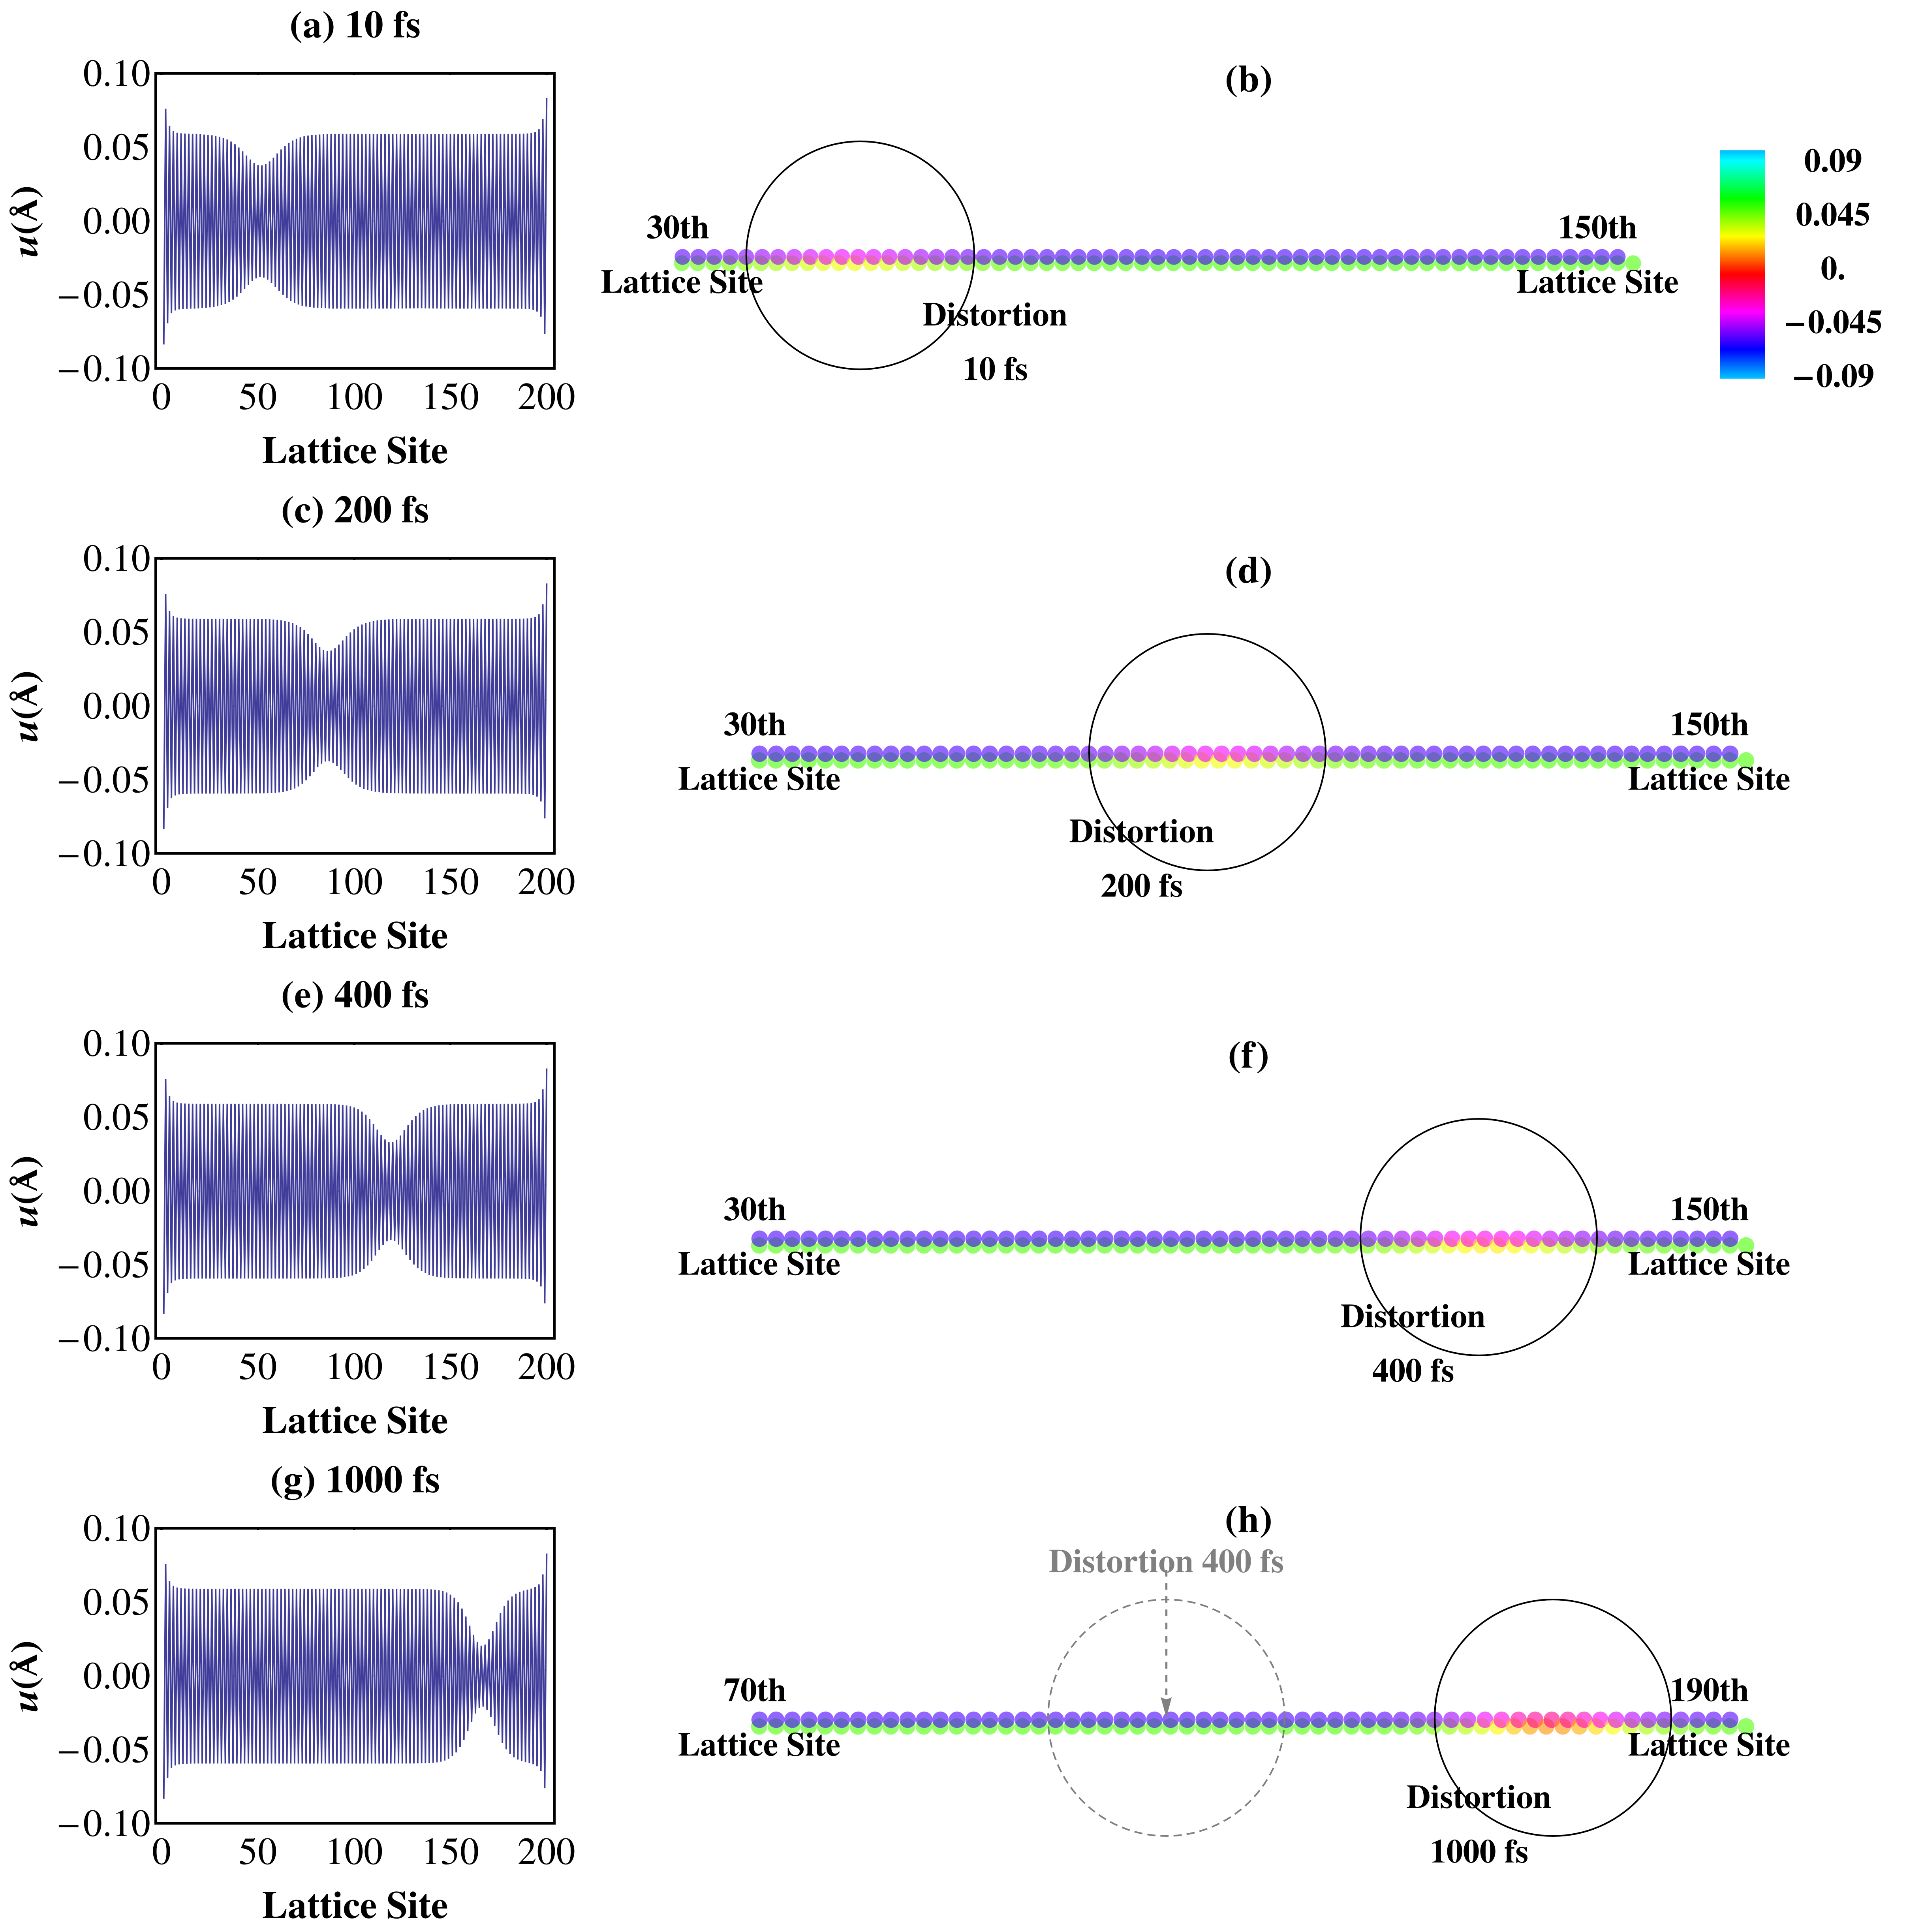
\includegraphics[scale=0.3]{./figures/chfigweakoutStraight.png}
    \caption{在光强为$20\mu J/cm^2$的外界光作用下的晶格畸变的运动}
    \label{fig:e02chain}
\end{figure}

激发程度的大小可以由能级结构来表征。如果我们观察外界光激发作用下极化子在电场中的运动
的整个过程中能级对应的电子占据数变化,如图(\ref{fig:pop20})
所示,在初始的0飞秒时刻,基态的极化子开始受到电场的作用而,上局域能级的电子占据数为0,
随着电场的作用,200飞秒内,电子占据数没有发生变化而保持为0,代表了极化子的能级结构没有
发生改变,即极化子仍然处于基态。200飞秒时刻,开始加入光强为\(20\mu J/cm^2\)(a)和
\(0.2\mu J/cm^2\)(b)的外界光激发的作用,可以看到,在200飞秒到400飞秒时刻内,对于强光作用下
的上局域能级的电子占据数发生了明显的变化,其数值从0迅速地上升到了 0.5
,即极化子的能级结构发生了迅速地变化,导致原本处于基态的极化子不再处于基态而形成了新
的激发状态。在弱光强的作用下,极化子能级结构的变化不明显且在200飞秒内也没有达到新的稳
定状态。

\begin{figure}[h!]
    \centering
    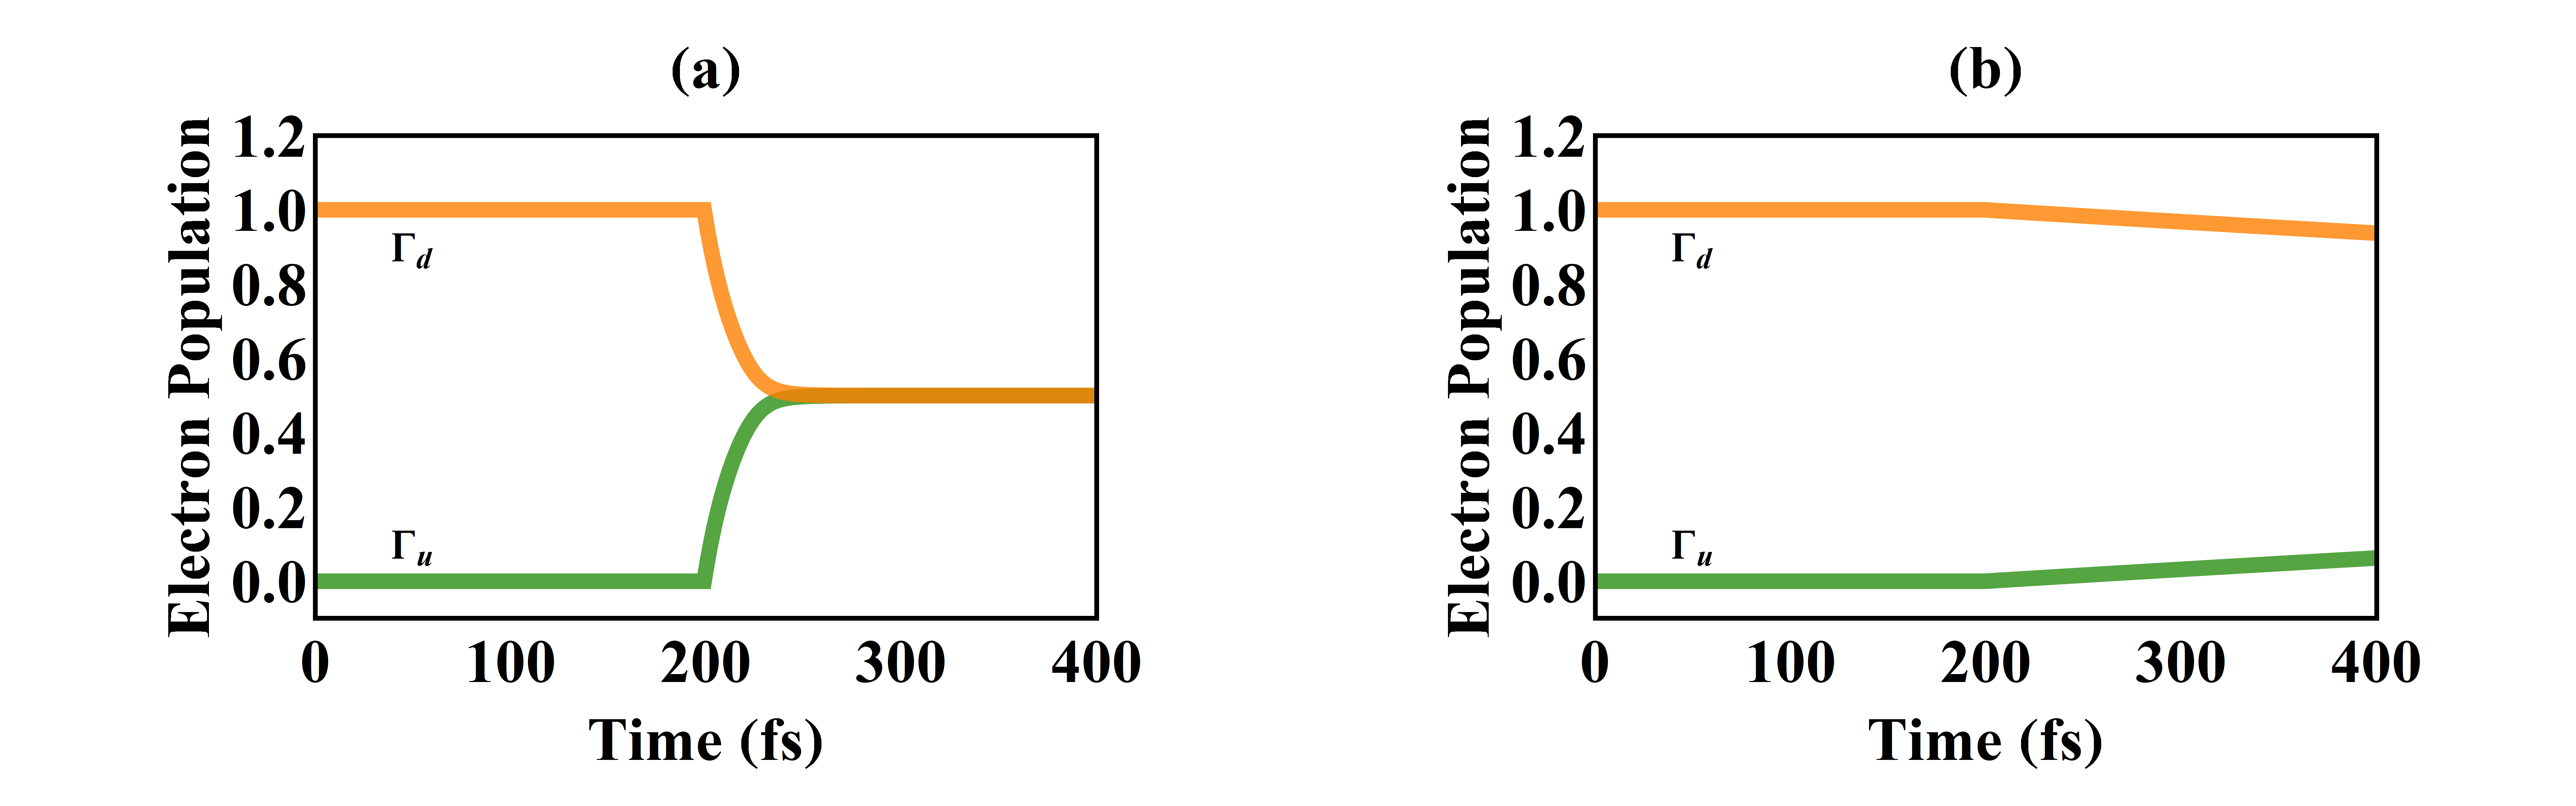
\includegraphics[scale=0.5]{./figures/population20.png}
    \caption{电子占据数的含时变化: (a) 外界光强为$20\mu J/cm^2$; (b) 外界光强为
    $0.2\mu J/cm^2$}
    \label{fig:pop20}
\end{figure}

\clearpage
\clearpage\pagestyle{empty}\mbox{}\clearpage

\pagestyle{fancy}

\chapter{结论}\label{ux7ed3ux8bba}

本文利用分子动力学方法揭示了在共轭聚合物太阳能电池受到外界光激发后,激子的形成过程分为两部
分,激子的局域和激子的弛豫。外界光的激发引起了聚合物分子中的电子受激跃迁,诱发了激子
的局域: 激子晶格位的局域与电子态的局域。在激子的局域过程中
,激子的能量发生剧烈振荡。在激子形成的过程中完成电子跃迁和局域后,共轭聚合物分子进入激子的弛豫过
程,在此过程中,激子在保持局域的同时,激子的能量也按照固定的周期缓缓振荡,最终收敛,
形成激子。此外,本文也揭示了在激子形成局域过程中,外界光强对激子局域的时间的影响,发
现外界光强的增大,不仅能缩短激子形成过程中电子激发的时间,也将缩短激子局域的时间,并
最终缩短激子形成的时间。

共轭聚合物太阳能电池的原理也涉及到载流子输运,该输运也在外界光强的作用下进行。本文通过
传统分子动力学的方法研究了光激发下的载流子输运,发现外界光强的作用可能导致输运中的载
流子被激发。而激发后的载流子输运速度明显低于基态载流子的输运速度。减速的原因是由于自
陷效应引起的晶格运动的减速影响了极化子本身的输运速率。输运速度的降低可能会降低载流子
被输运到电极的几率,最终影响太阳能电池工作的效率。

\clearpage
\clearpage\pagestyle{empty}\mbox{}\clearpage
\begin{center}
\Huge \textbf{参考文献}
\end{center}

\lhead{} \chead{参考文献} \rhead{} \pagestyle{plain}
\addcontentsline{toc}{chapter}{参考文献} \setlength{\parindent}{0em}

{[}1{]} 孙 鑫. 高聚物中的孤子和极化子{[}M{]}. 四川教育出版社, 1987

{[}2{]} Sachdev V., Kumar R., Singh A., Kumar S., Mehra R. Electrically
Conducting Polymers: An Overview{[}J{]}. Solid State Phenomena, 1997,
55: 104--109.
doi:\href{http://dx.doi.org/10.4028/www.scientific.net/SSP.55.104}{10.4028/www.scientific.net/SSP.55.104}

{[}3{]} Hotta C. Theoretical classification of two-dimensional organic
conductors{[}J{]}. Physica B: Condensed Matter, 2003, 329-333:
1164--1165.
doi:\href{http://dx.doi.org/10.1016/S0921-4526(02)02084-7}{10.1016/S0921-4526(02)02084-7}

{[}4{]} Dupuis N., Yakovenko V.M. Sign reversals of the quantum Hall
effect and helicoidal magnetic-field-induced spin-density waves in
organic conductors{[}J{]}. Physica B: Condensed Matter, 1999, 259-261:
1013--1014.
doi:\href{http://dx.doi.org/10.1016/S0921-4526(98)01056-4}{10.1016/S0921-4526(98)01056-4}

{[}5{]} Peierls R.E. Quantum Theory of Solids{[}M{]}. OXFORD UNIVERSITY
PRESS, 1955

{[}6{]} Wang Z., Wu C., Sun X. A criterion for two kinds of Peierls
transitions{[}J{]}. Chinese Physics Letters, 1985, 2(3): 141--144.
doi:\href{http://dx.doi.org/10.1088/0256-307X/2/3/012}{10.1088/0256-307X/2/3/012}

{[}7{]} Shirakawa H., Louis E.J., MacDiarmid A.G., Chiang C.K., Heeger
A.J. Synthesis of electrically conducting organic polymers: Halogen
derivatives of polyacetylene, (CH) x{[}J{]}. Journal of the Chemical
Society, Chemical Communications, 1977(16): 578.
doi:\href{http://dx.doi.org/10.1039/c39770000578}{10.1039/c39770000578}

{[}8{]} 诸平, 张文根. 白川英树与导电聚合物发现力学纪学{[}J{]}. 2003,
18(1): 60--62.

{[}9{]} Lippe J., Holze R. Electrochemical in-situ conductivity and
polaron concentration measurements at selected conducting
polymers{[}J{]}. Synthetic Metals, 1991, 43(1-2): 2927--2930.
doi:\href{http://dx.doi.org/10.1016/0379-6779(91)91208-R}{10.1016/0379-6779(91)91208-R}

{[}10{]} A Bernanose, Comte M., Vouaux P. A new method of emission of
light by certain organic compounds{[}J{]}. J. Chim. Phys, 1953, 50:
64--68.

{[}11{]} Bernanose A., Vouaux P. Organic electroluminescence type of
emission{[}J{]}. J. Chim. Phys, 1953, 50: 261.

{[}12{]} Bernanose A. J. Chim. Phys., 1955, 52: 396.

{[}13{]} Bernanose A., Vouaux P. J. Chim. Phys., 1955, 52: 509.

{[}14{]} Kallmann H., Pope M. Bulk Conductivity in Organic
Crystals{[}J{]}. Nature, 1960, 186(4718): 31--33.
doi:\href{http://dx.doi.org/10.1038/186031a0}{10.1038/186031a0}

{[}15{]} Pope M., Kallmann H.P., Magnante P. Electroluminescence in
Organic Crystals{[}J{]}. The Journal of Chemical Physics, 1963, 38(8):
2042. doi:\href{http://dx.doi.org/10.1063/1.1733929}{10.1063/1.1733929}

{[}16{]} Kallmann H., Pope M. Positive Hole Injection into Organic
Crystals{[}J{]}. The Journal of Chemical Physics, 1960, 32(1): 300.
doi:\href{http://dx.doi.org/10.1063/1.1700925}{10.1063/1.1700925}

{[}17{]} Mark P., Helfrich W. Space-Charge-Limited Currents in Organic
Crystals{[}J{]}. Journal of Applied Physics, 1962, 33(1): 205.
doi:\href{http://dx.doi.org/10.1063/1.1728487}{10.1063/1.1728487}

{[}18{]} Helfrich W., Schneider W. Recombination Radiation in Anthracene
Crystals{[}J{]}. Physical Review Letters, 1965, 14(7): 229--231.
doi:\href{http://dx.doi.org/10.1103/PhysRevLett.14.229}{10.1103/PhysRevLett.14.229}

{[}19{]} Partridge R. Electroluminescence from polyvinylcarbazole films:
1. Carbazole cations{[}J{]}. Polymer, 1983, 24(6): 733--738.
doi:\href{http://dx.doi.org/10.1016/0032-3861(83)90012-5}{10.1016/0032-3861(83)90012-5}

{[}20{]} Partridge R. Electroluminescence from polyvinylcarbazole films:
2. Polyvinylcarbazole films containing antimony pentachloride{[}J{]}.
Polymer, 1983, 24(6): 739--747.
doi:\href{http://dx.doi.org/10.1016/0032-3861(83)90013-7}{10.1016/0032-3861(83)90013-7}

{[}21{]} Partridge R. Electroluminescence from polyvinylcarbazole films:
3. Electroluminescent devices{[}J{]}. Polymer, 1983, 24(6): 748--754.
doi:\href{http://dx.doi.org/10.1016/0032-3861(83)90014-9}{10.1016/0032-3861(83)90014-9}

{[}22{]} Partridge R. Electroluminescence from polyvinylcarbazole films:
4. Electroluminescence using higher work function cathodes{[}J{]}.
Polymer, 1983, 24(6): 755--762.
doi:\href{http://dx.doi.org/10.1016/0032-3861(83)90015-0}{10.1016/0032-3861(83)90015-0}

{[}23{]} Tang C.W., VanSlyke S.A. Organic electroluminescent
diodes{[}J{]}. Applied Physics Letters, 1987, 51(12): 913.
doi:\href{http://dx.doi.org/10.1063/1.98799}{10.1063/1.98799}

{[}24{]} Burroughes J.H., Bradley D.D.C., Brown A.R., Marks R.N., Mackay
K., Friend R.H., Burns P.L., Holmes A.B. Light-emitting diodes based on
conjugated polymers{[}J{]}. Nature, 1990, 347(6293): 539--541.
doi:\href{http://dx.doi.org/10.1038/347539a0}{10.1038/347539a0}

{[}25{]} Baldo M.A., O'Brien D.F., You Y., Shoustikov A., Sibley S.,
Thompson M., Forrest S.R. Highly efficient phosphorescent emission from
organic electroluminescent devices{[}J{]}. Nature, 1988, 395: 151--154.

{[}26{]} Cao Y., Parker I.D., Yu G., Zhang C., Heeger A.J. Improved
quantum efficiency for electroluminescence in semiconducting
polymers{[}J{]}. Nature, 1999, 397: 414--417.

{[}27{]} Zhang S.M. Sem. Opto., 2003, 24: 84.

{[}28{]} Tsumura A., Koezuka H., Ando T. Macromolecular electronic
device: Field-effect transistor with a polythiophene thin film{[}J{]}.
Applied Physics Letters, 1986, 49(18): 1210.
doi:\href{http://dx.doi.org/10.1063/1.97417}{10.1063/1.97417}

{[}29{]} Horowitz G., Kouki F., Spearman P., Fichou D., Nogues C., Pan
X., Garnier F. Evidence for n-type conduction in a perylene
tetracarboxylic diimide derivative{[}J{]}. Advanced Materials, 1996,
8(3): 242--245.
doi:\href{http://dx.doi.org/10.1002/adma.19960080312}{10.1002/adma.19960080312}

{[}30{]} Ghosh A.K., Morel D.L., Feng T., Shaw R.F., Rowe C.A.
Photovoltaic and rectification properties of Al∕Mg phthalocyanine∕Ag
Schottky-barrier cells{[}J{]}. Journal of Applied Physics, 1974, 45(1):
230. doi:\href{http://dx.doi.org/10.1063/1.1662965}{10.1063/1.1662965}

{[}31{]} Kallmann H., Pope M. Photovoltaic Effect in Organic
Crystals{[}J{]}. The Journal of Chemical Physics, 1959, 30(2): 585--586.
doi:\href{http://dx.doi.org/10.1063/1.1729992}{10.1063/1.1729992}

{[}32{]} Shirakawa H., Ikeda S. Preparation and morphology of
as-prepared and highly stretch-aligned polyacetylene{[}J{]}. Synthetic
Metals, 1980, 1(2): 175--184.
doi:\href{http://dx.doi.org/10.1016/0379-6779(80)90008-9}{10.1016/0379-6779(80)90008-9}

{[}33{]} Shirakawa H., Louis E.J., MacDiarmid A.G., Chiang C.K., Heeger
A.J. Synthesis of electrically conducting organic polymers: Halogen
derivatives of polyacetylene, (CH) x{[}J{]}. Journal of the Chemical
Society, Chemical Communications, 1977(16): 578.
doi:\href{http://dx.doi.org/10.1039/c39770000578}{10.1039/c39770000578}

{[}34{]} Chiang C., Fincher C., Park Y., Heeger A., Shirakawa H., Louis
E., Gau S., MacDiarmid A. Electrical Conductivity in Doped
Polyacetylene{[}J{]}. Physical Review Letters, 1977, 39(17): 1098--1101.
doi:\href{http://dx.doi.org/10.1103/PhysRevLett.39.1098}{10.1103/PhysRevLett.39.1098}

{[}35{]} Weinberger B., Akhtar M., Gau S. Polyacetylene photovoltaic
devices{[}J{]}. Synthetic Metals, 1982, 4(3): 187--197.
doi:\href{http://dx.doi.org/10.1016/0379-6779(82)90012-1}{10.1016/0379-6779(82)90012-1}

{[}36{]} Haugeneder A., Neges M., Kallinger C., Spirkl W., Lemmer U.,
Feldmann J., Scherf U., Harth E., Gugel A., Mullen K. Exciton diffusion
and dissociation in conjugated polymer/fullerene blends and
heterostructures{[}J{]}. Physical Review B, 1999, 59(23): 15346--15351.
doi:\href{http://dx.doi.org/10.1103/PhysRevB.59.15346}{10.1103/PhysRevB.59.15346}

{[}37{]} Stubinger T., Brutting W. Exciton diffusion and optical
interference in organic donor--acceptor photovoltaic cells{[}J{]}.
Journal of Applied Physics, 2001, 90(7): 3632.
doi:\href{http://dx.doi.org/10.1063/1.1394920}{10.1063/1.1394920}

{[}38{]} Theander M., Yartsev A., Zigmantas D., Sundstrom V., Mammo W.,
Andersson M., Inganas O. Photoluminescence quenching at a
polythiophene/C60 heterojunction{[}J{]}. Physical Review B, 2000,
61(19): 12957--12963.

{[}39{]} Maniloff E., Klimov V., McBranch D. Intensity-dependent
relaxation dynamics and the nature of the excited-state species in
solid-state conducting polymers{[}J{]}. Physical Review B, 1997, 56(4):
1876--1881.
doi:\href{http://dx.doi.org/10.1103/PhysRevB.56.1876}{10.1103/PhysRevB.56.1876}

{[}40{]} Vacar D., Maniloff E., McBranch D., Heeger A. Charge-transfer
range for photoexcitations in conjugated polymer/fullerene bilayers and
blends{[}J{]}. Physical Review B, 1997, 56(8): 4573--4577.
doi:\href{http://dx.doi.org/10.1103/PhysRevB.56.4573}{10.1103/PhysRevB.56.4573}

{[}41{]} Tang C.W. Two-layer organic photovoltaic cell{[}J{]}. Applied
Physics Letters, 1986, 48(2): 183.
doi:\href{http://dx.doi.org/10.1063/1.96937}{10.1063/1.96937}

{[}42{]} Sariciftci N.S., Smilowitz L., Heeger A.J., Wudl F.
Photoinduced Electron Transfer from a Conducting Polymer to
Buckminsterfullerene{[}J{]}. Science, 1992, 258(5087): 1474--1476.
doi:\href{http://dx.doi.org/10.1126/science.258.5087.1474}{10.1126/science.258.5087.1474}

{[}43{]} Smilowitz L., Sariciftci N., Wu R., Gettinger C., Heeger A.,
Wudl F. Photoexcitation spectroscopy of conducting-polymer--C60
composites: Photoinduced electron transfer{[}J{]}. Physical Review B,
1993, 47(20): 13835--13842.
doi:\href{http://dx.doi.org/10.1103/PhysRevB.47.13835}{10.1103/PhysRevB.47.13835}

{[}44{]} Lee C., Yu G., Moses D., Pakbaz K., Zhang C., Sariciftci N.,
Heeger A., Wudl F. Sensitization of the photoconductivity of conducting
polymers by C60: Photoinduced electron transfer{[}J{]}. Physical Review
B, 1993, 48(20): 15425--15433.
doi:\href{http://dx.doi.org/10.1103/PhysRevB.48.15425}{10.1103/PhysRevB.48.15425}

{[}45{]} Morita S., Zakhidov A.A., Yoshino K. Doping effect of
buckminsterfullerene in conducting polymer: Change of absorption
spectrum and quenching of luminescene{[}J{]}. Solid State
Communications, 1992, 82(4): 249--252.
doi:\href{http://dx.doi.org/10.1016/0038-1098(92)90636-N}{10.1016/0038-1098(92)90636-N}

{[}46{]} Yoshino K., Yin X.H., Muro K., Kiyomatsu S., Morita S.,
Zakhidov A.A., Noguchi T., Ohnishi T. Marked Enhancement of
Photoconductivity and Quenching of Luminescence in
Poly(2,5-dialkoxy-p-phenylene vinylene) upon C \(_{\textrm{60}}\)
Doping{[}J{]}. Japanese Journal of Applied Physics, 1993, 32(Part 2, No.
3A): L357--L360.
doi:\href{http://dx.doi.org/10.1143/JJAP.32.L357}{10.1143/JJAP.32.L357}

{[}47{]} Liang W.Y. Excitons{[}J{]}. Physics Education, 1970, 5(4):
226--228.
doi:\href{http://dx.doi.org/10.1088/0031-9120/5/4/003}{10.1088/0031-9120/5/4/003}

{[}48{]} Yang C., Heeger A. Morphology of composites of semiconducting
polymers mixed with C60{[}J{]}. Synthetic Metals, 1996, 83(2): 85--88.
doi:\href{http://dx.doi.org/10.1016/S0379-6779(97)80058-6}{10.1016/S0379-6779(97)80058-6}

{[}49{]} Scharber M., Sariciftci N. Efficiency of bulk-heterojunction
organic solar cells{[}J{]}. Progress in Polymer Science, 2013, 38(12):
1929--1940. 

{[}50{]} Guo J., Ohkita H., Benten H., Ito S. Charge Generation and
Recombination Dynamics in Poly(3-hexylthiophene)/Fullerene Blend Films
with Different Regioregularities and Morphologies{[}J{]}. Journal of the
American Chemical Society, 2010, 132(17): 6154--6164.
doi:\href{http://dx.doi.org/10.1021/ja100302p}{10.1021/ja100302p}

{[}51{]} Tautz R., Da Como E., Wiebeler C., Soavi G., Dumsch I.,
Frohlich N., Grancini G., Allard S., Scherf U., Cerullo G., Schumacher
S., Feldmann J. Charge Photogeneration in Donor--Acceptor Conjugated
Materials: Influence of Excess Excitation Energy and Chain
Length{[}J{]}. Journal of the American Chemical Society, 2013, 135(11):
4282--4290.
doi:\href{http://dx.doi.org/10.1021/ja309252a}{10.1021/ja309252a}

{[}52{]} Gonzalez S.R., Ie Y., Aso Y., Lopez Navarrete J.T., Casado J.
The Frontiers of Quinoidal Stability in Long Oligothiophenes: Raman
Spectra of Dicationic Polaron Pairs{[}J{]}. Journal of the American
Chemical Society, 2011, 133(41): 16350--16353.
doi:\href{http://dx.doi.org/10.1021/ja2061903}{10.1021/ja2061903}

{[}53{]} Banerji N., Cowan S., Leclerc M., Vauthey E., Heeger A.J.
Exciton Formation, Relaxation, and Decay in PCDTBT{[}J{]}. Journal of
the American Chemical Society, 2010, 132(49): 17459--17470.
doi:\href{http://dx.doi.org/10.1021/ja105290e}{10.1021/ja105290e}

{[}54{]} Banerji N., Cowan S., Vauthey E., Heeger A.J. Ultrafast
Relaxation of the Poly(3-hexylthiophene) Emission Spectrum{[}J{]}. The
Journal of Physical Chemistry C, 2011, 115(19): 9726--9739.
doi:\href{http://dx.doi.org/10.1021/jp1119348}{10.1021/jp1119348}

{[}55{]} Devižis A., Serbenta A., Meerholz K., Hertel D., Gulbinas V.
Ultrafast Dynamics of Carrier Mobility in a Conjugated Polymer Probed at
Molecular and Microscopic Length Scales{[}J{]}. Physical Review Letters,
2009, 103(2)
doi:\href{http://dx.doi.org/10.1103/PhysRevLett.103.027404}{10.1103/PhysRevLett.103.027404}

{[}56{]} Kocherzhenko A.A., Patwardhan S., Grozema F.C., Anderson H.L.,
Siebbeles L.D.A. Mechanism of Charge Transport along Zinc
Porphyrin-Based Molecular Wires{[}J{]}. Journal of the American Chemical
Society, 2009, 131(15): 5522--5529.
doi:\href{http://dx.doi.org/10.1021/ja809174y}{10.1021/ja809174y}

{[}57{]} Hu Z., Gesquiere A.J. Charge Trapping and Storage by Composite
P3HT/PC\(_{\textrm{60}}\) BM Nanoparticles Investigated by
Fluorescence-Voltage/Single Particle Spectroscopy{[}J{]}. Journal of the
American Chemical Society, 2011, 133(51): 20850--20856.
doi:\href{http://dx.doi.org/10.1021/ja207244z}{10.1021/ja207244z}

{[}58{]} Su W.P., Schrieffer J.R., Heeger A.J. Solitons in
Polyacetylene{[}J{]}. Physical Review Letters, 1979, 42(25): 1698--1701.
doi:\href{http://dx.doi.org/10.1103/PhysRevLett.42.1698}{10.1103/PhysRevLett.42.1698}



% ============ sub 1
\setlength\parindent{2em}
%\setlength\parindent{26pt}
\clearpage
\clearpage\pagestyle{empty}\mbox{}\clearpage
%\pagenumbering{arabic} 
\vspace*{0.0cm}

\begin{center}
\Large \textbf{攻读学位期间取得的研究成果}
\end{center}\vspace{0.54cm}
%\begin{center}
%\Large \textbf{摘要}
%\end{center}

\pagestyle{plain}

\vspace{1.5cm}

\addcontentsline{toc}{chapter}{攻读学位期间取得的研究成果}

1.	Ren-Ai Chen, Cong Wang, Sheng Li, and Thomas F. George. Carrier-Collision-Induced Formation of Charged Excitons and Ultrafast Dynamics Fluorescence Spectra. J. Phys. Chem. A, 2012, 116 (49), 12089–12095

2.	Cong Wang, Li-Qing Zhuang, Ren-Ai Chen, Sheng Li, and Thomas F. George. Localization and Relaxation of Singlet Exciton Formation in Conjugated Polymers under Photoexcitation. J. Phys. Chem. B, 2013, 117 (11), 3258–3263

3.	Ren-Ai Chen, Cong Wang, Sheng Li and Thomas F. George. Electronic Two-Transition-Induced Enhancement of Emission Efficiency in Polymer Light-Emitting Diodes. Materials, 2013, 6(3), 886-896

4.	Quan-Lin Ye, Cong Wang, Ren-Ai Chen, Li-Qing Zhuang, Sheng Li, and Thomas F. George. Strong electric field-induced quenching of amplified emission in a polymer light-emitting diode. International Journal of Theoretical Physics, Group Theory, and Nonlinear Optics, 2013, 17(2), 121-131

5.	Cong Wang, De-yao Jiang, Ren-Ai Chen, Sheng Li and Thomas F. George. Deep Localized Distortion of Alternating Bonds and Reduced Transport of Charged Carriers in Conjugated Polymers under Photoexcitation. Nanoscale, 2015, 7 (2), 479 – 486 
\clearpage\pagestyle{empty}\mbox{}\clearpage
\vspace{1.5cm}
\clearpage

% ============ sub 2


\clearpage
%\pagenumbering{arabic} 
\vspace*{0.0cm}

\begin{center}
\Large \textbf{致  谢}
\end{center}\vspace{0.54cm}
%\begin{center}
%\Large \textbf{摘要}
%\end{center}

\pagestyle{plain}

\vspace{1.5cm}

\addcontentsline{toc}{chapter}{致\  谢}

本文是在我的导师李盛教授的悉心指导下完成的。我的每一点进步,无不渗透着导师的关怀和心血,他严肃的科学态度、严谨的治学精神、精益求精的工作作风都深深地感染和激励着我。李老师不仅在学业上给我精心指导,同时还在思想、生活上给我无微不至的关怀。在此谨向恩师李盛老师致以最诚挚的感谢和最深的敬意! 

衷心感谢来自密苏里大学圣路易斯分校 (University of Missouri – St. Louis) 的托马斯•乔治 (Thomas F. George) 教授对我的帮助和关心,在学术活动与文章合作中勤恳忘我的敬业精神、事实求是的工作态度使我感触颇深。感谢凝聚态物理研究所的王一飞老师,童国平老师以及物理化学研究所的蓝尤钊老师在求学路上给予我指导。感谢罗剑飞老师,许德武老师,马俊老师,庄慕萱老师在生活与工作中对我的关怀。

衷心感谢李盛课题组中的师兄庄黎清和陈仁爱,以及师弟姜德尧和陈伟康在科研生活中有益的讨论与鼓励;同时感谢浙江师范大学凝聚态物理2012级的韦永彬、范世炜、翁先祥等同学在学习和生活上给我的支持。

最后也是最重要的,我想感谢我的未婚妻王娴。她对我无私的爱给予了我最大的支持与鼓励,当我情绪任性时对我的耐心是我认识并纠正自己的重要动力。我想感谢我的父母,王知行先生和何永红女士。感谢他们在现实的生活中允许我去摸索理想的道路。谢谢你们一直和我站在一起。

谨以此论文献给所有关心我的老师,同学和亲友! 



\vspace{1.5cm}
\clearpage
\vspace{1.5cm}
\clearpage
% ============ sub 3


\clearpage
\clearpage\pagestyle{empty}\mbox{}\clearpage
%\pagenumbering{arabic} 
\vspace*{0.0cm}

\begin{center}
\Large \textbf{浙江师范大学学位论文独创性声明}
\end{center}\vspace{0.54cm}
%\begin{center}
%\Large \textbf{摘要}
%\end{center}

\pagestyle{plain}

\vspace{1.5cm}

\addcontentsline{toc}{chapter}{浙江师范大学学位论文独创性声明}

本人声明所呈交的学位论文是我个人在导师指导下进行的研究工作及取得的研究成果。论文中除了特别加以标注和致谢的地方外,不包含其他人或其他机构已经发表或撰写过的研究成果。其他同志对本研究的启发和所做的贡献均已在论文中作了明确的声明并表示了谢意。本人完全意识到本声明的法律结果由本人承担。

\indent 作者签名: \hspace*{12em}     日期: \hspace*{0.6cm}   年 \hspace*{0.6cm}   月 \hspace*{0.6cm}   日 


\vspace{1.5cm}

\begin{center}
\Large \textbf{学位论文使用授权声明}
\end{center}\vspace{0.54cm}
%\begin{center}
%\Large \textbf{摘要}
%\end{center}

\pagestyle{plain}

\vspace{1.5cm}

\addcontentsline{toc}{chapter}{学位论文使用授权声明}


本人完全了解浙江师范大学有关保留、使用学位论文的规定,即:学校有权保留并向国家有关机关或机构送交论文的复印件和电子文档,允许论文被查阅和借阅,可以采用影印、缩印或扫描等手段保存、汇编学位论文。同意浙江师范大学可以用不同方式在不同媒体上发表、传播论文的全部或部分内容。
保密的学位论文在解密后遵守此协议。

作者签名:\hspace*{1.8cm}   导师签名:  \hspace*{1.8cm}      日期: \hspace*{0.6cm}   年 \hspace*{0.6cm}   月   \hspace*{0.6cm} 日  

\clearpage\pagestyle{empty}\mbox{}\clearpage
\vspace{1.5cm}


\begin{center}
\Large \textbf{浙江师范大学学位论文诚信承诺书}
\end{center}\vspace{0.54cm}
%\begin{center}
%\Large \textbf{摘要}
%\end{center}

\pagestyle{plain}

\vspace{1.5cm}

\addcontentsline{toc}{chapter}{浙江师范大学学位论文诚信承诺书}

我承诺自觉遵守《浙江师范大学研究生学术道德规范管理条例》。我的学位论文中凡引用他人已经发表或未发表的成果、数据、观点等,均已明确注明并详细列出有关文献的名称、作者、年份、刊物名称和出版文献的出版机构、出版地和版次等内容。论文中未注明的内容为本人的研究成果。
如有违反,本人接受处罚并承担一切责任。

\vspace{2.5cm}
\setlength\parindent{15em}

                          承诺人(研究生):
                          
\vspace{1.0cm}                       
                          
                          指   导  教  师:


\vspace{1.5cm}
\clearpage

\end{document}
